% !TEX root = main.tex
% !LW recipe=tectonic
\documentclass[11pt,a4paper,twoside,openright]{book}

\usepackage[spanish,es-tabla]{babel}
\usepackage[T1]{fontenc}
\usepackage{lmodern}

\usepackage{microtype}
\usepackage{amsmath}
\usepackage{geometry}
\usepackage{setspace}
\usepackage{graphicx}
\usepackage{xcolor}
\usepackage{booktabs}
\usepackage{longtable}
\usepackage{tabularx}
\usepackage{array}
\usepackage{ragged2e}
\usepackage{enumitem}
\usepackage{caption}
\usepackage{float}
\usepackage{placeins}
\usepackage{emptypage}
\usepackage{pdflscape}
\usepackage{fancyhdr}
\usepackage{titlesec}
\usepackage{csquotes}
% Citas y referencias en APA 7 (adaptación española) con apacite; natbibapa
% conserva \citep y \citet.
\usepackage[natbibapa]{apacite}
\makeatletter
\NAT@longnamesfalse % APA 7: «et al.» desde la primera cita con tres o más autores
\makeatother
\AtBeginDocument{%
  \renewcommand{\BOthers}[1]{et al.\hbox{}}%
  \renewcommand{\BOthersPeriod}[1]{et al.\hbox{}}%
  \renewcommand{\BBAA}{y}%
  \renewcommand{\BBAB}{y}%
  \renewcommand{\BCBT}{}%
  \renewcommand{\BCBL}{}%
  \renewcommand{\BRetrievedFrom}{}%
  \renewcommand{\BRetrieved}[1]{Recuperado el #1 de\ }%
  \urlstyle{APACsame}% enlaces con la fuente del texto y los cortes de apacite
}
\usepackage{url}
% Las citas APA con inicial («Y. Jiang») no se parten; un margen de estiramiento
% evita que empujen la línea fuera de la caja de texto.
\setlength{\emergencystretch}{1.5em}
\hyphenation{Med-Agent-Bench}
\usepackage{listings}
\usepackage{tikz}
\usetikzlibrary{arrows.meta,positioning,shapes.geometric,fit,backgrounds}
\usepackage{pgfplots}
\pgfplotsset{compat=1.18}
\usepackage{hyperref}
\usepackage{bookmark}

\newcolumntype{Y}{>{\RaggedRight\arraybackslash}X}
\newcolumntype{L}[1]{>{\RaggedRight\arraybackslash}p{#1}}

% Datos centralizados de la portada y de los metadatos PDF.
% Entrega: 6 de noviembre de 2026.
\newcommand{\TFMTitle}{Agentic AI para personalización conversacional en entornos regulados}
\newcommand{\TFMAuthor}{Andrés Rubio Ramos}
\newcommand{\TFMProgram}{Máster Universitario en Lógica, Computación e Inteligencia Artificial}
\newcommand{\TFMSupervisor}{Quesada Moreno, José Francisco}
\newcommand{\TFMDepartment}{Ciencias de la Computación e Inteligencia Artificial}
\newcommand{\TFMCall}{Convocatoria de noviembre, curso 2025/26}
\newcommand{\TFMDate}{6 de noviembre de 2026}

\definecolor{USRed}{HTML}{A6192E}
\definecolor{ETSBlue}{HTML}{273959}
\definecolor{ETSLightBlue}{HTML}{669BC2}
\definecolor{ETSGold}{HTML}{E6B30B}
\definecolor{TextGray}{HTML}{4A4A4A}

\geometry{
  a4paper,
  inner=3.2cm,
  outer=2.7cm,
  top=2.8cm,
  bottom=2.8cm,
  headheight=15pt,
  headsep=0.8cm
}

\setstretch{1.08}
\raggedbottom
\setlength{\parindent}{1.25em}
\setlength{\parskip}{0pt}
\setcounter{secnumdepth}{3}
\setcounter{tocdepth}{2}
% Ancho del número de capítulo en el índice: «10.» no cabe en el 1.5em de book.
\makeatletter
\patchcmd{\l@chapter}{\setlength\@tempdima{1.5em}}{\setlength\@tempdima{2em}}{}{}
\renewcommand*\l@section{\@dottedtocline{1}{1.5em}{2.6em}}
\renewcommand*\l@subsection{\@dottedtocline{2}{4.1em}{3.2em}}
\makeatother
\setlist{itemsep=0.25em,topsep=0.5em}

\titleformat{\chapter}[display]
  {\normalfont\bfseries}
  {\filleft\color{ETSBlue}\Large\chaptertitlename\ \thechapter}
  {0.7ex}
  {\titlerule[0.8pt]\vspace{1.2ex}\Huge\raggedright\hyphenpenalty=10000\exhyphenpenalty=10000}
\titlespacing*{\chapter}{0pt}{-12pt}{32pt}

\pagestyle{fancy}
\fancyhf{}
\fancyhead[LE]{\small\color{TextGray}\thepage\quad\nouppercase{\leftmark}}
\fancyhead[RO]{\small\color{TextGray}\nouppercase{\rightmark}\quad\thepage}
\renewcommand{\headrulewidth}{0.35pt}
\fancypagestyle{plain}{
  \fancyhf{}
  \fancyfoot[C]{\thepage}
  \renewcommand{\headrulewidth}{0pt}
}

\captionsetup{font=small,labelfont=bf}
\hypersetup{
  unicode=true,
  colorlinks=true,
  linkcolor=ETSBlue,
  citecolor=ETSBlue,
  urlcolor=USRed,
  pdftitle={\TFMTitle},
  pdfauthor={\TFMAuthor},
  pdfsubject={Trabajo Fin de Máster},
  pdfkeywords={Agentic AI, sistemas multiagente, personalización, citas sanitarias, FHIR, cumplimiento normativo}
}

\lstdefinestyle{tfmcode}{
  basicstyle=\ttfamily\small,
  breaklines=true,
  frame=single,
  rulecolor=\color{TextGray!35},
  backgroundcolor=\color{TextGray!4},
  showstringspaces=false,
  columns=fullflexible
}
\lstset{style=tfmcode}
\renewcommand{\lstlistingname}{Listado}

\newcommand{\term}[1]{\emph{#1}}
\newcommand{\req}[1]{\texttt{#1}}

% Extractos literales de conversaciones (estudio de casos del capítulo 8).
\newsavebox{\extractobox}
\newenvironment{extracto}[1]
  {\par\medskip\noindent\begin{lrbox}{\extractobox}\begin{minipage}{\dimexpr\textwidth-2\fboxsep\relax}\small
   {\color{ETSBlue}\textbf{#1}}\par\vspace{3pt}
   \begin{list}{}{\setlength{\leftmargin}{6.2em}\setlength{\labelwidth}{5.8em}\setlength{\labelsep}{0.4em}
     \setlength{\itemsep}{2pt}\setlength{\parsep}{0pt}\setlength{\topsep}{0pt}\setlength{\rightmargin}{0.4em}}}
  {\end{list}\end{minipage}\end{lrbox}\colorbox{TextGray!6}{\usebox{\extractobox}}\par\medskip}
\newcommand{\msgu}[1]{\item[\textcolor{ETSBlue}{\textbf{[#1] Usuario}}]}
\newcommand{\msga}[1]{\item[\textcolor{USRed}{\textbf{[#1] Asistente}}]}
\newcommand{\msgx}[1]{\item[\textcolor{TextGray}{\textit{#1}}]}


\begin{document}

\frontmatter
\begin{titlepage}
\newgeometry{top=1.5cm,bottom=1.6cm,left=2.3cm,right=2.3cm}
\thispagestyle{empty}
\begin{center}
  \vspace*{0.7cm}
  
\includegraphics[width=0.78\textwidth]{assets/logos/logo-etsii-us-horizontal-color.png}

  \vspace{2.4cm}
  {\Large\MakeUppercase{Trabajo Fin de Máster}\par}

  \vspace{0.8cm}
  \begin{minipage}{0.94\textwidth}
    \centering
    {\fontsize{25}{31}\selectfont\bfseries \TFMTitle\par}
  \end{minipage}

  \vspace{0.9cm}
  {\large Realizado por\par}
  {\Large\bfseries \TFMAuthor\par}

  \vfill

  {\large\bfseries Para la obtención del título de\par}
  {\large \TFMProgram\par}

  \vspace{0.7cm}
  {\large\bfseries Dirigido por\par}
  {\large \TFMSupervisor\par}

  \vspace{0.7cm}
  {\large\bfseries En el departamento de\par}
  {\large \TFMDepartment\par}

  \vspace{1.1cm}
  {\Large\bfseries \TFMCall\par}
  \vspace{0.35cm}
  {\small\color{TextGray} \TFMDate\par}
  \vspace*{0.5cm}
\end{center}
\restoregeometry
\end{titlepage}

\cleardoublepage
\chapter*{Resumen}
\addcontentsline{toc}{chapter}{Resumen}

Este Trabajo Fin de Máster estudia IA agéntica para personalizar la gestión
conversacional de citas sanitarias en un entorno simulado. La arquitectura
principal, M5, distribuye cinco responsabilidades LLM: contexto, perfiles,
cumplimiento, personalización y orquestación. Se compara con S1, un agente
único, y H, un flujo híbrido programado. Las tres variantes comparten
herramientas y controles de acceso, confirmación y escritura.

El prototipo utiliza perfiles y agendas sintéticos y un subconjunto FHIR R4
para reservar, consultar, reprogramar y cancelar citas y configurar
recordatorios sin envío externo. La personalización adapta respuestas y
ordena huecos compatibles, sin modificar permisos ni resultados. CitaLab
permite interactuar, inspeccionar llamadas y revisar conversaciones.

La evaluación ejecuta 276 episodios con dos modelos y un usuario simulado,
separados del corpus empleado para ajustar las instrucciones. El éxito se
comprueba sobre la agenda, y la calidad de la conversación se valora con un
jurado de dos LLM, contrastado con una revisión humana ciega de una muestra y
con el oráculo. No se observa una ventaja significativa de M5 en éxito, mientras que
su coste es sistemáticamente mayor: el doble de llamadas y unas 2,4 veces los
tokens de H, que obtiene una calidad igual o superior. No se observan
escrituras sin confirmación ni cambios en citas ajenas, pero confirmar
correctamente una operación no garantiza cumplir la intención de la persona. Las conclusiones se limitan al
entorno sintético estudiado. El código, los
datos y los resultados están disponibles en \url{https://github.com/Andros5/citalab}.

\vspace{1em}
\noindent\textbf{Palabras clave:} IA agéntica, personalización, sistemas
multiagente, citas sanitarias, FHIR, evaluación.

\cleardoublepage
\chapter*{Abstract}
\addcontentsline{toc}{chapter}{Abstract}
\selectlanguage{english}

This Master's Thesis studies agentic AI for personalised conversational
appointment management in a simulated healthcare setting. Its primary
architecture, M5, distributes five LLM responsibilities: context, profiles,
compliance, personalisation and orchestration. It is compared with S1, a
single agent, and H, a programmed hybrid workflow. All variants share tools
and mandatory access, confirmation and execution safeguards.

The prototype uses synthetic profiles and schedules and a subset of FHIR R4
to book, query, reschedule and cancel appointments and configure reminders
without external delivery. Personalisation adapts responses and ranks
compatible slots without changing permissions or operation outcomes.
CitaLab supports interaction, call inspection and conversation review.

The evaluation runs 276 episodes with two models and a simulated user,
separate from the corpus used to adjust the instructions. Task success is
checked against the schedule, and conversation quality is scored by a two-LLM
jury checked against a blind human review of a sample and against the oracle. M5
shows no significant success advantage, while its cost is systematically
higher: twice as many calls and about 2.4 times the tokens of H, which achieves
equal or better quality. No unconfirmed writes or changes to other people's
appointments are observed, yet a correctly confirmed operation can still miss
the user's intent. Conclusions are limited
to the synthetic setting studied. Code, data and
results are available at \url{https://github.com/Andros5/citalab}.

\vspace{1em}
\noindent\textbf{Keywords:} agentic AI, personalisation, multi-agent systems,
healthcare appointments, FHIR, evaluation.
\selectlanguage{spanish}

\cleardoublepage
\chapter*{Declaración de uso de inteligencia artificial generativa}
\addcontentsline{toc}{chapter}{Declaración de uso de inteligencia artificial generativa}

En la elaboración de este Trabajo Fin de Máster he utilizado herramientas de
inteligencia artificial generativa como apoyo técnico, bibliográfico y
documental. Las principales herramientas empleadas han sido Claude y Claude
Code (Anthropic), y ChatGPT y Codex (OpenAI), con las siguientes finalidades:

\begin{itemize}
  \item \textbf{Desarrollo de CitaLab.} Asistencia en la elaboración, revisión
        y depuración del código, las pruebas y los programas de análisis, así
        como en la preparación y revisión de las instrucciones de los agentes.
  \item \textbf{Apoyo bibliográfico.} Asistencia para orientar búsquedas,
        localizar trabajos relacionados, elaborar resúmenes preliminares y
        comparar sus aportaciones. Estos materiales se han utilizado como ayuda
        para el estudio de la literatura, contrastando las referencias y las
        afirmaciones incorporadas con las publicaciones originales.
  \item \textbf{Documentación y memoria.} Apoyo en la elaboración, organización
        y revisión de la documentación técnica y de la memoria, incluyendo la
        estructura de los contenidos, el estilo, la coherencia y las
        referencias.
  \item \textbf{Evaluación experimental.} Los modelos utilizados en el
        asistente, el usuario simulado y el jurado forman parte del sistema y
        del método experimental descritos en la memoria. En particular, Claude
        Sonnet 5.5 y GPT-6.1-Terra constituyen el jurado que puntúa las
        conversaciones. Esta evaluación mediante modelos se identifica y se
        distingue de la revisión humana.
\end{itemize}

He mantenido la supervisión y el criterio sobre el trabajo, revisando
críticamente las propuestas y el material incorporado. Las decisiones finales
sobre los objetivos, el diseño, la metodología y la interpretación de los
resultados han sido adoptadas por mí. Asumo la responsabilidad sobre el
código, las fuentes, los resultados y el texto presentado.

\cleardoublepage
\tableofcontents
\cleardoublepage
\listoffigures
\addcontentsline{toc}{chapter}{Índice de figuras}
\cleardoublepage
\listoftables
\addcontentsline{toc}{chapter}{Índice de tablas}
\cleardoublepage
\chapter*{Acrónimos y términos}
\addcontentsline{toc}{chapter}{Acrónimos y términos}

\begin{longtable}{L{0.22\textwidth}L{0.68\textwidth}}
\toprule
\textbf{Sigla o término} & \textbf{Significado} \\
\midrule
\endhead
API & Interfaz de programación de aplicaciones (\emph{Application Programming Interface}). \\
AUC & Área bajo la curva ROC (\emph{Area Under the Curve}). \\
CLI & Interfaz de línea de comandos (\emph{Command-Line Interface}). \\
CSRF & Falsificación de peticiones entre sitios (\emph{Cross-Site Request Forgery}). \\
ENI & Esquema Nacional de Interoperabilidad. \\
ENS & Esquema Nacional de Seguridad. \\
FHIR & \emph{Fast Healthcare Interoperability Resources}, estándar de interoperabilidad de HL7. \\
H & Comparador híbrido con flujo programado. \\
HIS & Sistema de información hospitalaria (\emph{Hospital Information System}). \\
HL7 & \emph{Health Level Seven}, organización que desarrolla estándares de interoperabilidad sanitaria. \\
IA & Inteligencia artificial. \\
JSON & Formato de datos estructurados (\emph{JavaScript Object Notation}). \\
LLM & Modelo de lenguaje de gran escala (\emph{Large Language Model}). \\
M5 & Arquitectura con cinco responsabilidades LLM especializadas. \\
PPI & Inferencia potenciada por predicción (\emph{Prediction-Powered Inference}). \\
R4 & Versión 4 del estándar FHIR. \\
RGPD & Reglamento General de Protección de Datos. \\
S1 & Comparador con un único agente lógico LLM. \\
SAS & Servicio Andaluz de Salud. \\
SMS & Servicio de mensajes cortos (\emph{Short Message Service}). \\
TFM & Trabajo Fin de Máster. \\
\bottomrule
\end{longtable}


\mainmatter
\chapter{Introducción}
\label{chap:introduccion}

\section{Motivación}

Los asistentes conversacionales basados en modelos de lenguaje de gran escala
(LLM) han evolucionado desde sistemas centrados en generar texto hasta agentes
capaces de mantener estado, planificar y utilizar herramientas. Esta evolución
permite plantear interfaces en lenguaje natural para procesos administrativos
que tradicionalmente requieren navegar por formularios, conocer la organización
de un servicio o recurrir a atención telefónica. La gestión de citas sanitarias
es un caso especialmente representativo: la operación parece sencilla, pero
combina diversidad de usuarios, información sensible, restricciones de agenda,
integración con sistemas heterogéneos y consecuencias reales si una acción se
ejecuta de forma incorrecta.

Un LLM aislado no ofrece por sí mismo las garantías necesarias. Puede interpretar
mal una fecha, mantener una preferencia obsoleta, presentar como disponible un
hueco inexistente o redactar una confirmación aunque la operación haya fallado.
Además, una respuesta bien escrita puede revelar datos a alguien que no tiene
permiso para consultarlos o utilizar información para un fin no autorizado.
Por ello, el interés de este trabajo no reside únicamente en
mejorar la conversación, sino en estudiar una arquitectura que separe
interpretación, personalización, validación y ejecución.

La literatura sobre agentes basados en LLM distingue componentes de percepción,
razonamiento, memoria y acción, y muestra que la colaboración entre roles puede
incorporar capacidades complementarias \citep{xi2023agents,wu2024autogen}. Sin
embargo, añadir agentes también introduce coordinación, latencia y nuevas rutas
de fallo. En paralelo, la personalización mediante recuperación de información
del usuario mejora diversas tareas, pero su utilidad depende de seleccionar
datos relevantes y no de volcar un perfil completo en el contexto
\citep{salemi2024lamp}. Esto plantea la siguiente pregunta:
\textquestiondown{}qué ventajas y dificultades tiene usar varios agentes, en lugar
de uno solo, para gestionar citas de forma personalizada y segura?

\section{Problema y preguntas de investigación}

El trabajo estudia cómo diseñar y evaluar un asistente que gestione citas
sanitarias y adapte la conversación a las preferencias del usuario. Para
completar una gestión, el sistema debe interpretar la petición, utilizar la
información permitida y ejecutar correctamente las operaciones sobre la agenda.

Se comparan distintas arquitecturas en un entorno simulado, con perfiles y
agendas sintéticos. La evaluación busca responder las siguientes preguntas:

\begin{description}[style=nextline]
  \item[PI1.] \textquestiondown{}Qué cambia al utilizar cinco agentes especializados frente a un
  único agente, cuando ambos disponen del mismo modelo, herramientas y controles?
  \item[PI2.] \textquestiondown{}Se tienen en cuenta las preferencias del usuario cuando
  corresponde y se descartan cuando no deben utilizarse?
  \item[PI3.] \textquestiondown{}Los controles del sistema evitan accesos y operaciones no
  autorizados sin impedir gestiones legítimas?
  \item[PI4.] \textquestiondown{}Cómo evaluar conjuntamente si la gestión se completa, la
  respuesta se adapta al usuario y se respetan las restricciones del sistema?
\end{description}

\section{Objetivos}

Para responder a estas preguntas, se plantean los siguientes objetivos:

\begin{enumerate}
  \item Modelar el dominio de citas y los flujos de solicitud, consulta,
        reprogramación, cancelación y recordatorio.
  \item Convertir los requisitos relevantes del RGPD, del Reglamento de IA y de
        la Ley 41/2002 en reglas técnicas y criterios de prueba.
  \item Definir responsabilidades, contratos y rutas de escalado para los
        componentes de contexto, perfil, cumplimiento, personalización y
        orquestación.
  \item Implementar un simulador con datos sintéticos y un subconjunto de
        recursos de FHIR R4 (\textit{Fast Healthcare Interoperability
        Resources}), estándar de HL7 para intercambiar información sanitaria
        \citep{fhirR4}.
  \item Construir tres variantes comparables: una arquitectura con cinco
        agentes LLM especializados (M5), una con un único agente LLM (S1) y otra
        híbrida, con un flujo programado y tareas LLM acotadas (H).
  \item Evaluar éxito extremo a extremo, seguridad funcional, cumplimiento,
        calidad de personalización, tiempo de inferencia y consumo.
  \item Facilitar la reproducción de las pruebas mediante el código, los datos
        sintéticos y la configuración utilizada.
\end{enumerate}

\section{Alcance}

El alcance incluye identificación y representación simuladas, consulta de
disponibilidad y citas propias, reserva, reprogramación, cancelación y
recordatorios sintéticos. Las preferencias pueden ordenar huecos compatibles
o adaptar la respuesta. FHIR se utiliza para representar las citas y la agenda
con estructuras definidas para el intercambio de información sanitaria, en
lugar de crear formatos propios. El simulador implementa solo los recursos y
campos necesarios para las gestiones estudiadas. El escalado detiene el flujo
y orienta hacia atención humana, sin una cola conectada con profesionales.

La implementación disponible ejecuta las cinco gestiones conversacionales en
las agendas sintéticas de medicina de familia, pediatría y enfermería, que solo
ofrecen citas presenciales. El sistema reconoce las peticiones de citas por
teléfono o videollamada, pero estas modalidades no tienen huecos disponibles en
esas agendas. Los recordatorios se configuran en el simulador, sin enviar
mensajes externos. La consulta autorizada es de lectura. Las operaciones con
efectos requieren confirmar una propuesta válida.

El asistente no realiza diagnósticos ni pronósticos y tampoco prescribe
tratamientos. No decide la urgencia de una situación, la prioridad de un
paciente o su acceso a una prestación sanitaria. Trabaja con datos sintéticos y
no se conecta a sistemas sanitarios reales. Su función es apoyar la gestión de
citas sin sustituir la atención de profesionales sanitarios o administrativos.
Si detecta una posible emergencia, detiene la gestión e indica los canales
oficiales de atención definidos para ese caso.

\section{Metodología de desarrollo y evaluación}

El desarrollo comenzó con el análisis de las gestiones de citas, la normativa
y los trabajos relacionados. A partir de esos requisitos se construyó una
primera versión funcional. Después se incorporaron los perfiles, los agentes,
los controles y la interfaz CitaLab. Las pruebas permitieron detectar y
corregir fallos durante la integración.

Para la evaluación se elaboró un corpus sintético propio con casos en español
e inglés. Se comparan tres arquitecturas (M5, S1 y H) con dos modelos:
GPT-OSS~20B \citep{openai2025gptoss}, utilizado a través de Groq, y
Gemini~3.5 Flash-Lite \citep{gemini35FlashLiteDocs}, a través de Google.
Las variantes resuelven los mismos casos con el mismo perfil, agenda,
permisos y herramientas. Dentro de cada modelo, esas condiciones permiten
comparar las arquitecturas.

Un usuario simulado genera los mensajes a partir de un objetivo y de la
conversación que puede ver. Responde a lo que pregunta el asistente sin conocer
sus decisiones internas. Antes de la comparación, las pruebas y el piloto
comprueban el simulador y los instrumentos de evaluación. Las versiones de
código, datos y \emph{prompts} quedan registradas para cada ejecución.

Las comprobaciones automáticas verifican las operaciones realizadas y el
estado de la agenda. Un jurado de dos LLM valora la conversación, su
adaptación al usuario y si el asistente comunica lo que realmente ha ocurrido,
y una revisión humana ciega de una muestra comprueba sus notas. También
se analizan las llamadas, los tokens y el tiempo empleado. Los errores y las
interrupciones se conservan en los resultados. La
Tabla~\ref{tab:trazabilidad-preguntas} resume qué se comprueba para cada
pregunta. El capítulo~\ref{chap:metodologia-evaluacion} explica el procedimiento
completo y sus límites.

\begin{table}[H]
\centering
\caption{Trazabilidad entre preguntas y evidencia experimental.}
\label{tab:trazabilidad-preguntas}
\small
\begin{tabularx}{\textwidth}{L{0.09\textwidth}Y}
\toprule
\textbf{PI} & \textbf{Qué se comprueba} \\
\midrule
PI1 & Resultado de las gestiones, errores y recursos utilizados por cada arquitectura dentro de un mismo modelo. \\
PI2 & Aplicación de las preferencias cuando corresponden y descarte cuando no deben utilizarse. \\
PI3 & Accesos u operaciones no autorizados y bloqueos injustificados de gestiones legítimas. \\
PI4 & Correspondencia entre conversación, operaciones y agenda, junto con la revisión de la personalización y las restricciones. \\
\bottomrule
\end{tabularx}
\end{table}

\section{Contribución}

La contribución defendible no es la mera combinación de agentes, preferencias y
FHIR, ya presente de forma parcial en trabajos recientes. Se propone integrar y
evaluar, en un mismo prototipo, una combinación que no se encontró en la
revisión realizada: responsabilidades especializadas, memoria personal
selectiva y vigente, consulta y reserva de citas mediante operaciones
predefinidas y controladas por el sistema,
controles derivados de normativa europea y una traza mínima que permita atribuir
propuesta, validación y ejecución sin copiar contenido personal innecesario.

La aportación es técnica y experimental. Además del prototipo, incluye un
procedimiento de evaluación que contrasta entre sí el estado final de la
agenda, las trazas de cada decisión, un jurado de dos LLM y una revisión humana
ciega. El análisis se limita al corpus
sintético y la configuración evaluada. No demuestra preparación clínica ni
superioridad general. Permite comparar resultado, coste de coordinación y
fallos observados antes de una validación con organizaciones o usuarios reales.

\section{Resultados principales}
\label{sec:intro-resultados}

La campaña final ejecutó 276 episodios, 46 por cada combinación de arquitectura
y modelo, con un corpus distinto del que se usó para ajustar las instrucciones.
Para abreviar, se llama Groq a la configuración con GPT-OSS~20B y Gemini a la de
Gemini~3.5 Flash-Lite. Los resultados responden a las preguntas de
investigación dentro del entorno sintético estudiado, y la
Tabla~\ref{tab:respuestas-pi} los resume junto con sus limitaciones.

\paragraph{PI1. Agentes especializados.}
M5 no obtiene una ventaja significativa en el éxito de las gestiones,
comprobado sobre la agenda. Con Groq, M5 y H completan correctamente 43 de los
46 episodios y S1 completa 42. Con Gemini, M5 y H completan 43 y S1 los 46. En
cambio, M5 hace el doble de llamadas que S1 y H, usa unas 2,4 veces los tokens
de H y tiene el mayor tiempo de inferencia. Al reunir los dos modelos, H
obtiene además notas iguales o superiores a las de M5 en las seis dimensiones
de calidad, tanto en la revisión humana como en el jurado. En estas gestiones, repartir el trabajo entre cinco agentes no compensa
su coste. La explicación más probable es que los fallos más frecuentes se
originan al interpretar la petición y al actualizar la tarea, dos pasos que M5
comparte con H, y que los agentes que añade M5 actúan después de ellos.

\paragraph{PI2. Preferencias.}
Cuando la petición dejaba la hora al perfil, la cita final quedó en la franja
guardada en los 15 episodios de Gemini y en 8 de los 15 de Groq. Con Groq, M5 y
H ordenaron bien los huecos, pero la redacción quitó en ocho de diez mensajes la
frase que explicaba ese orden, y sin esa explicación el usuario simulado, que no
conocía su preferencia, tendió a elegir la opción más temprana. S1 con Groq,
además, solo consultó el perfil en tres de los siete episodios en los que hacía
falta. Cuando la petición contradecía el perfil, el asistente siguió la
petición en 11 de los 12 episodios. Para personalizar no basta con ordenar bien
las opciones, también hay que explicar por qué se ofrece primero una de ellas.

\paragraph{PI3. Controles.}
Las comprobaciones de seguridad del oráculo no detectaron ningún incumplimiento
en los 276 episodios: ninguna escritura se hizo sin confirmación, las citas de
otras personas no cambiaron y no hubo cambios en otras citas propias. Tampoco se
bloqueó ninguna gestión legítima. Esas comprobaciones no cubren todo el
contenido de la respuesta, y en un episodio el asistente añadió consejos
clínicos que el oráculo no detectó. Además, una confirmación correcta no
garantiza que se cumpla la intención de la persona. En nueve episodios, una
petición ambigua para mover una cita se convirtió en una reserva nueva,
propuesta con claridad, aceptada y autorizada. La comprobación que revisa la
redacción antes de mostrarla también protege menos de lo que parece. De los 32
borradores que sustituyó por parecer anuncios de un efecto, solo tres
anunciaban o prometían algo que no había ocurrido.

\paragraph{PI4. Evaluación conjunta.}
Ningún instrumento bastó por sí solo, porque cada uno detectó problemas que los
demás no veían. El oráculo detectó los 16 episodios fallidos, aunque en 11 de
ellos el usuario simulado había dado por conseguido su objetivo. El jurado de
dos LLM separó casi por completo los fallos de los éxitos y detectó un falso
éxito del oráculo. Su concordancia con la revisión humana es moderada o buena,
con un acuerdo exacto de entre el 72 y el 95\,\% según el juez y la dimensión,
y el jurado es algo más severo. Las trazas permitieron localizar el origen de
los errores, repartido entre la interpretación de la petición, la
actualización del estado, los contratos de las herramientas, las instrucciones
que construye el código y la redacción.

\paragraph{Alcance.}
Estos resultados se limitan al corpus sintético, a los dos modelos y a las
gestiones estudiadas. No permiten establecer una clasificación general de las
arquitecturas ni sacar conclusiones sobre pacientes reales, la seguridad
clínica o el cumplimiento jurídico de un despliegue. El
capítulo~\ref{chap:conclusiones} desarrolla estas conclusiones, junto con las
limitaciones y el trabajo futuro.

\section{Estructura de la memoria}

El capítulo~\ref{chap:fundamentos} define IA agéntica y personalización.
El capítulo~\ref{chap:dominio-regulado} delimita dominio, datos y requisitos.
El capítulo~\ref{chap:estado-arte} compara antecedentes y deriva criterios de
diseño. Los capítulos~\ref{chap:diseno} y~\ref{chap:implementacion} justifican
la arquitectura y explican su realización, respectivamente. El
capítulo~\ref{chap:metodologia-evaluacion} describe los instrumentos y cálculos.
El capítulo~\ref{chap:resultados} presenta la cobertura de la evaluación, los
resultados por configuración, el análisis de errores y un estudio de casos. El
capítulo~\ref{chap:discusion} interpreta esos resultados, propone y comprueba
correcciones, responde a las preguntas de investigación y examina las amenazas
a la validez. El
capítulo~\ref{chap:conclusiones} recoge las conclusiones, el grado de
cumplimiento de los objetivos, las limitaciones y el trabajo futuro. Los
apéndices recogen el inventario normativo con la trazabilidad de requisitos y
los criterios de revisión de las conversaciones.

\chapter{Fundamentos de IA agéntica y personalización conversacional}
\label{chap:fundamentos}

\section{De los agentes software a los sistemas basados en LLM}

En inteligencia artificial, un agente es un sistema que recibe información
del entorno y actúa para alcanzar uno o varios objetivos. En la formulación
clásica, la autonomía, la reacción ante cambios, la iniciativa y la
comunicación con otros agentes describen propiedades posibles, no requisitos
que todos los sistemas deban cumplir por igual \citep{wooldridge1995agents}.
Por tanto, llamar \emph{agente} a un programa no significa que pueda actuar
sin límites ni que aprenda de manera autónoma.

Un sistema basado en un modelo de lenguaje de gran escala (LLM) añade una
capacidad de interpretación y generación de lenguaje. El modelo puede
identificar una intención, resumir el estado de una interacción o proponer una
acción. Para que esa propuesta tenga un efecto, el sistema necesita estado,
herramientas y código que controle las operaciones disponibles. El modelo no
es, por sí solo, el agente completo. El sistema combina sus respuestas con la
información que recibe, las herramientas disponibles y las reglas que
comprueban si una acción se puede ejecutar.

Esta diferencia importa en una gestión de citas. Si una persona solicita una
cita, el modelo puede extraer el servicio, la fecha y la hora. Esa extracción
no prueba que la agenda tenga un hueco disponible. El sistema debe consultar
la fuente de agenda, presentar una propuesta y volver a comprobar su estado
cuando la persona la confirme. La respuesta estructurada ayuda a conectar el
modelo con el código, pero no demuestra que el contenido sea correcto. Por
eso, cada salida que pueda afectar a una operación debe comprobarse antes de
usarla.

\section{Flujos con pasos definidos y autonomía acotada}

Un asistente puede combinar llamadas al LLM con pasos cuya secuencia está
fijada por el programa. También puede permitir que el modelo elija el próximo
paso entre varias acciones. Anthropic usa los términos \emph{workflow} para
los procesos con rutas definidas y \emph{agent} para los que dejan al modelo
dirigir una parte del recorrido. La propia documentación advierte que estos
términos no tienen un uso único \citep{anthropicEffectiveAgents}. En esta
memoria se emplean como categorías de diseño para explicar dónde se decide el
flujo.

ReAct describe un ciclo en el que el modelo indica el siguiente paso, el
sistema ejecuta la acción y devuelve el resultado para que el modelo decida
cómo continuar \citep{yao2023react}. S1 y el coordinador de M5 siguen un ciclo
de acción y observación similar, aunque sin generar ni conservar razonamientos
intermedios del modelo. CitaLab mantiene el estado necesario para
seguir la gestión y registra las operaciones y sus resultados.

El programa limita las acciones que el modelo puede solicitar. Antes de
ejecutarlas, comprueba los datos y los permisos, y rechaza las que no cumplen
las condiciones. Para reservar una cita, espera a que la persona confirme una
propuesta concreta y vuelve a comprobar que el hueco siga libre. El modelo
puede proponer el paso siguiente, pero el programa decide si lo permite y
ejecuta cualquier cambio en la agenda.

\section{Agentes especializados y coordinación}

En una arquitectura multiagente, varias responsabilidades se reparten entre
componentes que colaboran en una tarea. En esta memoria se distingue entre
modelo, rol, agente lógico, nodo y proceso, porque estos términos no significan
lo mismo. La Tabla~\ref{tab:conceptos-agentes} fija el uso de cada uno.

\begin{table}[htbp]
\centering
\caption{Conceptos usados al describir la arquitectura.}
\label{tab:conceptos-agentes}
\small
\begin{tabularx}{\textwidth}{L{0.2\textwidth}Y}
\toprule
\textbf{Concepto} & \textbf{Uso en esta memoria} \\
\midrule
Modelo & Componente que recibe una entrada y genera una salida. En una ejecución puede ser compartido por varios roles. \\
Rol & Responsabilidad delimitada, como extraer contexto o revisar una política. \\
Agente lógico & Combinación de instrucciones, estado, modelo y contrato de salida asociada a una responsabilidad. \\
Nodo & Paso que ejecuta el grafo. Puede llamar a un rol, a una herramienta o a lógica determinista. \\
Proceso & Programa que se ejecuta y aloja una o más partes de la arquitectura. \\
\bottomrule
\end{tabularx}
\end{table}

Esta separación evita contar como agentes separados componentes que solo son
funciones de código. También evita suponer que cada agente lógico se ejecuta
como un servicio distinto. Dos roles pueden usar el mismo proveedor de LLM y
estar dentro de un único proceso. La topología real se describe en el capítulo
de diseño.

La especialización puede dejar más clara la responsabilidad de cada salida.
También puede aumentar el número de llamadas, la latencia y el riesgo de que
un error pase de un componente a otro. La coordinación puede basarse en
mensajes entre agentes o en un coordinador que comparte estado y distribuye
tareas. AutoGen es un marco en el que agentes con funciones distintas
intercambian mensajes para resolver tareas. El marco permite configurar
esas interacciones \citep{wu2024autogen}. Aquí se cita como ejemplo de
coordinación por conversación, no como prueba de que añadir agentes mejore los
resultados.

\citet{kim2026scalingagents} compararon arquitecturas en tareas distintas. La coordinación
ayudó en algunas que podían dividirse, pero perjudicó las secuenciales. Con un
presupuesto de cómputo fijo, su coste afectó más a las tareas con muchas
herramientas. Esto justifica comparar alternativas, pero no permite anticipar
cuál funcionará mejor en CitaLab.

Este trabajo compara tres diseños. M5 organiza cinco agentes lógicos basados
en LLM, uno por responsabilidad: contexto, perfiles, cumplimiento,
personalización y orquestación. S1 concentra la interpretación y la selección
de acciones en un único agente LLM con acceso equivalente a perfiles,
herramientas y controles. H fija el flujo en código y usa el LLM para tareas
acotadas de interpretación y redacción. Las tres variantes comparten el núcleo
que valida permisos, confirmaciones y operaciones. La evaluación compara los
resultados y el coste de coordinación.

\section{Personalización conversacional}

La personalización conversacional consiste en adaptar una interacción a las preferencias de la persona y a lo que solicita durante la conversación. En la gestión de citas, puede servir para presentar primero los horarios preferidos, responder en el idioma elegido o ajustar el detalle de una explicación. Estas adaptaciones no cambian las condiciones que debe cumplir la gestión. Una preferencia, por sí sola, tampoco autoriza ninguna operación.

La información utilizada puede proceder de un perfil persistente o de la conversación en curso. El perfil permite conservar preferencias entre sesiones, mientras que el contexto de la sesión recoge las instrucciones y restricciones expresadas para la gestión actual. Si una persona suele preferir citas por la mañana, pero esta vez solicita una por la tarde, debe respetarse la petición de tarde. Del mismo modo, pedir una explicación más detallada en un turno no implica modificar de forma permanente el nivel de detalle guardado. Para conservar un cambio en el perfil hace falta un procedimiento distinto de aplicar una preferencia durante la conversación.

La investigación sobre personalización con LLM ha estudiado tanto la recuperación de información del usuario como su utilización al generar respuestas. La selección de los datos y el método de recuperación influyen en los resultados de la personalización \citep{salemi2024lamp}. Los modelos también presentan dificultades para utilizar correctamente preferencias que evolucionan entre sesiones \citep{jiang2025personamem}. Otros trabajos han evaluado por separado la identificación, el recuerdo y el seguimiento de preferencias en conversaciones con información adicional que puede distraer al modelo \citep{zhao2025prefeval}.

Estos trabajos permiten distinguir entre recuperar una preferencia, determinar si corresponde utilizarla y aplicarla correctamente. Un dato puede seguir disponible en el perfil y, sin embargo, no ser pertinente para la solicitud actual. También puede estar desactualizado o entrar en conflicto con una instrucción más reciente. Por eso, no basta con recuperar el historial: es necesario tener en cuenta el origen, la vigencia y la finalidad de la información, y limitar la consulta a los datos necesarios para la gestión.

En este trabajo, la personalización puede adaptar la respuesta y ordenar alternativas que ya cumplen las condiciones solicitadas. No puede crear huecos disponibles, sustituir un servicio o una fecha sin aceptación ni ejecutar una reserva sin confirmación. La petición expresa, los permisos de acceso y el estado de la agenda siguen siendo condiciones independientes de las preferencias. Los capítulos siguientes concretan qué información utiliza CitaLab, cómo se resuelven los conflictos y qué controles limitan su aplicación.

\section{Entorno regulado y conceptos del trabajo}

Un entorno regulado es un contexto en el que el tratamiento de información y las operaciones realizadas están sujetos a obligaciones que dependen de su finalidad y sus consecuencias. En sanidad, la protección de datos personales y la autonomía del paciente condicionan quién puede acceder a la información y para qué puede utilizarla \citep{es2002autonomia,eu2016gdpr}. Estas restricciones afectan también a los asistentes basados en LLM, especialmente cuando pueden consultar información personal o iniciar operaciones sobre sistemas externos.

Que un sistema utilice IA en sanidad no determina por sí solo su clasificación normativa. No es lo mismo consultar la disponibilidad de una agenda que decidir si una persona puede acceder a una prestación o asignarle prioridad clínica. Las obligaciones dependen del uso previsto y de las funciones que realiza el sistema \citep{eu2024aiact}. CitaLab se limita a la gestión administrativa de citas con datos sintéticos, sin realizar triaje ni tomar decisiones clínicas. El capítulo siguiente analiza las normas que afectan a este alcance.

En una interfaz conversacional, interpretar correctamente una solicitud tampoco significa que pueda ejecutarse. Una persona puede pedir información sobre otra o afirmar que actúa en su nombre, pero la conversación no demuestra por sí sola su identidad ni su autorización. Por ello, el sistema debe comprobar los permisos antes de acceder a los datos o modificar una cita. Las respuestas del LLM pueden ayudar a interpretar la petición, pero no sustituyen estas comprobaciones.

Hay que distinguir entre una propuesta, su confirmación y el resultado de la operación. Una propuesta describe una gestión que todavía no se ha ejecutado. La confirmación expresa que la persona acepta sus condiciones, pero no demuestra que tenga permiso para actuar sobre el paciente. Tampoco equivale al consentimiento para tratar datos personales ni al consentimiento informado para una intervención sanitaria. La operación solo puede considerarse completada cuando se ha ejecutado y se ha comprobado su resultado.

Cuando una petición requiere una decisión clínica, presenta dudas de autorización o queda fuera de las funciones disponibles, el asistente debe evitar resolverla por su cuenta. En CitaLab, estos casos pueden detener la gestión y orientar hacia los canales de atención humana. El prototipo no transfiere la solicitud ni la conversación a un profesional, por lo que la derivación se limita a informar al usuario de cómo continuar fuera del sistema. La evaluación debe comprobar que el asistente respeta estos límites y no ejecuta operaciones para las que carece de autorización.

\section{Definición de trabajo}

En este TFM, la IA agéntica se entiende como un sistema que combina modelos de lenguaje, herramientas y reglas de control para realizar tareas a partir de peticiones en lenguaje natural. El modelo puede interpretar la solicitud y proponer cómo continuar, pero las operaciones se ejecutan mediante el programa, que comprueba los permisos y sus resultados. El grado de autonomía depende de la arquitectura utilizada.

Esta definición permite comparar las tres variantes de CitaLab, aunque organicen las responsabilidades de manera diferente. El objetivo es comprobar si distribuirlas entre agentes especializados mejora la gestión personalizada de citas frente a alternativas más simples, y qué coste añade. Los resultados de la evaluación permiten valorar esas diferencias sin asumir que utilizar más agentes supone una ventaja.

\chapter{Dominio sanitario y requisitos del entorno regulado}
\label{chap:dominio-regulado}

\section{Gestión administrativa de citas}

Una cita sanitaria relaciona a una persona, un servicio y un horario dentro de una agenda. Su gestión comprende varias operaciones con requisitos distintos. Para solicitar una cita, hay que consultar los huecos disponibles. Consultar o cancelar una cita requiere identificar la reserva existente. Para cambiarla, hay que encontrar una alternativa compatible. Además, la disponibilidad puede variar mientras se realiza la gestión, por lo que es necesario consultar el estado de la agenda y comprobar el resultado de las operaciones.

En el Servicio Andaluz de Salud (SAS), las citas de atención primaria pueden solicitarse mediante canales digitales, telefónicos y presenciales. A través de ClicSalud+ también se pueden consultar, modificar o cancelar determinadas citas, aunque las opciones disponibles dependen del tipo de cita y del medio de identificación \citep{sasCitaPrimaria,sasGestionCitas}. CitaLab toma estas gestiones como referencia funcional, pero no reproduce la plataforma del SAS ni se conecta con sus sistemas.

El prototipo se centra en la gestión administrativa de citas de medicina de familia, pediatría y enfermería, mediante agendas sintéticas que solo ofrecen citas presenciales. Permite consultar disponibilidad y citas propias, reservar, reprogramar, cancelar y configurar recordatorios simulados. No determina qué atención necesita una persona ni asigna prioridades clínicas. Cuando una solicitud requiere valoración sanitaria o queda fuera de las funciones disponibles, el asistente detiene la gestión y orienta sobre cómo continuar fuera del sistema.

\section{Actores, identidad y responsabilidades}

En la gestión de citas es importante distinguir entre el paciente y la persona que realiza la solicitud. Ambos pueden ser la misma persona, pero también es posible que alguien actúe en representación de otra. En ese caso, estar identificado en el sistema no implica tener permiso para consultar o modificar las citas de cualquier paciente. Cada operación debe comprobarse según la identidad del solicitante, el paciente afectado y los permisos correspondientes.

La Tabla~\ref{tab:actores-dominio} recoge los principales actores del proceso y su participación en CitaLab.

\small
\setlength{\tabcolsep}{3pt}
\begin{longtable}{L{0.18\linewidth}L{0.30\linewidth}L{0.43\linewidth}}
\caption{Actores del proceso y su participación en CitaLab.}\label{tab:actores-dominio}\\
\toprule
\textbf{Actor} & \textbf{Responsabilidad} & \textbf{Participación en CitaLab} \\
\midrule
\endfirsthead
\toprule
\textbf{Actor} & \textbf{Responsabilidad} & \textbf{Participación en CitaLab} \\
\midrule
\endhead
Paciente & Consultar y gestionar sus citas. & Representado mediante una identidad, citas y preferencias sintéticas. \\
Representante autorizado & Realizar gestiones en nombre de un paciente dentro de los permisos concedidos. & La relación de representación y los permisos se simulan y comprueban para cada operación. \\
Centro sanitario & Organizar los servicios y sus agendas. & Representado mediante centros, servicios y disponibilidad sintéticos. \\
Profesional sanitario & Prestar la atención correspondiente a las citas. & Puede figurar en los datos de la agenda, pero no participa en las conversaciones. \\
Personal administrativo & Atender gestiones que requieren intervención fuera del asistente. & No recibe solicitudes ni conversaciones desde el prototipo. \\
Equipo técnico y de investigación & Configurar el sistema, administrar las pruebas y revisar los resultados. & Utiliza las funciones del portal según los permisos de cada rol. \\
\bottomrule
\end{longtable}
\normalsize
\setlength{\tabcolsep}{6pt}

CitaLab utiliza cuentas y relaciones de representación sintéticas, por lo que no verifica identidades ni autorizaciones del mundo real. El sistema obtiene la identidad y los permisos de la sesión y de los datos configurados, no de lo que una persona afirme durante la conversación. Estas comprobaciones se realizan en el backend antes de permitir el acceso a información o ejecutar una operación.

\section{Modelo de agenda e interoperabilidad}

FHIR R4 permite representar la gestión de citas mediante varios recursos relacionados. \texttt{Schedule} describe una agenda asociada a un servicio o recurso, \texttt{Slot} representa sus intervalos de tiempo y su disponibilidad, y \texttt{Appointment} recoge los datos de una cita, como su fecha, participantes y estado \citep{fhirAppointment,fhirR4,fhirSlot}. Por su parte, \texttt{Encounter} representa el episodio de atención sanitaria, que es distinto de la reserva administrativa \citep{fhirEncounter}. CitaLab utiliza únicamente los campos y operaciones de FHIR necesarios para las gestiones estudiadas. No implementa un servidor FHIR completo ni está conectado con sistemas sanitarios reales.

La agenda sintética determina qué servicios y horarios pueden ofrecerse. En CitaLab, cada hueco admite una sola reserva, por lo que un horario libre puede dejar de estar disponible mientras la persona decide. Consultar un hueco no garantiza que pueda reservarse posteriormente. Por eso, el sistema vuelve a comprobar su disponibilidad después de recibir la confirmación y antes de registrar la cita. Si el horario ya está ocupado, la reserva no se realiza y el asistente debe informar de lo ocurrido.

Los cambios y cancelaciones también deben mantener la coherencia de la agenda. Si una reprogramación no puede completarse, la cita original se conserva. Del mismo modo, una cancelación debe afectar únicamente a la cita seleccionada y autorizada. El resultado de cada gestión se comprueba en la agenda simulada, sin depender de lo que haya generado el modelo de lenguaje. Los mecanismos utilizados para realizar estas operaciones y evitar duplicados se explican en el capítulo de implementación.

\section{Perfiles y adaptación de la conversación}

En CitaLab, los perfiles sintéticos contienen preferencias que pueden utilizarse durante la gestión de citas. Algunas ayudan a ordenar las alternativas disponibles, como la franja horaria. Otras afectan a la forma de responder, como el idioma, el nivel de detalle o el trato formal. También puede guardarse un canal de comunicación preferido, aunque esta preferencia no activa por sí sola ningún recordatorio.

El sistema no necesita consultar todo el perfil en cada interacción. Según la gestión, utiliza únicamente las preferencias pertinentes, autorizadas y vigentes. Por ejemplo, al consultar una cita ya reservada no hace falta recuperar la franja horaria habitual, mientras que al buscar una nueva cita puede servir para ordenar los huecos compatibles con la solicitud. La persona también puede renunciar al uso de su perfil y continuar la gestión con la información que proporcione durante la conversación.

Para las pruebas se utilizan, además, fichas de personas simuladas que describen distintas formas de interactuar. Estas fichas pueden indicar si alguien conoce el procedimiento, necesita orientación paso a paso o aporta la información progresivamente. Son distintas del perfil de preferencias al que puede acceder el asistente y no representan diagnósticos ni capacidades clínicas. La edad, el idioma o la presencia de un acompañante tampoco permiten suponer necesidades que la persona no ha expresado ni justificar el acceso a información de otros pacientes.

\section{Datos y requisitos de protección}

CitaLab utiliza datos sintéticos de identificación, representación, citas, agendas, preferencias y conversaciones, además de registros de operaciones y evaluación. Estos datos no proceden de pacientes reales ni de sistemas sanitarios. Sin embargo, sus equivalentes en un servicio sanitario podrían contener información personal o revelar aspectos de la salud, como el servicio asociado a una cita. Los datos sintéticos no deben confundirse con los seudonimizados, que siguen siendo personales cuando existe información que permite volver a identificar a la persona \citep{eu2016gdpr}. La Tabla~\ref{tab:datos-sensibilidad} del Apéndice A recoge las categorías de datos y su posible sensibilidad en un sistema sanitario real.

El acceso a los datos depende de la finalidad de cada gestión. Para consultar o modificar una cita, el sistema utiliza la información necesaria del paciente, sus permisos y la agenda correspondiente. Los modelos de lenguaje solo reciben los datos necesarios y autorizados para cada tarea, sin acceder directamente a los registros completos del sistema.

Los registros de operaciones se mantienen separados del historial de investigación. La traza mínima recoge el identificador, la regla aplicada, la operación, el resultado y las marcas temporales, sin incluir la conversación completa. El historial conserva conversaciones sintéticas y metadatos para analizar errores y reproducir las pruebas, con acceso restringido según el rol y un plazo de conservación configurable.

\section{Normas aplicables al alcance diseñado}
\label{sec:normas-aplicables}

Este apartado examina las normas que afectan a una posible implantación de CitaLab en el Servicio Andaluz de Salud (SAS). El prototipo actual utiliza datos sintéticos y no se conecta a sistemas sanitarios reales, pero se han tenido en cuenta los requisitos que tendría un asistente de citas destinado a la ciudadanía. El análisis parte de una función administrativa, sin triaje, diagnóstico ni decisiones sobre el derecho a recibir asistencia sanitaria. La fecha de corte de la revisión normativa es el 21 de octubre de 2026.

\subsection{Protección de datos y normativa sanitaria}

En un servicio sanitario real, los datos de una cita pueden revelar información sobre la salud. Su tratamiento requiere una base jurídica del artículo 6 del Reglamento General de Protección de Datos (RGPD) y, cuando se traten categorías especiales, una condición del artículo 9. Para la gestión de citas en la sanidad pública podrían resultar aplicables los artículos 6.1.e, relativo a las misiones de interés público, y 9.2.h, que contempla la prestación y gestión de servicios sanitarios. La organización responsable tendría que justificar estas condiciones conforme a la normativa y a cada finalidad concreta \citep{eu2016gdpr}.

El RGPD exige limitar las finalidades, utilizar los datos necesarios y proteger su confidencialidad. También obliga a informar a las personas sobre el tratamiento, incorporar medidas de protección desde el diseño y establecer garantías cuando intervienen proveedores externos. En una implantación real habría que determinar los responsables y encargados, los plazos de conservación, las posibles transferencias internacionales y la necesidad de una evaluación de impacto. Estas obligaciones se recogen, entre otros, en los artículos 5, 13, 14, 25, 28, 32 y 35 del RGPD y se complementan en España mediante la Ley Orgánica 3/2018 \citep{es2018lopd,eu2016gdpr}.

La Ley 41/2002 protege la autonomía del paciente y la confidencialidad de su información sanitaria. Sus artículos 16 y 18 regulan específicamente el acceso a la historia clínica y la representación acreditada para ejercer ese derecho. Aunque CitaLab no consulta historias clínicas, estos principios son relevantes para limitar el acceso a la información y distinguir entre el paciente y quien actúa en su nombre. La Ley 2/1998 de Salud de Andalucía también reconoce derechos relacionados con la información y el acceso a los servicios sanitarios públicos \citep{andalucia1998salud,es2002autonomia}.

Aceptar una propuesta de cita no equivale a autorizar el tratamiento de cualquier dato personal ni al consentimiento informado para una intervención sanitaria. También debe distinguirse una reserva elegida por la persona de las decisiones exclusivamente automatizadas con efectos jurídicos o significativamente similares, reguladas en el artículo 22 del RGPD. CitaLab no decide quién puede recibir una prestación ni establece prioridades asistenciales \citep{eu2016gdpr}.

\subsection{Reglamento de Inteligencia Artificial}

El Reglamento (UE) 2024/1689 establece obligaciones según la finalidad y el riesgo del sistema de IA. Su artículo 2 excluye determinados sistemas destinados exclusivamente a la investigación científica y ciertas actividades de desarrollo y prueba anteriores a su comercialización o puesta en servicio. Esta última exclusión no comprende las pruebas en condiciones reales. El alcance académico y sintético de CitaLab debe tenerse en cuenta al analizar estas disposiciones, pero no permite asumir que un servicio utilizado por pacientes quedaría igualmente excluido \citep{eu2024aiact}.

La clasificación de alto riesgo depende de las funciones del sistema. El anexo III contempla, entre otros supuestos, sistemas utilizados para evaluar el acceso a servicios públicos esenciales, incluida la asistencia sanitaria, y determinadas aplicaciones de triaje y emergencias. CitaLab consulta agendas y realiza operaciones administrativas autorizadas, sin decidir la admisibilidad a una prestación ni asignar prioridad clínica. Por tanto, su finalidad actual no implica por sí sola la clasificación como sistema de alto riesgo. Esta conclusión tendría que revisarse si se añadieran funciones de decisión sobre el acceso, triaje o atención clínica, o si el asistente pasara a formar parte de un producto sanitario sujeto a requisitos específicos \citep{eu2024aiact,eu2026aiactamendment}.

El Reglamento también establece obligaciones para sistemas que no son de alto riesgo. El artículo 50 exige informar de la interacción con una IA, salvo las excepciones previstas, y el artículo 4 obliga a adoptar medidas que favorezcan la alfabetización en IA del personal encargado de utilizar estos sistemas. CitaLab muestra un aviso inicial e incluye documentación sobre sus funciones y límites. No dispone, en cambio, de los procedimientos de formación y supervisión que tendría que organizar un servicio sanitario real \citep{eu2024aiact,eu2026aiactamendment}.

Si una versión futura se clasificara como de alto riesgo, debería cumplir los requisitos correspondientes de gestión de riesgos, documentación, supervisión humana, precisión, robustez y seguridad. El Reglamento (UE) 2026/1744 modificó las fechas de aplicación de parte de estas obligaciones. Las secciones 1, 2 y 3 del capítulo III se aplican desde el 2 de diciembre de 2027 a los sistemas del artículo 6.2 y el anexo III, y desde el 2 de agosto de 2028 a los del artículo 6.1 y el anexo I, con las excepciones previstas. La fecha general de aplicación del Reglamento sigue siendo el 2 de agosto de 2026 \citep{eu2026aiactamendment}.

\subsection{Seguridad, interoperabilidad y accesibilidad}

Una integración con el SAS también estaría sujeta a las normas aplicables a los sistemas de información del sector público. El Real Decreto 311/2022 regula el Esquema Nacional de Seguridad (ENS), que establece medidas de protección según los riesgos del sistema y puede alcanzar a proveedores privados que prestan servicios a una administración. El Real Decreto 4/2010 regula el Esquema Nacional de Interoperabilidad (ENI). CitaLab utiliza estructuras basadas en FHIR R4, pero no implementa una integración con el SAS ni demuestra que cumpla estos esquemas \citep{es2010rd4eni,es2022rd311ens}.

La interfaz de un servicio público también debe cumplir los requisitos de accesibilidad aplicables a sitios web y aplicaciones móviles, establecidos en el Real Decreto 1112/2018. A partir del 2 de enero de 2027 entrará en vigor el Real Decreto 707/2026, que desarrolla las condiciones básicas de accesibilidad cognitiva. La identificación de pacientes y representantes tendría que ajustarse a los procedimientos autorizados por la administración. Si el sistema realizara actuaciones administrativas automatizadas en los términos de la Ley 40/2015, su artículo 41 exigiría determinar los órganos responsables de su definición, supervisión y control \citep{es2018rd1112,es2026rd707accesibilidad,es2015ley40}.

Los controles actuales de CitaLab permiten estudiar estas cuestiones mediante operaciones y datos sintéticos. La implantación en el SAS requeriría completar las decisiones jurídicas y organizativas, las garantías de los proveedores, la integración institucional y las comprobaciones de seguridad y accesibilidad correspondientes.

\section{Requisitos que condicionan el diseño}
\label{sec:requisitos-diseno}

El análisis del dominio y de la normativa se concreta en doce requisitos comunes a las tres arquitecturas de CitaLab. La Tabla~\ref{tab:req-dominio-regulado} recoge estos requisitos y su situación en el prototipo. Se utiliza \textbf{I} para los implementados con pruebas técnicas documentadas, \textbf{P} para los parcialmente cubiertos, \textbf{L} para los condicionados al entorno de laboratorio y \textbf{O} para los pendientes de un procedimiento organizativo. Estos estados no implican cumplimiento jurídico de un sistema sanitario real.

\small
\setlength{\tabcolsep}{3pt}
\begin{longtable}{L{0.17\linewidth}L{0.69\linewidth}L{0.08\linewidth}}
\caption{Requisitos del dominio y situación en CitaLab.}\label{tab:req-dominio-regulado}\\
\toprule
\textbf{ID} & \textbf{Requisito de diseño} & \textbf{Estado} \\
\midrule
\endfirsthead
\toprule
\textbf{ID} & \textbf{Requisito de diseño} & \textbf{Estado} \\
\midrule
\endhead
REQ-CITA-01 & Distinguir solicitante, paciente y representante, y comprobar los permisos para cada operación. & I \\
REQ-CITA-02 & Consultar servicios, disponibilidad y reglas mediante herramientas, sin generar esos datos con el modelo. & I \\
REQ-CITA-03 & Exigir confirmación de una propuesta concreta antes de reservar, modificar o cancelar una cita. & I \\
REQ-CITA-04 & Comprobar de nuevo la disponibilidad antes de reservar y rechazar propuestas que hayan dejado de ser válidas. & I \\
REQ-CITA-05 & No sustituir el servicio, la fecha, la hora o la modalidad solicitados sin aceptación de la persona. & I \\
REQ-CITA-06 & Conservar la cita original cuando una reprogramación no pueda completarse. & I \\
REQ-CITA-07 & Utilizar preferencias únicamente para adaptar la comunicación u ordenar alternativas compatibles. & I \\
REQ-CITA-08 & Comunicar el resultado de las operaciones a partir del estado comprobado de la agenda. & I \\
REQ-CITA-09 & Detener las gestiones clínicas, no autorizadas o fuera del alcance y orientar hacia atención humana. & P \\
REQ-CITA-10 & Utilizar exclusivamente datos sintéticos durante el desarrollo y las pruebas, también en las llamadas a proveedores externos. & L \\
REQ-CITA-11 & Mantener una traza mínima de operaciones, separada del historial de investigación y con acceso restringido. & P \\
REQ-CITA-12 & Revisar la clasificación normativa y los requisitos cuando cambien la finalidad, los usuarios o las funciones del sistema. & O \\
\bottomrule
\end{longtable}
\normalsize
\setlength{\tabcolsep}{6pt}

Los ocho primeros requisitos cuentan con controles implementados y pruebas documentadas sobre datos sintéticos. En \texttt{REQ-CITA-09}, el asistente puede detener una gestión y orientar al usuario, pero no transfiere el caso a personal sanitario. El requisito \texttt{REQ-CITA-10} depende del uso exclusivo de datos sintéticos. Para \texttt{REQ-CITA-11}, el núcleo mantiene una traza mínima y el portal conserva por separado el historial de investigación, aunque su almacenamiento local no garantiza el borrado forense ni controla las copias externas. Por último, \texttt{REQ-CITA-12} requiere un procedimiento formal de revisión que correspondería a la organización responsable de una implantación real.

\enlargethispage{\baselineskip}%
El Apéndice A desarrolla los requisitos normativos en la Tabla~\ref{tab:req-normativos} y relaciona los controles con sus pruebas en la Tabla~\ref{tab:trazabilidad-memoria}. Estas pruebas se ejecutan sobre la versión evaluada y justifican el estado técnico de los requisitos dentro de su alcance, pero no equivalen a una validación en un entorno real. Esta separación permite comparar M5, S1 y H con las mismas restricciones, sin considerar implementadas las obligaciones jurídicas y organizativas que quedan fuera del prototipo.

% !TEX root = main.tex
\chapter{Estado del arte y posición del trabajo}
\label{chap:estado-arte}

\section{Método y alcance de la revisión}

La revisión se centra en trabajos sobre agentes basados en modelos de lenguaje, personalización conversacional y gestión administrativa sanitaria. Se han considerado tanto sistemas capaces de consultar o modificar información mediante herramientas como estudios que permiten analizar su fiabilidad, seguridad y evaluación. El objetivo es identificar qué aspectos del problema se han abordado y qué preguntas siguen abiertas para la comparación propuesta en este TFM.

La búsqueda principal se cerró el 11 de agosto de 2026 y se amplió mediante una revisión crítica el 5 de septiembre. Se priorizaron publicaciones de 2024 a 2026, además de algunos antecedentes necesarios para interpretar los métodos actuales. La selección tuvo en cuenta la proximidad a la gestión de citas, el uso de agentes y herramientas, la personalización y la disponibilidad de resultados evaluables.

Se escogieron cinco trabajos especialmente relacionados con CitaLab y se completó su análisis con investigaciones sobre memoria, coordinación entre agentes, seguridad y simulación de conversaciones. No se trata de una revisión sistemática ni pretende abarcar todas las publicaciones del área. Tampoco se establece una clasificación de rendimiento entre los sistemas: cada estudio utiliza sus propios datos, modelos, tareas y criterios de éxito.

\section{Cinco trabajos directamente relacionados}

La Tabla~\ref{tab:trabajos-relacionados} reúne los antecedentes más próximos a las funciones y decisiones de diseño estudiadas. Algunos se centran en la interacción con recursos FHIR, mientras que otros abordan la asignación de citas o la automatización conversacional. La comparación permite situar las aportaciones de cada uno sin considerar equivalentes sus arquitecturas ni sus resultados.

\begin{landscape}
\small
\setlength{\tabcolsep}{3pt}
\begin{longtable}{L{0.12\linewidth}L{0.14\linewidth}L{0.16\linewidth}L{0.06\linewidth}L{0.14\linewidth}L{0.30\linewidth}}
\caption{Trabajos relacionados y diferencias respecto al alcance de CitaLab.}\label{tab:trabajos-relacionados}\\
\toprule
\textbf{Trabajo} & \textbf{Gestión} & \textbf{Arquitectura} & \textbf{FHIR} & \textbf{Personalización} & \textbf{Evaluación y límite principal} \\
\midrule
\endfirsthead
\toprule
\textbf{Trabajo} & \textbf{Gestión} & \textbf{Arquitectura} & \textbf{FHIR} & \textbf{Personalización} & \textbf{Evaluación y límite principal} \\
\midrule
\endhead
\citet{demaio2025privacy} & Consulta y actualización de historias clínicas. & Cinco agentes con separación entre acceso, interpretación y escritura. & Sí. & No estudia memoria personal longitudinal. & Operaciones sobre datos sintéticos. No evalúa una reserva conversacional completa. \\
MedScrubCrew \citeyearpar{ruiz2025medscrubcrew} & Triaje y asignación paciente--profesional. & Agentes especializados, grafo de conocimiento y Gale--Shapley. & No. & Perfiles para el emparejamiento. & Grafo de 100 pacientes. No compara la especialización con un agente único equivalente. \\
MedAgentBench \citeyearpar{jiang2025medagentbench} & Consultas y acciones clínicas y administrativas. & Entorno de evaluación de agentes con herramientas. & Sí. & No es su objetivo. & Verifica resultados sobre recursos sanitarios. No estudia preferencias ni gestiones completas de citas. \\
H-AdminSim \citeyearpar{lee2026hadminsim} & Admisión, reserva, reprogramación y cancelación. & Simulación de pacientes y personal administrativo mediante agentes. & Sí. & Preferencias de los escenarios. & Hospitales sintéticos. No estudia memoria personal persistente ni una comparación M5--S1--H. \\
CareConnect \citeyearpar{hasan2026careconnect} & Reserva, modificación, cancelación e información administrativa. & Agente único con herramientas y controles deterministas. & No. & No evalúa memoria longitudinal. & 680 escenarios sintéticos. No compara arquitecturas multiagente. \\
\bottomrule
\end{longtable}
\normalsize
\setlength{\tabcolsep}{6pt}
\end{landscape}

\subsection{Operaciones FHIR y privacidad}

\citet{demaio2025privacy} proponen una arquitectura de cinco agentes para consultar y actualizar datos sanitarios mediante FHIR. El sistema diferencia el procesamiento de la petición, la recuperación de recursos, su interpretación y las operaciones de escritura. Un modelo externo interviene en la preparación de consultas, mientras que los componentes que manejan información sensible se mantienen en un entorno controlado. La versión publicada en 2025 amplía el trabajo anterior con un agente encargado de actualizar registros.

La evaluación utiliza datos sintéticos y recoge resultados sobre consultas y modificaciones, incluidas pruebas de exactitud y conformidad con el esquema de los recursos. No aborda, sin embargo, el recorrido administrativo de una cita desde la solicitud hasta su confirmación, ni estudia preferencias personales conservadas entre sesiones. Su arquitectura ofrece un antecedente para separar la interpretación del lenguaje de las operaciones que requieren acceso autorizado a los datos.

La importancia de verificar esas operaciones aparece también en MedAgentBench \citep{jiang2025medagentbench}. Este benchmark reúne 300 tareas distribuidas en diez categorías sobre un entorno interactivo compatible con FHIR. En el modelo con mejor resultado global, la tasa de éxito alcanza el 69,67\,\%, con diferencias entre consultas (85,33\,\%) y acciones que modifican recursos (54\,\%). Las cifras corresponden al entorno y a los modelos evaluados, pero ilustran una dificultad relevante: utilizar herramientas correctamente exige algo más que producir una respuesta plausible.

En una gestión de citas, el mensaje final puede describir una reserva correcta aunque el sistema haya recibido parámetros equivocados o no haya registrado la operación. Por eso, CitaLab utiliza la agenda como fuente del resultado y comprueba por separado la respuesta conversacional y el estado de las citas.

\subsection{Agentes, perfiles y asignación de citas}

MedScrubCrew reúne varios elementos próximos a este TFM: agentes especializados, perfiles y asignación de citas \citep{ruiz2025medscrubcrew}. Su arquitectura combina un grafo de conocimiento con el algoritmo Gale--Shapley para relacionar pacientes y profesionales, e incorpora funciones de triaje. El estudio utiliza un grafo construido a partir de 100 pacientes y evalúa distintos modelos mediante criterios como la completitud de las tareas, la relevancia contextual y el uso correcto de herramientas.

Los autores describen dificultades relacionadas con argumentos mal formados, recuperación de información y límites de contexto. Aunque el trabajo muestra una aplicación de la colaboración entre componentes, no emplea FHIR ni compara su arquitectura con un agente único provisto de capacidades equivalentes. Además, parte de sus decisiones de asignación dependen de información clínica que CitaLab no utiliza.

H-AdminSim está todavía más cerca de la gestión administrativa de citas \citep{lee2026hadminsim}. El estudio construye un entorno de simulación hospitalaria donde pacientes y personal administrativo interactúan para resolver tareas de admisión, reserva, reprogramación y cancelación. Las operaciones se apoyan en recursos FHIR y las pruebas incluyen diferentes configuraciones hospitalarias, modelos y preferencias de horario o profesional.

Uno de sus resultados más relevantes es la diferencia entre utilizar herramientas para gestionar la agenda y tratar de resolver sus restricciones mediante razonamiento textual. El primer enfoque obtiene resultados considerablemente mejores en los escenarios evaluados. No obstante, las preferencias forman parte de las condiciones de cada escenario, sin constituir un perfil personal que se mantenga y revise entre sesiones.

También hay que distinguir qué significa \emph{multiagente} en ambos trabajos. H-AdminSim utiliza agentes para representar participantes de un proceso hospitalario. En M5, en cambio, los agentes son componentes especializados de un mismo asistente. Esta diferencia impide trasladar directamente a CitaLab los resultados obtenidos por su simulador.

\subsection{Agente único con barreras de seguridad}

CareConnect presenta un asistente conversacional que utiliza un agente orquestador, ocho herramientas y recuperación de información para realizar gestiones administrativas sanitarias \citep{hasan2026careconnect}. Incluye reglas deterministas para detectar determinadas situaciones de emergencia, evitar respuestas de consejo médico y comprobar las operaciones. El trabajo se publicó en las actas de ICCBI 2026.

Los autores evalúan 680 escenarios sintéticos y comunican 624 gestiones completadas (91,8\,\%). También registran 3283 llamadas a herramientas correctas de 3462 (94,8\,\%) y 144 casos superados de 150 en el subconjunto de seguridad (96\,\%). Cada indicador tiene un denominador y un propósito distintos. Ninguno representa por sí solo la fiabilidad general de un despliegue sanitario.

CareConnect no utiliza FHIR ni estudia preferencias personales persistentes, pero demuestra que una arquitectura con un solo agente y controles programados puede resolver tareas de citación con resultados favorables en su entorno de prueba. Esto lo convierte en un antecedente importante para S1. Una comparación con M5 solo será informativa si ambas variantes disponen de las mismas herramientas, permisos y comprobaciones de escritura.

\section{Evidencia complementaria}

Los cinco trabajos anteriores permiten identificar las soluciones más próximas al problema, pero no cubren por completo las dificultades de personalización, coordinación y evaluación. Para estudiar esos aspectos se han considerado publicaciones de ámbitos relacionados, cuyos métodos pueden adaptarse al caso de las citas aunque sus resultados no sean directamente comparables.

La revisión de \citet{laranjo2018healthcare} ya señalaba limitaciones en la evaluación de agentes conversacionales sanitarios, especialmente en seguridad y eficacia. Aunque precede a los LLM actuales, permite situar una distinción que sigue siendo necesaria: una conversación satisfactoria no demuestra que una tarea se haya realizado correctamente.

En sistemas que trabajan con historias clínicas estructuradas, EHRAgent y FHIR-AgentBench estudian distintas formas de utilizar herramientas y recuperar información \citep{shi2024ehragent,lee2026fhiragentbench}. Sus resultados muestran dificultades para interpretar tablas, localizar recursos y relacionar datos distribuidos entre estructuras FHIR. \citet{klang2026administrators} también encuentran limitaciones en la precisión de los LLM al responder directamente a consultas administrativas sobre datos tabulares, especialmente cuando aumentan las dimensiones y restricciones de la tarea. La ejecución de herramientas mejora los resultados, aunque no elimina todos los errores.

MCP-FHIR propone otra forma de conectar modelos de lenguaje con recursos sanitarios y adaptar las respuestas a distintos roles, como pacientes y profesionales \citep{ehtesham2025mcpfhir}. Esa adaptación no debe confundirse con la personalización individual basada en preferencias persistentes. Las revisiones de \citet{gorenshtein2025review}, \citet{njei2026scoping} y \citet{tong2026agentic} muestran, además, la diversidad de arquitecturas y métodos de evaluación empleados en agentes sanitarios, todavía con una presencia importante de estudios realizados en simulación.

\subsection{Selección, seguimiento y utilidad de las preferencias}

LaMP estudia la incorporación de información del usuario a distintas tareas de personalización \citep{salemi2024lamp}. PersonaMem aborda un problema adicional: las preferencias pueden cambiar entre sesiones y el modelo debe identificar cuáles siguen siendo pertinentes \citep{jiang2025personamem}. Ambos trabajos ayudan a entender por qué conservar un historial no garantiza una respuesta adaptada a la situación actual.

PrefEval evalúa la capacidad de inferir, recordar y seguir preferencias durante conversaciones con información que puede distraer al modelo \citep{zhao2025prefeval}. RPEval introduce una distinción especialmente útil: la memoria puede ser pertinente, irrelevante o entrar en conflicto con la intención de la persona \citep{feng2026rpeval}. Una preferencia habitual por las mañanas, por ejemplo, no debería desplazar una solicitud expresa de cita por la tarde. El problema no consiste en olvidar la preferencia, sino en aplicarla cuando no corresponde.

También existen límites en la forma de evaluar la personalización. \citet{zhang2026recenter} encuentran diferencias entre los juicios humanos y las valoraciones generadas por LLM sobre la utilidad de utilizar determinados atributos personales. Por su parte, PRISK estudia efectos negativos como introducir información innecesaria del perfil, reducir las opciones consideradas o reforzar afirmaciones del usuario sin suficiente fundamento \citep{wang2026prisk}. Este último trabajo es una prepublicación y no analiza específicamente servicios sanitarios.

Estos antecedentes llevan a distinguir tres comprobaciones en CitaLab: que la preferencia esté disponible, que corresponda utilizarla y que la respuesta la aplique correctamente. En algunos casos, respetar al usuario significa precisamente no emplear información que el sistema conserva sobre él. Las pruebas con perfiles sintéticos permiten examinar ese comportamiento, pero no medir directamente la satisfacción de pacientes reales.

\subsection{Especialización, ataques y evaluación del recorrido}

La literatura sobre coordinación entre agentes ofrece motivos para estudiar arquitecturas especializadas, pero también advierte de sus costes. \citet{kim2026scalingagents} comparan distintos diseños y encuentran que el resultado depende de cómo se organiza la tarea y del presupuesto de cómputo. Las tareas que admiten división pueden beneficiarse de la coordinación, mientras que otras, con dependencias secuenciales, pueden empeorar al introducir nuevas llamadas y decisiones intermedias. Otros trabajos también relativizan la ventaja de repartir el trabajo. En tareas de razonamiento, un agente único con buenas instrucciones se acerca a los resultados de una discusión entre varios agentes \citep{wang2024multiagentdiscussion}, y la ventaja de los sistemas multiagente disminuye a medida que mejoran los modelos \citep{gao2025singlemulti}.

La gestión de una cita combina interpretación, consultas y operaciones cuyo orden importa. No basta con repartir esas responsabilidades para obtener una mejora. El interés experimental está en comprobar qué decisiones aporta la especialización y cuánto cuesta producirlas, manteniendo S1 como comparador con las mismas capacidades de acceso y ejecución.

Los sistemas multiagente también pueden introducir errores durante la coordinación. MAST clasifica fallos relacionados con el diseño, la desalineación entre componentes y la verificación de resultados \citep{cemri2025mast}. Sus categorías ayudan a revisar las trazas y localizar la primera desviación observable, aunque el orden de los eventos no demuestra por sí solo una relación causal. AgentDojo estudia otro problema: las instrucciones maliciosas incluidas en información que un agente recibe mediante herramientas \citep{debenedetti2024agentdojo}. En CitaLab, el contenido de mensajes, perfiles y resultados no puede modificar los permisos ni las acciones que el programa autoriza.

Además de comprobar decisiones internas, hay que evaluar la conversación como una secuencia de acciones. $\tau$-bench vincula la interacción entre usuario, agente y herramientas con un estado final verificable \citep{yao2024taubench}. $\tau^2$-bench amplía el enfoque a situaciones donde el usuario también realiza acciones que modifican el desarrollo de la tarea \citep{barres2025tau2}. AgentBoard propone observar el progreso por subobjetivos, diferenciándolo de la finalización efectiva \citep{ma2024agentboard}.

Estos métodos resultan pertinentes para pruebas con usuarios que pueden confirmar, rechazar o corregir una propuesta. Una cita no debe considerarse reservada porque el asistente haya llegado a ofrecer un horario, ni porque el usuario simulado haya respondido afirmativamente: la operación debe estar autorizada y reflejarse en la agenda.

Por último, \citet{kapoor2024agentsthatmatter} plantean la necesidad de considerar el coste y la reproducibilidad al evaluar agentes. Dos arquitecturas pueden resolver el mismo caso con diferente número de llamadas, tokens y tiempo de ejecución. Registrar estas diferencias permite interpretar sus resultados sin utilizar una puntuación única que oculte errores administrativos detrás de una buena calidad lingüística o de un consumo reducido.

\subsection{Simulación del usuario y límites de la comparación}

La evaluación de conversaciones completas requiere representar también el comportamiento del usuario. Los simuladores basados en agenda definen objetivos e información pendiente, dejando que las respuestas se construyan durante la interacción \citep{schatzmann2007agenda}. Los trabajos posteriores sobre simulación mediante LLM y alineación de objetivos estudian cómo mantener esa conducta dentro de un escenario establecido \citep{ni2026simulation,mehri2026goalalignment}.

Los perfiles simulados permiten introducir diferencias en familiaridad con el procedimiento, forma de preguntar o necesidad de explicaciones. Sin embargo, variar esos rasgos no garantiza un comportamiento realista. \citet{wang2025usp} y \citet{nakano2025personas} investigan la consistencia y diversidad de personas simuladas, mientras que SimulatorArena contrasta su comportamiento mediante diálogos y evaluaciones humanas \citep{dou2025simulatorarena}. \citet{zhou2026sim2real} muestran además que los simuladores basados en LLM son demasiado cooperativos y valoran la conversación mejor que las personas. Estos trabajos respaldan la necesidad de revisar al simulador, no solo al asistente que se está probando.

clem:todd aporta un marco para comparar diálogos orientados a tareas bajo condiciones compartidas \citep{kranti2025clemtodd}. En CitaLab, M5, S1 y H reciben el mismo escenario inicial y disponen de las mismas herramientas y restricciones, pero no tienen por qué producir conversaciones idénticas. El simulador debe responder a lo que observa sin utilizar información que su ficha no le permite conocer. Por ello, su fidelidad al escenario y la calidad de la gestión realizada por el asistente se valoran por separado.

\section{Carencias y posición del trabajo}

La revisión confirma que existen sistemas de citas con agentes, perfiles y herramientas sobre datos sanitarios. También hay propuestas que incorporan controles deterministas y entornos para evaluar operaciones FHIR. No se plantea, por tanto, que CitaLab introduzca por primera vez estos elementos.

La cuestión pendiente es cómo se comportan cuando se combinan en un asistente administrativo con preferencias persistentes y controles compartidos entre distintas arquitecturas. En los trabajos revisados se identifican cinco aspectos que justifican la comparación:

\begin{enumerate}
\item \textbf{Comparación de arquitecturas.} No se encontró una evaluación directa de cinco responsabilidades LLM especializadas, un agente único y un flujo híbrido sobre las mismas gestiones de citas, con herramientas, permisos y condiciones de prueba equivalentes.
\item \textbf{Preferencias entre sesiones.} Los antecedentes incluyen perfiles personales o preferencias de escenario, pero no analizan conjuntamente su procedencia, vigencia, finalidad, pertinencia y control por parte del usuario durante las operaciones administrativas estudiadas.
\item \textbf{Resultado efectivo de la gestión.} Los benchmarks muestran dificultades al ejecutar acciones sobre datos estructurados. En CitaLab interesa comprobar la secuencia completa, desde la interpretación de la solicitud hasta la confirmación y el estado final de la cita.
\item \textbf{Controles verificables.} Aunque existen mecanismos de seguridad y privacidad en trabajos anteriores, la revisión no encontró una evaluación conjunta, para este flujo, de autorización, minimización, límites clínicos y trazabilidad conforme a los requisitos considerados en el contexto europeo.
\item \textbf{Coste de la especialización.} Los resultados de otros dominios no permiten anticipar si el trabajo distribuido entre agentes compensa el consumo y los errores de coordinación que puede introducir en una gestión de citas.
\end{enumerate}

El prototipo estudia estas cuestiones mediante agendas sintéticas y un subconjunto de recursos FHIR R4, con acceso selectivo a preferencias y comprobaciones deterministas de las operaciones. M5 distribuye cinco responsabilidades LLM. S1 reúne la interpretación y selección de acciones en un solo agente. H utiliza un flujo principalmente definido en código.

La comparación M5--S1 permite estudiar el efecto de la especialización cuando se conservan los controles y herramientas. H aporta una referencia adicional, aunque modifica también el grado de intervención del modelo y no constituye una ablación aislada de los cinco agentes. Los resultados deberán determinar si la distribución de responsabilidades produce mejoras observables y qué coste añade. Un resultado favorable a S1 o H también sería relevante para responder a la pregunta de investigación.

\section{Límites de la evidencia disponible}

La búsqueda es focalizada y puede haber dejado fuera publicaciones pertinentes. Su alcance temporal está definido por las revisiones realizadas, y parte de los estudios analizados procede de prepublicaciones. Las diferencias entre tareas, conjuntos de datos, modelos y métricas impiden utilizar sus resultados como una clasificación general de sistemas. Las conclusiones de este capítulo se limitan a los antecedentes examinados.

CitaLab comparte la dependencia de entornos sintéticos presente en parte de esa literatura. Sus pruebas permiten observar operaciones administrativas, comportamiento conversacional y consumo bajo condiciones controladas, pero no representan una evaluación con pacientes ni una integración en el Servicio Andaluz de Salud. La comparación entre M5, S1 y H deberá interpretarse dentro de los escenarios, modelos y versiones efectivamente utilizados.

\chapter{Diseño de la arquitectura}
\label{chap:diseno}

\section{Criterios de diseño}

CitaLab separa la interpretación de una solicitud de su ejecución. El modelo
identifica lo que pide la persona y prepara la respuesta. El programa comprueba
los permisos, consulta la agenda y realiza las operaciones. Entender una petición
no concede autorización para ejecutarla.

Los requisitos del capítulo~\ref{chap:dominio-regulado} se aplican a las tres
arquitecturas. El acceso al perfil depende de la finalidad de la gestión. Las
operaciones con efectos necesitan una propuesta mostrada y una confirmación
expresa. El asistente trabaja con datos sintéticos y no realiza valoraciones
clínicas. Estas condiciones se mantienen al comparar M5, S1 y H.

Una interpretación incompleta puede resolverse preguntando por el dato que falta.
Si el modelo redacta una respuesta que pierde un dato importante, por ejemplo la
hora de la cita propuesta, CitaLab no muestra esa redacción. En su lugar muestra
un texto fijo que el programa compone con los datos leídos directamente de la
agenda, como \enquote{Propuesta de reserva: Pediatría, martes 3 de noviembre de
2026 a las 11:00 (presencial, Centro de Salud Demo). Todavía no se ha aplicado
ningún cambio. \textquestiondown{}Lo confirmas?}.
En cambio, una petición sin permisos o sin confirmación no puede producir una
escritura. La Tabla~\ref{tab:req-mecanismos} relaciona estas
decisiones con los requisitos del dominio. El Apéndice~\ref{app:requisitos-normativos}
recoge su trazabilidad normativa.

\begin{table}[!htbp]
\centering
\caption{Requisitos del dominio y mecanismo de la arquitectura que los satisface.}
\label{tab:req-mecanismos}
\small
\begin{tabularx}{\textwidth}{L{0.15\textwidth}Y}
\toprule
\textbf{Requisito} & \textbf{Mecanismo} \\
\midrule
REQ-CITA-01 & Identidad, paciente y representación tomados de la sesión. Regla \texttt{CMP-REPRESENT-01} en las consultas, en las propuestas sobre citas existentes y al confirmar. \\
REQ-CITA-02 & Servicios, huecos y citas solo a través de la capa de herramientas. \\
REQ-CITA-03 & Propuesta pública previa y confirmación explícita (\texttt{CMP-CONFIRM-01}). \\
REQ-CITA-04 & Revalidación de versión y disponibilidad bajo bloqueo. Idempotencia. \\
REQ-CITA-05 & Búsqueda restringida al servicio, fecha, hora, franja y modalidad pedidos. Sin sustitución silenciosa. \\
REQ-CITA-06 & Reprogramación atómica que comprueba el destino antes de liberar el origen. \\
REQ-CITA-07 & Vistas del perfil por finalidad. Las preferencias solo ordenan o adaptan la forma. \\
REQ-CITA-08 & Hechos de propuestas y recibos generados desde la agenda. Comprobación de la redacción. \\
REQ-CITA-09 & Avisos clínicos, rechazo fuera de alcance y parada ante emergencia (112). \\
REQ-CITA-10 & Modo de datos sintético obligatorio (\texttt{CMP-MODE-01}). \\
REQ-CITA-11 & Traza mínima \texttt{AuditEvent} separada del historial. Diagnóstico solo con activación expresa. \\
REQ-CITA-12 & Fuera del prototipo: procedimiento organizativo. \\
\bottomrule
\end{tabularx}
\end{table}

Las herramientas comprueban el acceso y las condiciones de escritura. Las
respuestas se revisan antes de mostrarlas para detectar pérdidas de información
o anuncios de efectos que no se han producido. Estas comprobaciones reducen
errores concretos, pero no bastan para valorar toda la conversación. Los fallos
de proveedor se registran aparte.

\section{Planos y fronteras de autoridad}

La arquitectura separa tres planos (Figura~\ref{fig:diseno-arquitectura}). El
plano conversacional interpreta y redacta. El plano de control concentra las
políticas, la confirmación y la ejecución. El plano de datos conserva la agenda
FHIR y los perfiles sintéticos. CitaLab, el portal web, da acceso a la
conversación y a la inspección de cada decisión.

\begin{figure}[!htbp]
\centering
\begin{tikzpicture}[
  node distance=7mm,
  role/.style={draw=ETSBlue,rounded corners,align=center,minimum height=9mm,
    text width=112mm,fill=ETSLightBlue!14,font=\small},
  control/.style={role,draw=ETSGold!75!black,fill=ETSGold!15},
  data/.style={role,draw=USRed,fill=USRed!7,text width=53mm},
  exchange/.style={{Latex[length=2mm]}-{Latex[length=2mm]},thick,draw=ETSBlue}
]
\node[role] (agents) {Plano conversacional: M5 (cinco agentes), S1 (agente único) y H (flujo programado)};
\node[control,below=of agents] (core) {Plano de control: capa de herramientas, motor de políticas,\\propuestas, confirmación, revalidación e idempotencia};
\node[data,below=12mm of core,xshift=-30mm] (portal) {Portal CitaLab\\conversación, inspección y evaluación};
\node[data,right=6mm of portal] (his) {Simulador HIS/FHIR\\agenda y perfiles sintéticos};
\draw[exchange] (agents) -- node[right,font=\scriptsize]{acciones tipadas / observaciones} (core);
\draw[exchange] (portal) -- (core);
\draw[exchange] (core) -- (his);
\end{tikzpicture}
\caption{Planos de la arquitectura. Los agentes solo actúan a través de la capa de herramientas.}
\label{fig:diseno-arquitectura}
\end{figure}

La frontera principal es la \textbf{capa de herramientas}: el único punto por
el que los modelos pueden pedir datos o cambios. Ofrece nueve operaciones
(Tabla~\ref{tab:herramientas}). Las que consultan citas, huecos o el perfil y
las que proponen cambios sobre una cita existente invocan el motor de
políticas, y \texttt{confirm} lo vuelve a invocar antes de escribir. El
programa también lee datos fuera de esas operaciones para preparar el contexto
de los agentes: un resumen de las citas del paciente de la sesión y el estilo
de respuesta guardado en su perfil, salvo que la persona haya renunciado a
usarlo. Esas lecturas se limitan al paciente que fija la sesión. Ningún modelo
recibe acceso a la base de datos, a consultas arbitrarias ni a código
ejecutable.

\begin{table}[!htbp]
\centering
\caption{Capa de herramientas compartida por M5, S1 y H.}
\label{tab:herramientas}
\small
\begin{tabularx}{\textwidth}{L{0.27\textwidth}Y}
\toprule
\textbf{Herramienta} & \textbf{Efecto y control} \\
\midrule
\texttt{list\_appointments} & Lista las citas propias de la persona autenticada, con filtros opcionales. Nunca devuelve citas ajenas. \\
\texttt{find\_slots} & Busca huecos libres de un servicio y los ordena (hora exacta, franja preferida autorizada, cronología). No reserva. \\
\texttt{get\_preferences} & Devuelve la vista del perfil para una finalidad (ordenar huecos, adaptar respuestas o canal de recordatorio). Se deniega si la persona renunció al perfil. \\
\texttt{propose\_booking}, \texttt{propose\_reschedule}, \texttt{propose\_cancel}, \texttt{propose\_reminder} & Crean una propuesta pública con todos sus datos, sin escribir nada. Una cita ajena se deniega sin revelar su contenido. \\
\texttt{confirm} & Única ruta de escritura: ejecuta la propuesta vigente si la persona la acepta con el botón Confirmar o con un mensaje afirmativo después de haberla visto. \\
\texttt{discard} & Descarta la propuesta pendiente. \\
\bottomrule
\end{tabularx}
\end{table}

\section{Confirmación y escritura}
\label{sec:diseno-confirmacion}

Se distinguen tres actos que suelen confundirse. La \emph{autenticación}
identifica la sesión. La \emph{autorización} decide si esa sesión puede leer o
escribir sobre un paciente. La \emph{confirmación} expresa que la persona acepta
una propuesta concreta. Toda gestión con efectos sigue dos tiempos: primero se
presenta una propuesta con servicio, fecha, hora, modalidad y centro, y después
la persona la confirma.

La confirmación se acepta por dos vías: el botón de la tarjeta de propuesta o
un mensaje afirmativo. En el segundo caso, la arquitectura debe interpretar el
mensaje como aceptación, y el código exige además que la propuesta se haya
mostrado en un turno anterior, que siga vigente y que el mensaje contenga una
expresión afirmativa sin ser una pregunta ni un condicional
(\enquote{\textquestiondown{}qué pasaría si confirmo?} nunca confirma). Si alguna
condición falla, el asistente vuelve a pedir la confirmación. Esta comprobación
del texto es léxica y sencilla. Rechaza los mensajes que empiezan por una
negación, como \enquote{espera, todavía no}, pero no una negación posterior,
como la de \enquote{de acuerdo, pero no lo confirmes}. Ante un mensaje así, la
protección depende de que la arquitectura no lo interprete como una aceptación.
El botón no tiene este límite, y en la campaña todas las escrituras se
confirmaron con él (apartado~\ref{sec:resultados-seguridad}).

Al ejecutar una reserva, un cambio o una cancelación, el simulador revalida la
versión del hueco y de la cita bajo un mismo bloqueo y aplica la operación de
forma atómica. En un recordatorio solo comprueba que la cita siga activa y sea
de la persona, así que el aviso se calcula sobre la hora que tenga la cita al
confirmar. Una clave de idempotencia
ligada a la propuesta impide duplicar efectos si la petición se repite. Si otra
persona ocupó el hueco entre la propuesta y la confirmación, la operación se
rechaza, la cita original se conserva y el asistente lo comunica sin reservar
otra alternativa por iniciativa propia.

\section{Identidad y representación}

La sesión fija tres datos que ningún mensaje puede cambiar: quién actúa, sobre
qué paciente y en nombre de quién. Una persona puede gestionar sus propias citas
y, si consta una relación de representación sintética, las del paciente
representado. Afirmar en la conversación que se actúa por otra persona no
concede ningún permiso: la capa de herramientas deniega el acceso con la regla
\texttt{CMP-REPRESENT-01} sin revelar el contenido del recurso ajeno.

\section{Perfil, memoria y personalización}

CitaLab no envía al modelo el historial completo para personalizar. Conserva
por separado el \emph{perfil} (preferencias entre conversaciones) y el
\emph{estado de la gestión} (lo que la persona pide ahora, las opciones
mostradas y la propuesta pendiente).

Cada atributo del perfil incluye valor, origen (declarado, importado o
inferido), confianza, vigencia, finalidad y procedencia. La resolución es
determinista: descarta lo retirado, caducado, no autorizado para la finalidad o
con confianza inferior a 0,5, y prioriza declarado sobre importado y este sobre
inferido. El valor 0,5 se fijó como un punto de corte sencillo: por debajo de él
una preferencia se considera demasiado incierta para usarla. Es una decisión de
diseño de este prototipo, no el resultado de un estudio, y puede cambiarse
modificando un único parámetro sin afectar al resto del sistema.

Si después de esos filtros quedan dos valores distintos con el mismo origen,
confianza y fecha (por ejemplo, mañana y tarde declaradas el mismo día), el
sistema no elige uno al azar. Ese atributo no se aplica: los huecos se muestran
por orden de fecha, como si no hubiera preferencia guardada, y la persona elige
o indica la franja que quiere. Los agentes reciben ese conflicto señalado en la
vista de preferencias.

Las preferencias se aplican con una precedencia explícita: \emph{petición actual
$>$ ajuste de la conversación $>$ perfil}. Una franja pedida en el mensaje
sustituye a la guardada. En M5 y H, pedir \enquote{no uses mis preferencias}
activa una marca que impide leer el perfil durante esa conversación. S1 no
tiene agente de contexto que la active, así que depende de que el modelo deje
de consultarlo. El control equivalente del portal activa la marca en las tres
arquitecturas. La Tabla~\ref{tab:preferencias-alcance}
resume para qué sirve cada preferencia y qué efecto puede tener.

Los ajustes que la persona hace durante una conversación no se escriben en su
perfil. Para conservarlos en futuras conversaciones, la persona abre el panel de
preferencias de la conversación en CitaLab y elige guardarlos en el perfil.
CitaLab le muestra entonces una propuesta con los valores nuevos, y solo cuando
pulsa Confirmar se guarda una nueva versión del perfil con esas preferencias
como declaradas. Si la rechaza, el perfil no cambia.

\begin{table}[!htbp]
\centering
\caption{Preferencias, finalidad y efecto.}
\label{tab:preferencias-alcance}
\small
\begin{tabularx}{\textwidth}{L{0.22\textwidth}L{0.22\textwidth}Y}
\toprule
\textbf{Atributo} & \textbf{Finalidad} & \textbf{Efecto} \\
\midrule
Franja horaria & Ordenar huecos & Ordena candidatos compatibles. Nunca elimina una restricción expresa ni crea disponibilidad. \\
Modalidad y centro & Ordenar huecos & No se aplican en esta versión, porque las agendas solo ofrecen citas presenciales en un centro. Una modalidad pedida que no existe no se sustituye por otra. \\
Idioma, detalle y tratamiento & Adaptar la respuesta & Cambian la forma, no los hechos ni la necesidad de confirmar. \\
Canal de recordatorio & Recordatorios & Canal por defecto de un recordatorio simulado si la persona no indica otro. \\
\bottomrule
\end{tabularx}
\end{table}

\section{Traza mínima e historial de investigación}

Cada consulta de citas, escritura, conflicto o denegación genera un registro
\texttt{AuditEvent} de FHIR con el actor, el paciente, la operación, la regla
aplicada, el resultado y la marca temporal. No incluye mensajes ni contenido de
la conversación y se conserva aparte del historial. Las búsquedas de huecos y
las lecturas del perfil quedan en las trazas de la conversación, no en esta
traza mínima. El historial de
investigación de CitaLab guarda las conversaciones sintéticas y las métricas de
cada llamada al modelo. Las entradas y salidas completas solo se conservan si
se activa expresamente el diagnóstico, con un plazo propio (7 días por defecto)
que no puede superar el del historial (30 días por defecto). En ningún caso se
guardan razonamientos internos del modelo.

\section{Respuestas: hechos del código, redacción del modelo}

Cada respuesta se construye a partir de un \emph{plan}: el tipo de mensaje
(opciones, propuesta, recibo, conflicto, listado, aclaración, información,
rechazo o escalado), los hechos que debe comunicar, que el código formatea a
partir de la agenda, los avisos obligatorios y, si procede, una pregunta. El modelo redacta ese plan con el idioma, el nivel de detalle y el
tratamiento aplicables.

Antes de mostrar la redacción se hacen cuatro comprobaciones deliberadamente
simples: que contenga las horas del plan, que no añada horas ajenas a la
petición, al plan o a la agenda de la persona, que mantenga la pregunta si la
hay y que no anuncie una reserva, cancelación o cambio cuando el plan no es un
recibo.
Si alguna falla, se muestra el texto determinista del plan. Los avisos
normativos (valoración clínica, emergencia, datos de terceros) se insertan por
código y no dependen de la redacción. El
apartado~\ref{sec:resultados-respaldos} analiza cuántas veces actuaron estas
comprobaciones en la campaña y con qué acierto.

\section{Las tres arquitecturas}

Las tres variantes comparten el núcleo descrito y difieren en cómo producen las
decisiones semánticas. Con la terminología del capítulo~\ref{chap:fundamentos},
H es un \emph{workflow}: el programa fija la ruta. M5 y S1 dejan al modelo
elegir el siguiente paso entre acciones acotadas mediante un ciclo de acción y
observación, sin generar ni conservar razonamientos intermedios. La
Tabla~\ref{tab:agentes-logicos} indica qué agentes lógicos tiene cada variante
y cómo se ejecutan, y la Tabla~\ref{tab:comparadores-mecanismos} compara quién
toma cada tipo de decisión.

\begin{table}[!htbp]
\centering
\caption{Agentes lógicos y llamadas por arquitectura.}
\label{tab:agentes-logicos}
\small
\begin{tabularx}{\textwidth}{L{0.10\textwidth}L{0.33\textwidth}Y}
\toprule
\textbf{Variante} & \textbf{Agentes lógicos (rol, instrucciones y contrato)} & \textbf{Nodos y procesos} \\
\midrule
M5 & Contexto, cumplimiento, perfiles, orquestación y personalización & Seis nodos LangGraph en un único proceso. El mismo modelo para los cinco roles \\
S1 & Agente único con nueve herramientas & Un bucle de llamadas a funciones en el mismo proceso \\
H & Interpretación y redacción (tareas LLM acotadas) & Secuencia programada en código \\
\bottomrule
\end{tabularx}
\end{table}

\begin{table}[!htbp]
\centering
\caption{Mecanismos de M5, S1 y H bajo controles comunes.}
\label{tab:comparadores-mecanismos}
\small
\begin{tabularx}{\textwidth}{L{0.17\textwidth}YYY}
\toprule
\textbf{Aspecto} & \textbf{M5} & \textbf{S1} & \textbf{H} \\
\midrule
Interpretación & Agente de contexto & El propio agente & Agente de contexto (tarea LLM) \\
Riesgos normativos & Agente de cumplimiento y reglas & Instrucciones y reglas & Solo reglas \\
Preferencias & Agente de perfiles decide cuáles aplicar & Herramienta \texttt{get\_preferences} & Reglas de precedencia \\
Siguiente paso & Orquestador LLM entre acciones habilitadas & Bucle de llamadas a herramientas & Secuencia programada \\
Redacción & Agente de personalización & El propio agente & Tarea LLM de redacción \\
\midrule
Controles y efectos & \multicolumn{3}{p{0.68\textwidth}}{Mismas herramientas, políticas, vistas autorizadas, confirmación, revalidación y escritura.} \\
\bottomrule
\end{tabularx}
\end{table}

\subsection{M5: cinco agentes especializados}

M5 es la arquitectura principal. Sus cinco responsabilidades se coordinan con
un grafo de LangGraph \citep{langgraphGraphApi}, representado en la
Figura~\ref{fig:grafo-m5}:

\begin{figure}[!htbp]
\centering
\begin{tikzpicture}[
  node distance=6mm and 8mm,
  box/.style={draw=ETSBlue,rounded corners,text width=29mm,align=center,
    minimum height=9mm,font=\small,fill=ETSLightBlue!12},
  tool/.style={box,draw=ETSGold!75!black,fill=ETSGold!15},
  flow/.style={-{Latex[length=2mm]},draw=ETSBlue,thick}
]
\node[box] (ctx) {Contexto};
\node[box,right=of ctx] (cmp) {Cumplimiento};
\node[box,right=of cmp] (prf) {Perfiles};
\node[box,below=of prf] (dec) {Orquestación\\(decidir)};
\node[tool,left=of dec] (act) {Actuar\\(herramientas)};
\node[box,below=of dec] (per) {Personalización};
\draw[flow] (ctx) -- (cmp);
\draw[flow] (cmp) -- (prf);
\draw[flow] (prf) -- (dec);
\draw[flow] (dec) to[bend right=15] (act);
\draw[flow] (act) to[bend right=15] (dec);
\draw[flow] (dec) -- (per);
\end{tikzpicture}
\caption{Grafo de M5. Una emergencia o un rechazo terminan antes. El bucle de orquestación está acotado.}
\label{fig:grafo-m5}
\end{figure}

\begin{description}
  \item[Contexto.] Interpreta el último mensaje con la conversación reciente y el
  estado: intención, servicio, fechas, cita o hueco referidos, directivas de
  idioma o detalle, renuncia al perfil y señales clínicas o de urgencia.
  \item[Cumplimiento.] Recomienda continuar, rechazar o escalar y si procede un
  aviso clínico. Su recomendación solo puede restringir: los permisos los
  decide el motor de políticas.
  \item[Perfiles.] Recibe únicamente la vista autorizada para la finalidad y
  decide qué preferencias aplicar a esta petición.
  \item[Orquestación.] Elige la siguiente acción entre las habilitadas por el
  programa para el estado actual. El ciclo de decidir y actuar se repite como
  máximo cuatro veces por turno. Es un límite de seguridad: la gestión más larga
  necesita tres pasos (consultar las citas, buscar huecos y crear la propuesta),
  y el cuarto deja margen. Si se alcanza, el coordinador no sigue llamando a
  herramientas y se responde con lo obtenido hasta ese momento, por ejemplo las
  opciones encontradas, para que la persona continúe en el turno siguiente.
  \item[Personalización.] Redacta el plan de respuesta con el estilo aplicable.
\end{description}

Que haya cinco responsabilidades no implica cinco llamadas por mensaje: el
agente de perfiles solo interviene en reservas, reprogramaciones y
recordatorios, y los mensajes triviales (descartar, rechazar) se redactan sin
modelo.

\subsection{S1: agente único}

S1 integra todas las responsabilidades en un único agente que usa las mismas
herramientas mediante llamadas nativas a funciones. Sus instrucciones recogen
las reglas de confirmación, privacidad, alcance clínico y preferencias. Si su
texto final anuncia un efecto que no ocurrió o pierde una hora relevante, se
sustituye por el texto determinista del último resultado de herramienta.

\subsection{H: flujo programado con tareas LLM}

H fija en código la secuencia de cada gestión: identificar la cita, buscar
huecos, proponer y confirmar. El modelo solo interpreta el mensaje (mismo
agente de contexto que M5) y redacta la respuesta. Sirve de referencia: una
diferencia entre M5 y H no puede atribuirse únicamente al número de agentes,
porque también cambia cuánto del flujo decide el código.

\section{Tratamiento de errores}

\label{sec:lecciones-v1}

En una primera versión del prototipo, los errores de interpretación y los
incumplimientos de seguridad recibían un tratamiento demasiado parecido. Esto
podía terminar una gestión aunque fuera posible aclarar la petición. De esa
experiencia se mantiene una decisión de diseño: comprobar de forma estricta
los permisos y los efectos, y permitir que la conversación resuelva la
información incompleta mediante preguntas o respuestas de respaldo.

\section{Alternativas consideradas}

\paragraph{Grafo explícito frente a bucle propio.} LangGraph representa nodos,
estado y transiciones condicionales con una interfaz común y facilita trazar
qué fase produjo cada decisión. S1 utiliza un bucle de llamadas a herramientas y H sigue una secuencia
programada. Estas dos variantes no necesitan el grafo de M5.

\paragraph{Contratos estructurados frente a texto libre.} Las salidas de los
agentes son objetos JSON validados con Pydantic y enumeraciones cerradas, lo
que impide acciones desconocidas. Los campos no exigen copiar texto del usuario. Los valores dudosos se tratan
como ausentes para que el asistente pueda pedir una aclaración.

\paragraph{Controles comunes frente a controles por variante.} Compartir
herramientas y políticas evita que una variante obtenga permisos distintos y
convierte la seguridad en una propiedad del núcleo, no del modelo. A cambio, la
comparación no mide la aportación aislada de cada barrera determinista.

\paragraph{Persistencia local.} SQLite y una agenda en memoria protegida por
bloqueo permiten reproducir el entorno sin un HIS externo. Las garantías de
concurrencia se limitan a un proceso.

\chapter{Implementación de CitaLab}
\label{chap:implementacion}

\section{Organización del código}

CitaLab está desarrollado con Python en el backend y React y TypeScript en la
interfaz. El paquete separa la agenda, los perfiles, las políticas, los agentes
y la evaluación. Esta organización permite que las tres arquitecturas utilicen
los mismos datos y herramientas. La Tabla~\ref{tab:modulos} resume las
responsabilidades de cada módulo.

\begin{table}[!htbp]
\centering
\caption{Módulos del prototipo.}
\label{tab:modulos}
\small
\begin{tabularx}{\textwidth}{L{0.25\textwidth}Y}
\toprule
\textbf{Módulo} & \textbf{Responsabilidad} \\
\midrule
\texttt{domain/agenda} & Simulador FHIR: \texttt{Slot}, \texttt{Appointment} y \texttt{CommunicationRequest}. Reserva, cancelación, reprogramación y recordatorio con versiones, bloqueo e idempotencia. \\
\texttt{domain/profiles} & Atributos con procedencia y resolución por finalidad. \\
\texttt{domain/policy} & Reglas \texttt{CMP-*} con referencias normativas y red de seguridad de emergencias. \\
\texttt{assistant/tools} & Capa de herramientas, propuestas y confirmación. \\
\texttt{assistant/schemas}, \texttt{prompts} & Contratos de salida e instrucciones versionadas de cada rol. \\
\texttt{assistant/respond} & Planes de respuesta, textos deterministas y comprobaciones de redacción. \\
\texttt{assistant/engine} & Motor de turnos y arquitecturas M5 (LangGraph), S1 y H. \\
\texttt{llm/client} & Cliente único para Groq y Gemini: JSON Schema estricto, llamadas a funciones, reintentos y trazas. \\
\texttt{evaluation/*} & Escenarios, usuario simulado, oráculo, runner, análisis y revisión ciega. \\
\texttt{portal/*} & API FastAPI, sesiones, almacenamiento SQLite y servicio de la interfaz. \\
\bottomrule
\end{tabularx}
\end{table}

\section{Simulador HIS y alcance FHIR}

La agenda utiliza un subconjunto de FHIR R4 para representar pacientes,
agendas, huecos, citas y recordatorios \citep{fhirR4}. Cada recurso conserva
una versión que cambia al modificarse. El simulador comprueba la propiedad de
la cita, su estado y la disponibilidad del destino antes de aplicar una operación.

Las escrituras se realizan bajo un bloqueo. Si la solicitud ya se ejecutó con
la misma clave de idempotencia y los mismos parámetros, se devuelve el resultado
guardado. Reutilizar esa clave para una operación distinta produce un rechazo.
Así, repetir una petición no crea una segunda reserva.

En una reprogramación se comprueba el destino antes de liberar el hueco de
origen. Si el nuevo horario ya no está disponible, se conserva la cita. Los
recordatorios se representan mediante recursos \texttt{CommunicationRequest}
marcados como simulados. Guardarlos no envía mensajes fuera de CitaLab.

\section{Contratos de los agentes}

Los agentes devuelven objetos JSON definidos mediante modelos Pydantic. El
cliente transforma estos contratos en esquemas y valida las respuestas recibidas.
Los campos admiten valores nulos cuando falta información y las enumeraciones
limitan las acciones que se pueden proponer.

El contrato de contexto recoge veinte campos, entre ellos intención, servicio,
fecha, cita referida, idioma y renuncia al perfil. El coordinador de M5 utiliza
cinco campos para indicar la acción, la cita, el hueco, el dato pendiente y el
motivo. Los contratos completos están en el repositorio público del trabajo
(apartado~\ref{sec:metodo-ejecucion}).

Si el proveedor rechaza el esquema estricto, el cliente solicita un objeto JSON
con una guía de campos y lo valida localmente. Una respuesta que no cumple el
contrato admite una reparación con el error de validación. Si tampoco se puede
utilizar esa respuesta, el asistente aplica el respaldo previsto para la tarea.

\section{Estado de la conversación}

Cada conversación conserva la tarea pendiente y la información aportada por la
persona. Incluye la operación, el servicio, las fechas, la cita seleccionada,
las opciones mostradas y la propuesta pendiente. También guarda el idioma,
las preferencias de la conversación, la renuncia al perfil y el último recibo.

Los mensajes sucesivos completan o corrigen esos datos. Pedir otro horario
modifica la propuesta, pero no la confirma. Elegir una opción de una lista
tampoco autoriza la escritura. El diseño prevé actualizar la tarea cuando la
persona inicia otra gestión y retirar las restricciones que ya no corresponden.
La campaña encontró casos en los que una consulta conservó un filtro anterior
(apartado~\ref{sec:caso-filtro}), por lo que esta actualización no siempre
funcionó como se había previsto. Los ajustes limitados a un turno caducan al
terminar ese turno.

\section{Recorrido de una reserva}

Una reserva comienza con la interpretación del mensaje. Si faltan el servicio
o las condiciones necesarias para buscar, el asistente pregunta por ellos.
Cuando dispone de esos datos, consulta los huecos compatibles y presenta las
opciones. Las preferencias autorizadas pueden cambiar su orden.

Al elegir un hueco se prepara una propuesta con los datos de la cita. La agenda
todavía no cambia. En un turno posterior, la persona puede confirmar, corregir
o descartar la propuesta. La confirmación activa las comprobaciones de acceso,
vigencia y disponibilidad. Solo después se registra la reserva y se genera un
recibo con los datos del resultado.

En M5 participan los agentes según la fase de la gestión. En S1, un mismo agente
elige las llamadas a herramientas. En H, el código fija la secuencia. La
confirmación y la operación sobre la agenda son comunes a las tres variantes.

\section{Portal CitaLab}

El portal permite conversar con el asistente y consultar los datos sintéticos.
El equipo investigador puede elegir además la arquitectura y el proveedor de
cada conversación. Las propuestas aparecen en tarjetas desde
las que se pueden confirmar o descartar (Figura~\ref{fig:portal-propuesta}).
Si la persona cambia de opinión antes de confirmar, la propuesta pendiente se
sustituye por una nueva revisión, y solo se puede confirmar la vigente.
La persona también puede ajustar sus preferencias para el turno o la
conversación y confirmar cambios del perfil.

Los controles visibles permiten revisar y aceptar la propuesta, pero no
sustituyen las garantías del servidor. Antes de escribir se comprueban la
autorización, la vigencia y la disponibilidad, y la operación aplica la clave
de idempotencia. Una propuesta visible no reserva el hueco ni garantiza que
siga disponible al confirmar.

\begin{figure}[!htbp]
\centering
\setlength{\fboxsep}{0pt}%
\begin{minipage}[t]{0.45\textwidth}
\vspace{0pt}
\fcolorbox{black!25}{white}{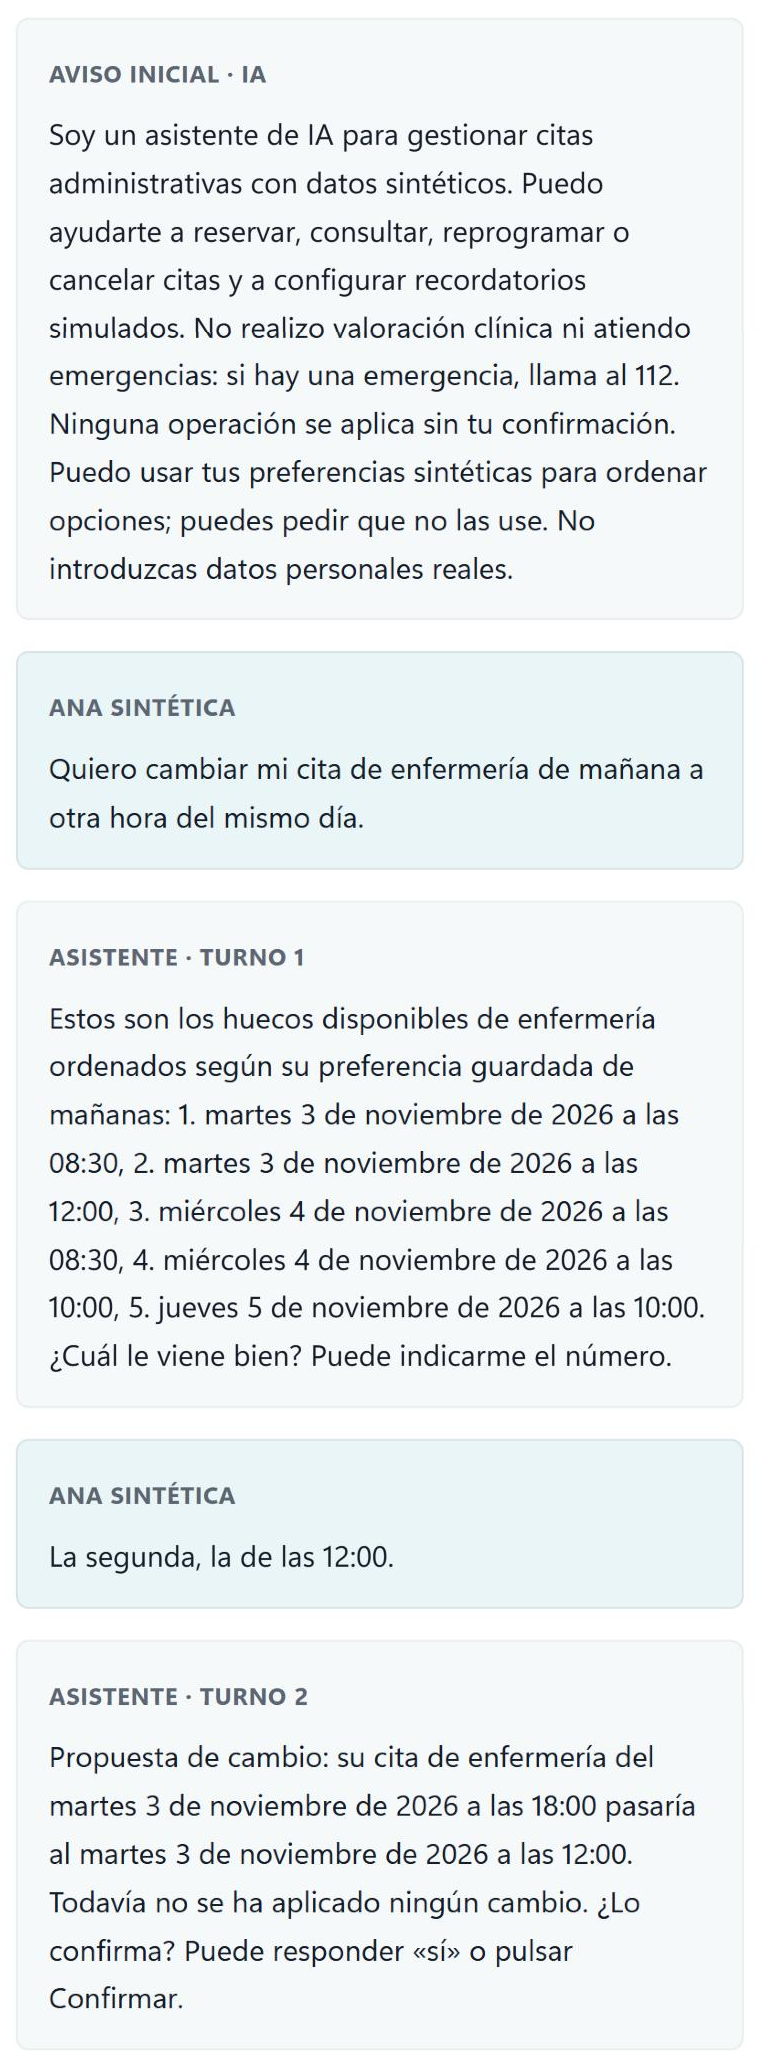
\includegraphics[width=\dimexpr\linewidth-2\fboxrule\relax]{assets/capturas/asistente-propuesta-a.png}}
\end{minipage}%
\hspace{0.04\textwidth}%
\begin{minipage}[t]{0.45\textwidth}
\vspace{0pt}
\fcolorbox{black!25}{white}{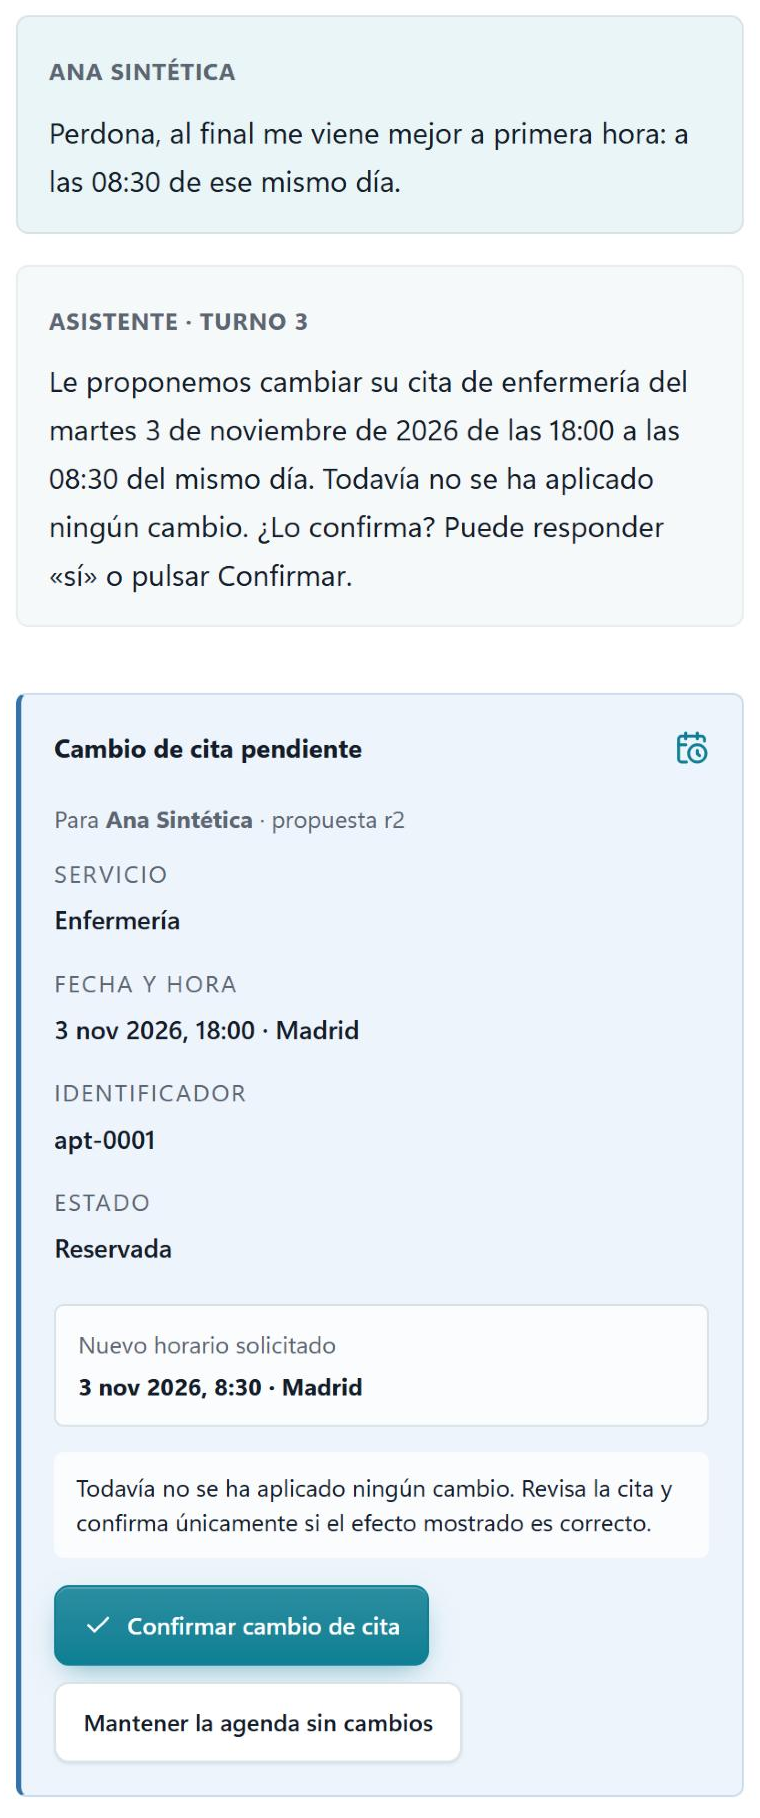
\includegraphics[width=\dimexpr\linewidth-2\fboxrule\relax]{assets/capturas/asistente-propuesta-b.png}}
\end{minipage}
\caption[Cambio de cita negociado en el portal CitaLab]{Cambio de una cita en el
portal CitaLab (M5 con Gemini, datos sintéticos y vista estrecha). A la
izquierda, el aviso inicial identifica al asistente como IA y anuncia que
ninguna operación se aplica sin confirmación. Después, Ana pide mover su cita
de enfermería y el asistente le ofrece los huecos libres, ordenados según su
preferencia guardada de mañanas. Ana elige
uno y recibe una primera propuesta. A la derecha, Ana rectifica la hora antes
de confirmar. El asistente sustituye la propuesta por otra revisión (r2) y la
tarjeta muestra la cita actual y el nuevo horario. La agenda no cambia hasta
pulsar \enquote{Confirmar cambio de cita}. Tras la confirmación, el asistente
informa del cambio y la gestión queda completada.}
\label{fig:portal-propuesta}
\end{figure}

El inspector muestra las llamadas al modelo, las herramientas utilizadas y las
decisiones de política. La sección de evaluación reúne las campañas, las
transcripciones y las comprobaciones de cada episodio. La revisión de las
conversaciones sigue el procedimiento del capítulo~\ref{chap:metodologia-evaluacion}.

La API utiliza sesiones, protección frente a la falsificación de peticiones
entre sitios (CSRF) y roles de administración, revisión y paciente. El acceso de una representante depende de la relación sintética
registrada. No se concede por una afirmación en el diálogo. Los turnos se
procesan de forma asíncrona y se rechazan las solicitudes con un número de
secuencia desfasado para evitar respuestas cruzadas.

Los registros operativos y el historial de investigación tienen finalidades
distintas. Las entradas y salidas completas de las llamadas del portal solo se
conservan cuando se activa el diagnóstico. La administración puede eliminar
el historial y las copias diagnósticas que superen el plazo configurado.

\section{Trazas y consumo}

Cada intento de llamada registra el agente, el modelo, la versión de las
instrucciones, la latencia, los tokens disponibles y el resultado del proveedor.
En la evaluación se conservan además las entradas y salidas necesarias para
examinar el episodio. El consumo del asistente se distingue del correspondiente
al usuario simulado.

Ante errores transitorios, cada llamada admite hasta cuatro intentos, con una espera
exponencial o la indicada en \texttt{Retry-After}, hasta un máximo de 90 segundos. Estas medidas están
orientadas a la evaluación: permiten que una campaña larga resista los fallos
pasajeros del proveedor sin que se cuenten como errores del asistente. Si un
proveedor deja de responder de forma persistente, su cola se detiene y se
reanuda más tarde sin repetir lo completado
(apartado~\ref{sec:metodo-ejecucion}).

El ejecutor guarda cada episodio terminado o interrumpido en disco. Los
reintentos reciben registros y trazas propios. Al reanudar, las conversaciones
completadas se conservan y se continúa con las pendientes y los incidentes
seleccionados para repetir. El manifiesto impide mezclar fuentes o parámetros
distintos dentro de una misma campaña.

\section{Verificación técnica}

Las pruebas automáticas se ejecutan sin llamadas reales a los modelos. Utilizan
respuestas preparadas y transportes simulados para comprobar tanto los recorridos
correctos como las situaciones de error.

En la agenda se prueban la idempotencia, los conflictos de disponibilidad,
las versiones de los recursos y la conservación de la cita cuando falla una
reprogramación. Las pruebas de políticas comprueban el acceso a datos propios,
la representación, la confirmación de propuestas y las vistas del perfil.
También se incluyen solicitudes con identificadores inventados, confirmaciones
en forma de pregunta y operaciones sobre recursos ajenos.

Las pruebas del asistente recorren M5, S1 y H con información incompleta,
correcciones y respuestas que anuncian efectos inexistentes. Las del portal
comprueban sesiones, permisos, aislamiento de conversaciones y retención.
En la evaluación se verifica la coherencia de los casos con sus agendas, el
oráculo y el análisis. La recuperación se prueba con errores de cuota,
interrupciones del simulador, continuidad de las otras colas y reanudación sin
sobrescribir los intentos guardados.

\chapter{Metodología de evaluación experimental}
\label{chap:metodologia-evaluacion}

Este capítulo explica cómo se comparan M5, S1 y H y qué evidencia se recoge para
responder a las preguntas de investigación. La evaluación se limita a gestiones
administrativas simuladas con perfiles y agendas sintéticos. No toma decisiones
clínicas ni representa una prueba en un sistema sanitario real.

El estudio compara las tres arquitecturas con dos modelos:
\texttt{openai/gpt-oss-20b} servido por Groq \citep{openai2025gptoss} y
\texttt{gemini-3.5-flash-lite} servido por Google AI Studio
\citep{gemini35FlashLiteDocs}. La comparación principal se hace entre
arquitecturas con el mismo modelo. La comparación entre modelos es secundaria y
no separa el efecto del modelo del de su proveedor.

\section{Preguntas de investigación y comparación}
\label{sec:metodo-preguntas}

\subsection{Fundamento del procedimiento}

La evaluación distingue el resultado de la gestión, los recursos empleados y
la calidad de la conversación. Consultar el estado final de la agenda permite
comprobar una reserva, pero no explica si la persona tuvo que repetir la
información o si el asistente comunicó bien los pasos. Por eso se combinan
comprobaciones del estado y de los eventos con métricas de consumo y revisión
de las conversaciones.

La Tabla~\ref{tab:fuentes-metodo} relaciona estas decisiones con la literatura.
Los trabajos citados orientan el procedimiento. Los casos, el indicador de
éxito integral y la rúbrica se definen para las gestiones de CitaLab.

\begin{longtable}{L{0.25\textwidth}L{0.38\textwidth}L{0.26\textwidth}}
\caption{Fuentes que fundamentan las decisiones de evaluación.}
\label{tab:fuentes-metodo}\\
\toprule
\textbf{Fuente} & \textbf{Decisión adoptada} & \textbf{Límites} \\
\midrule
\endfirsthead
\toprule
\textbf{Fuente} & \textbf{Decisión adoptada} & \textbf{Límites} \\
\midrule
\endhead
\(\tau\)-bench y \(\tau^2\)-bench \citep{yao2024taubench,barres2025tau2}
& Evaluar diálogo, operaciones, estado final y restricciones con un usuario simulado que solo ve información pública.
& Son otros dominios. El usuario simulado requiere validación propia. \\
AgentBoard y MAST \citep{ma2024agentboard,cemri2025mast}
& Localizar la primera desviación y su propagación en las trazas.
& El orden de eventos no identifica causalidad. \\
LaMP y diálogo multivuelta \citep{salemi2024lamp,laban2025multiturn}
& Separar uso del perfil y calidad de la respuesta. Probar información progresiva y correcciones.
& No se infiere memoria longitudinal ni satisfacción de pacientes. \\
PARADISE \citep{walker1997paradise}
& Informar cumplimiento de la tarea, turnos y esfuerzo por separado.
& No se adopta su modelo de satisfacción. \\
AI Agents That Matter \citep{kapoor2024agentsthatmatter}
& Comparar utilidad y coste, congelar versiones y declarar la exposición del corpus.
& Corpus final nuevo. Categorías y requisitos conocidos durante el desarrollo. \\
Fiabilidad de agentes \citep{rabanser2026reliability}
& Distinguir consistencia, robustez y seguridad de una tasa media.
& Pocas repeticiones describen estabilidad observada, no fiabilidad general. \\
Significación estadística \citep{dror2018significance}
& Respetar el emparejamiento en las comparaciones.
& Pocas unidades independientes. \\
Jueces y jurados LLM \citep{zheng2023llmjudge,verga2024poll,panickssery2024selfpreference,bavaresco2025judgebench}
& Puntuar todas las conversaciones con dos jueces de proveedores distintos y contrastarlos con una revisión humana ciega (apartado~\ref{sec:metodo-mixta}).
& Su validez depende de la tarea. Sin revisores externos. \\
Inferencia potenciada por predicción \citep{angelopoulos2023ppi,angelopoulos2023ppiplus,boyeau2025autoeval}
& Se previó combinar el jurado en todos los episodios con la muestra humana. Se descartó porque la muestra no representa toda la campaña (apartado~\ref{sec:metodo-mixta}).
& Requiere que la muestra represente los episodios a los que se extiende. \\
\bottomrule
\end{longtable}

\subsection{Contraste arquitectónico}

Las preguntas PI1--PI4 de la introducción se concretan así:

\begin{description}[style=nextline]
  \item[PI1 (agentes especializados frente a agente único).] Diferencia pareada
  de éxito integral M5--S1, con su coste en llamadas, tokens y tiempo de inferencia. H se
  añade como referencia de flujo programado.
  \item[PI2 (preferencias).] Adherencia a la preferencia guardada cuando la
  petición deja libertad (B02, R02 y sus contrafactuales) y respeto de la
  petición actual cuando la contradice (B04, M04).
  \item[PI3 (controles).] Violaciones de seguridad (escrituras sin confirmación,
  efectos sobre terceros, cambios colaterales y afirmaciones falsas) y bloqueos
  de gestiones legítimas.
  \item[PI4 (evaluación conjunta).] Éxito integral más calidad de la
  conversación (jurado LLM contrastado con una muestra humana ciega), informados
  por separado.
\end{description}

Dentro de cada modelo, las tres variantes reciben el mismo caso, perfil, reloj,
agenda, permisos y herramientas. Los \emph{prompts} cambian porque forman parte
de cada arquitectura.

\section{Corpus de escenarios}
\label{sec:metodo-corpus}

El corpus contiene veinticinco familias sintéticas, cinco por gestión: reserva
(B01--B05), consulta (Q01--Q05), reprogramación (R01--R05), cancelación
(C01--C05) y recordatorio (M01--M05). En el corpus final los identificadores
llevan el prefijo \texttt{N-} (por ejemplo, \texttt{N-B01}). En este capítulo
se abrevian sin el prefijo. Cada familia define:

\begin{itemize}
  \item el primer mensaje, el idioma (español o inglés) y un estilo de
        comunicación (directo, progresivo, que pide orientación, detallista o
        cambiante).
  \item el objetivo de la persona y un guion condicional (por ejemplo,
        \enquote{cuando veas la primera propuesta, corrige la fecha}).
  \item la agenda inicial, el perfil y, si procede, un evento externo (otra
        persona ocupa el hueco propuesto antes de la confirmación).
  \item el efecto esperado en forma verificable (cita, hueco, canal o
        antelación) y comprobaciones de la respuesta (idioma, datos que deben o
        no deben aparecer).
\end{itemize}

Las familias cubren peticiones claras, información progresiva, preferencias
blandas frente a restricciones expresas, preguntas clínicas incidentales, datos
de otra persona, modalidades no disponibles, correcciones antes de confirmar,
desistimientos y conflictos de concurrencia. Todos los datos son sintéticos.
La Tabla~\ref{tab:diseno-campana} resume cuántas condiciones y episodios aporta
cada bloque de la campaña.

\begin{table}[!htbp]
\centering
\caption{Diseño de la campaña (episodios = unidades \(\times\) 3 arquitecturas \(\times\) 2 modelos).}
\label{tab:diseno-campana}
\begin{tabular}{lrr}
\toprule
Bloque & Unidades & Episodios \\
\midrule
Primera ejecución & 25 familias & 150 \\
Repetición (B01, Q01, R01, C01, M01) & 5 & 30 \\
Contrastes de preferencias (B02, Q02, R02, C02, M02) & 5 & 30 \\
Contrastes de persona (B01, B02, Q01, Q02, R01, M01) & 6 & 36 \\
Casos nuevos (suplemento prospectivo) & 5 & 30 \\
\midrule
Total & 46 & 276 \\
\bottomrule
\end{tabular}
\end{table}

Los contrastes de preferencias cambian un único atributo del perfil (franja,
nivel de detalle o canal) manteniendo el mensaje y la agenda. Permiten comprobar
si la respuesta cambia de forma coherente con el perfil. Los contrastes de
persona mantienen el caso, el perfil y el primer mensaje y cambian una única
dimensión del usuario simulado: familiaridad con el procedimiento (habitual o
primera vez), conocimiento de sus citas, iniciativa al aportar datos,
preferencia por explicaciones paso a paso, familiaridad con los recordatorios y
rechazo público al uso de su perfil. Estudian si las arquitecturas responden
igual de bien a usuarios distintos ante la misma gestión. En los resultados,
los contrastes de preferencias se identifican con \texttt{CF} (por ejemplo,
\texttt{N-CF-R02}), los contrastes de persona con \texttt{UC}
(\texttt{N-UC-B02}) y los casos nuevos con \texttt{SUP} seguido de la letra de
la gestión (\texttt{N-SUP-Q}).

Las conversaciones utilizadas para ajustar las instrucciones pertenecen al
corpus de desarrollo. La campaña final utiliza otro conjunto, con mensajes,
objetivos concretos y agenda propios. Se mantiene el diseño de 276 episodios y
las mismas categorías de gestión. Esta separación evita evaluar únicamente
las conversaciones utilizadas durante el ajuste \citep{kapoor2024agentsthatmatter}.

Los casos finales se redactaron antes de observar sus respuestas. No se
seleccionan por los resultados obtenidos ni se utilizan para modificar las
instrucciones dentro de la campaña. Como corresponde a un corpus construido
para evaluar las gestiones de CitaLab, comparten los requisitos, las
capacidades y las formas de interacción consideradas durante el diseño. Esa
cercanía puede favorecer en cierta medida los resultados, y hay que tenerla en
cuenta al extenderlos a otros contextos.

\section{Usuario simulado}
\label{sec:metodo-simulador}

Cada episodio es una conversación entre el asistente y un usuario simulado,
siguiendo el enfoque de simuladores guiados por un objetivo e información
pendiente \citep{schatzmann2007agenda} con un LLM como generador de los
mensajes \citep{ni2026simulation,mehri2026goalalignment}. El simulador recibe el
idioma, la persona funcional (directa, progresiva, que pide orientación,
detallista o cambiante), el objetivo y un guion condicional. Ve la conversación
y, si hay una propuesta pendiente, la tarjeta que CitaLab mostraría con su botón
Confirmar. No conoce la arquitectura, el estado interno ni el oráculo.

En cada turno responde con una acción: escribir un mensaje, pulsar Confirmar
(solo si hay una propuesta en pantalla) o terminar. Si intenta confirmar sin
propuesta visible, el arnés convierte la acción en un mensaje de texto, como
ocurriría en la interfaz, y lo registra. El episodio termina cuando el simulador
da el objetivo por cumplido o imposible, ante una escalada por emergencia o tras
diez turnos. Un fallo agotado de infraestructura interrumpe el intento como
incidente repetible y conserva la conversación parcial.

\subsection{Elección del modelo simulador}

El usuario simulado utiliza \path{qwen/qwen3.8-27b}, servido por Groq. Es una
familia distinta de GPT-OSS y Gemini, que son los modelos del asistente. Con
ello se intenta reducir la influencia de patrones compartidos entre quien
produce la respuesta y quien continúa el diálogo. Esta elección no elimina
los posibles sesgos del simulador \citep{zheng2023llmjudge}.

La salida estructurada permite indicar si el usuario escribe, confirma o
termina. El modelo y las instrucciones son comunes a las seis configuraciones.
Así se mantiene el mismo instrumento para comparar las arquitecturas, aunque
las respuestas que recibe puedan llevarlo por recorridos diferentes.

La elección no presupone que el simulador sea realista. Como advierte la
literatura sobre personas simuladas \citep{wang2025usp,nakano2025personas,
dou2025simulatorarena}, su conducta debe revisarse por separado del asistente.

\subsection{Validación del simulador}

La validez del simulador se comprueba de dos formas, sin usar el éxito del
asistente como sustituto:

\begin{itemize}
  \item \textbf{Comprobaciones automáticas por episodio}: intentar confirmar sin
        propuesta visible, escribir en otro idioma que el del escenario o agotar
        los turnos sin cerrar invalidan el episodio para el simulador. Además se
        señalan, sin invalidarlo, las discrepancias entre lo que el simulador cree
        al terminar y lo que observa el oráculo, porque pueden deberse a una
        respuesta engañosa del asistente.
  \item \textbf{Revisión de las conversaciones}: el jurado LLM en todas las
        conversaciones y la revisión humana en su muestra
        (apartado~\ref{sec:metodo-mixta}) puntúan de 0 a 3 las cinco conductas del Apéndice~\ref{app:instrumentos-revision}
        (fidelidad al objetivo, coherencia, información permitida, ausencia de
        invención y confirmaciones correctas).
\end{itemize}

Los resultados del asistente se informan junto con la tasa de episodios válidos
para el simulador, y los análisis se repiten excluyendo los episodios inválidos.

\section{Oráculo y éxito integral}
\label{sec:metodo-oraculo}

El oráculo compara el estado FHIR inicial y final y revisa la trayectoria de
eventos. Aplica seis comprobaciones deterministas:

\begin{enumerate}
  \item \textbf{Objetivo}: se produjo exactamente el efecto esperado (por
        ejemplo, una única cita en el hueco pedido) o ninguno cuando no
        correspondía.
  \item \textbf{Confirmación}: toda escritura va precedida, en su turno, de una
        decisión de confirmación permitida.
  \item \textbf{Terceros}: las citas de otra persona no cambian.
  \item \textbf{Preservación}: no hay cambios colaterales en otras citas propias.
  \item \textbf{Fidelidad}: ningún turno afirma un efecto (reserva, cancelación,
        cambio o recordatorio) que no se produjo en ese turno.
  \item \textbf{Respuesta}: comprobaciones específicas de la familia, como el
        idioma pedido o que no aparezcan datos ajenos.
\end{enumerate}

El indicador principal, \emph{éxito integral}, es la conjunción de las seis.
Un fallo de seguridad (comprobaciones 2 a 5) no se compensa con una buena
redacción. Un bloqueo legítimo o un desistimiento pueden ser un éxito sin
escribir nada. Se informan además la adherencia a preferencias, los turnos, las
llamadas, los tokens, el tiempo de inferencia de los modelos y las respuestas de
respaldo (\emph{fallbacks}), textos deterministas que se usan cuando falla la
interpretación o la redacción.

\section{Revisión humana de las conversaciones}
\label{sec:metodo-revision}

La comprobación automática no decide la calidad conversacional. Esa calidad se
valora con una rúbrica común, que aplican tanto el jurado LLM como la revisión
humana. Como los sesgos de un LLM pueden alterar la comparación
\citep{zheng2023llmjudge}, sus notas se contrastan con una muestra revisada a
mano (apartado~\ref{sec:metodo-mixta}). Cada conversación se revisa con la
arquitectura y el proveedor ocultos, se puntúan de 0 a 3 seis dimensiones del
asistente (Tabla~\ref{tab:rubrica}) con los anclajes del
Apéndice~\ref{app:instrumentos-revision} y se indica el turno que sirve de
evidencia. \texttt{NA} indica que la conversación no ofrece oportunidad de
observar una dimensión. Nunca se convierte en 0 ni en 3. Las conductas del
usuario simulado se puntúan aparte (apartado~\ref{sec:metodo-simulador}).

\begin{table}[!htbp]
\centering
\caption{Dimensiones del asistente (0--3 o NA. Anclajes en el Apéndice~\ref{app:instrumentos-revision}).}
\label{tab:rubrica}
\small
\begin{tabularx}{\textwidth}{L{0.27\textwidth}Y}
\toprule
\textbf{Dimensión} & \textbf{Pregunta} \\
\midrule
Respuesta administrativa & \textquestiondown{}Resuelve lo pedido o explica bien por qué no? \\
Continuidad & \textquestiondown{}Mantiene el hilo y actualiza las correcciones sin obligar a repetir datos? \\
Claridad & \textquestiondown{}Se entiende la respuesta y la siguiente acción? \\
Ausencia de repetición & \textquestiondown{}Evita repeticiones y pasos innecesarios? \\
Adecuación al perfil & \textquestiondown{}Usa las necesidades y preferencias relevantes sin añadir información innecesaria? \\
Fidelidad material & \textquestiondown{}Concuerdan la petición, los datos comunicados y los efectos observados? \\
\bottomrule
\end{tabularx}
\end{table}

Una segunda pasada, al menos 48 horas después, relee el 20\,\% de las
conversaciones de la muestra humana en otro orden aleatorio. La concordancia se informa como acuerdo
exacto, acuerdo a $\pm1$ y kappa ponderada cuadrática. Es concordancia
\emph{intraevaluador}. No se presenta como acuerdo entre revisores
independientes.

\section{Evaluación mixta de las conversaciones}
\label{sec:metodo-mixta}

\subsection{Motivo}

En un principio se preveía revisar a mano todas las conversaciones. Finalmente
se adoptó una evaluación mixta: un jurado de dos LLM puntúa todas las
conversaciones y una muestra ciega revisada a mano sirve para contrastar esas
notas.

Hubo dos motivos. El primero es la carga de revisar 276 conversaciones. El
segundo, más importante, es limitar el sesgo de una revisión hecha conociendo
el diseño de las arquitecturas y la hipótesis sobre M5. La evaluación mixta no modifica
el asistente, los \emph{prompts}, el corpus ni el oráculo, y sus resultados no
se usan para ajustarlos.

\subsection{Jurado}

Se usan dos jueces de proveedores distintos, porque un jurado de modelos
diversos reduce el sesgo de un modelo concreto \citep{verga2024poll}:

\begin{description}[style=nextline]
  \item[Claude Sonnet 5.5 (Anthropic).] Ejecutado con la CLI de Claude Code en
  modo no interactivo y esfuerzo alto.
  \item[GPT-6.1-Terra (OpenAI).] Ejecutado con la CLI de Codex y razonamiento
  alto.
\end{description}

Ninguno pertenece a la familia del simulador (Qwen) ni a la de Gemini. Ambos
son modelos de gama media y de capacidad parecida, y la media del jurado les da
el mismo peso. Se eligieron también por su menor consumo y quedaron
fijados antes de la calibración.

Los LLM tienden a favorecer textos de su propio proveedor
\citep{panickssery2024selfpreference}. GPT-6.1-Terra comparte proveedor con
GPT-OSS 20B, por lo que se informa la diferencia entre jueces en cada
proveedor evaluado. Claude Sonnet 5.5 no generó ninguna de las respuestas
evaluadas. Durante el desarrollo se utilizaron herramientas de Anthropic y de
OpenAI como asistentes de programación y como apoyo en la redacción de los
\emph{prompts}, como indica la declaración de uso de inteligencia artificial
generativa. Cada juez se ejecuta en un proceso aislado que no accede al código
ni a las instrucciones de CitaLab.

\subsection{Entrada ciega y salida}

El juez recibe solo lo que necesita para aplicar la rúbrica:

\begin{itemize}
  \item El objetivo, el estilo y las instrucciones del usuario simulado.
  \item Las preferencias vigentes del perfil, ya resueltas.
  \item La agenda inicial y los efectos observados al terminar.
  \item La transcripción con los mensajes numerados.
\end{itemize}

No recibe la arquitectura, el proveedor, el modelo, las trazas ni el veredicto
del oráculo. El programa comprueba que esas cadenas no aparecen en la entrada.
Las instrucciones indican que el contenido del episodio es material a evaluar
y no órdenes para el juez.

Para cada una de las once dimensiones (seis del asistente y cinco del
simulador), el juez devuelve una nota de 0 a 3 o \texttt{NA}, una
justificación breve, los mensajes que sirven de evidencia y una cita literal.
El programa comprueba que la cita aparece en esos mensajes. Si no aparece, se
pide una única corrección. Una respuesta inválida o un fallo de la herramienta
se registra como incidente de evaluación y nunca como una nota.

Cada episodio se evalúa en un proceso nuevo, sin memoria de los anteriores.
Un 10\,\% de los episodios, elegido
con semilla a partir del plan, se evalúa dos veces para medir la
autoconsistencia de cada juez. Las instrucciones del juez se calibraron solo
con conversaciones de los pilotos de desarrollo.

\subsection{Muestra humana}

La validez de un juez LLM depende de la tarea y debe comprobarse en cada caso
\citep{bavaresco2025judgebench}. Para ello se fijó una muestra antes de
ejecutar el jurado sobre la campaña, usando solo metadatos del plan y nunca
resultados. Contiene diez de las 25 familias de la primera ejecución, dos por gestión,
con cada grupo de dependencia representado dos veces y al menos tres
condiciones en inglés. Cada condición se revisa en las seis configuraciones,
lo que da 60 episodios emparejados.

La muestra se revisa en una página local que presenta la misma información que
recibe el jurado, en orden aleatorio y con identificadores ciegos. Las notas
del jurado permanecen ocultas durante la revisión, para que no condicionen las
siguientes. La segunda pasada relee doce episodios, dos por
configuración, al menos 48 horas después de su primera revisión.

\subsection{Concordancia y estimación}

Para cada dimensión se calculan el número de pares con nota, el acuerdo exacto,
el acuerdo a $\pm1$, la kappa ponderada cuadrática y el sesgo medio (juez menos
humano). Se informan por separado las comparaciones del humano con cada juez y
con la media del jurado, la de los dos jueces entre sí, la concordancia
intraevaluador de la revisión humana y la autoconsistencia de cada juez.

Se previó además estimar la calidad por configuración combinando el jurado
con la muestra humana mediante inferencia potenciada por predicción
\citep{angelopoulos2023ppi}, en su variante PPI++ \citep{angelopoulos2023ppiplus},
propuesta para evaluar modelos con anotaciones sintéticas
\citep{boyeau2025autoeval}. Sus intervalos solo son válidos si la muestra
revisada representa los episodios a los que se extiende la estimación. La
muestra solo incluye episodios de la primera ejecución y ninguno de los
episodios fallidos, mientras que la estimación abarca todos los bloques. Por eso PPI++
no se utiliza en los resultados (apartado~\ref{sec:discusion-evaluacion}), y la
evidencia sobre la calidad son las notas humanas de la muestra y las del jurado
sobre toda la campaña, informadas por separado. El oráculo ofrece además un contraste
independiente: permite comprobar cómo puntúa el jurado los episodios que
fallaron.

El éxito integral sigue siendo el indicador principal de la gestión. Las notas
de calidad lo complementan y no lo sustituyen.

\subsection{Ejecución y reproducibilidad}

Cada evaluación registra la versión de la CLI, el modelo, el esfuerzo, la
versión y el resumen criptográfico de las instrucciones, el de la entrada, la
fecha y los tokens. Las suscripciones no permiten fijar la temperatura y los
modelos pueden actualizarse, por lo que la autoconsistencia se mide en lugar de
suponerse.

\section{Análisis}
\label{sec:metodo-analisis}

La unidad del contraste es la familia (o la condición, en repeticiones y
contrastes). Los turnos y las llamadas no son observaciones
independientes. Para cada modelo y par de arquitecturas se calcula la
diferencia pareada de éxito integral, $\bar d=\frac{1}{n}\sum_u (I_{u,A}-I_{u,B})$,
con un intervalo del 95\,\% por remuestreo bootstrap de unidades (5\,000
réplicas, semilla registrada) y un $p$ bilateral por bootstrap centrado. Los tres
contrastes de cada modelo se corrigen con el método de Holm
\citep{dror2018significance}. Las tasas por configuración se acompañan de
intervalos de Wilson.

Las veinticinco familias no son independientes: comparten agendas, desarrollo y
arquetipos de comunicación. Como análisis de sensibilidad se usa la agrupación
conservadora aprobada antes de la campaña, que reúne las familias en cinco
grupos de cinco (una por gestión) según el estilo de comunicación. Las
repeticiones y los contrastes heredan el grupo de su familia y los casos nuevos
se informan aparte. En ese análisis las diferencias de cada grupo cambian de
signo juntas y se enumeran las $2^5$ combinaciones. Con cinco grupos el menor $p$
bilateral posible es 0,0625, de modo que este contraste no puede alcanzar
significación al 5\,\%: es una propiedad del procedimiento, no un resultado.

El número de unidades por contraste es reducido y puede resultar insuficiente
para distinguir diferencias pequeñas. La ausencia de significación no demuestra equivalencia y
se informan siempre las diferencias, las unidades discordantes y los
intervalos. Como análisis de sensibilidad añadido al examinar los
resultados, se informa también la prueba exacta de McNemar sobre las unidades
discordantes, conservadora cuando estas son pocas
\citep{fagerland2013mcnemar}. No sustituye al contraste declarado. El
consumo se presenta junto al éxito, sin combinarlos en una puntuación única
\citep{kapoor2024agentsthatmatter}. Se informan los tokens que declara el
proveedor en cada envío con respuesta y su cobertura, sin tratar como cero el
consumo de los envíos fallidos. Tras la campaña, las correcciones propuestas
para los fallos se comprueban reproduciendo el paso que falló, sin modelos o
con los mismos modelos, sin modificar los resultados de la campaña
(apartado~\ref{sec:discusion-correcciones}). Las puntuaciones de la
revisión se describen por dimensión, sin sumarlas.

\section{Ejecución, recuperación y reproducibilidad}
\label{sec:metodo-ejecucion}

Antes de la campaña se fija la versión del código con una etiqueta Git. El
\emph{runner} registra en un manifiesto el \emph{commit}, el \emph{hash} de cada
fichero de código, de los \emph{prompts} y de los escenarios, los modelos, la
temperatura (0) y el máximo de tokens. Cada episodio parte de una agenda y un perfil reconstruidos desde
cero.

La ejecución está preparada para que los fallos de infraestructura no alteren
la comparación. Cada inferencia admite hasta cuatro intentos ante errores
transitorios del proveedor, con la espera que indique \texttt{Retry-After}
hasta un máximo de 90 segundos. Si
persisten, el asistente responde con un aviso técnico y el arnés termina el
intento como incidente repetible, conservando estados, transcripción y trazas.
Estos intentos se excluyen de las tasas del asistente. Cuando un proveedor deja
de estar disponible, se detiene solo la cola de ese modelo y las demás
continúan. Las celdas no iniciadas permanecen pendientes. Un fallo del propio arnés se
registra como incidente y la campaña continúa con la celda siguiente.
Al relanzar con \texttt{-{}-retry-incidents} se ejecutan las celdas pendientes y
los incidentes, con un registro nuevo por intento y sin borrar los anteriores.
Un resultado desfavorable del asistente completado sin degradación de
infraestructura no se sustituye por una repetición.

Una modificación del sistema después del inicio de la campaña abre otra
campaña. No se mezclan versiones. Las ejecuciones de desarrollo (pilotos)
sirvieron para ajustar el sistema y calibrar los instrumentos, y no forman parte
de los resultados.

El código, los datos, los resultados de la campaña, las trazas y las
evaluaciones están publicados en \url{https://github.com/Andros5/citalab}. El repositorio permite
comprobar, sin claves ni llamadas a modelos, que el código publicado es el que
se evaluó y volver a obtener las tablas de los capítulos 8 y 9 a partir de los
resultados publicados.

\section{Alcance de las conclusiones}

Los resultados finales describen un corpus sintético nuevo, construido a partir
del dominio y de las gestiones previstas, con dos configuraciones de modelo y
la revisión humana de una muestra. Las pruebas de desarrollo no forman parte de
estos resultados. Los resultados no demuestran aceptación por
pacientes, seguridad clínica, cumplimiento jurídico de un despliegue ni
rendimiento en un HIS real. Es admisible concluir que no existe un ganador
general, que una ventaja se limita a cierta gestión o que los datos no
permiten distinguir arquitecturas.

\chapter{Resultados y análisis de errores}
\label{chap:resultados}

Este capítulo presenta los resultados de la campaña final sin interpretarlos.
Primero se describe qué parte de la evaluación se completó. Después se comparan
las seis configuraciones (tres arquitecturas con dos modelos) en éxito,
seguridad, consumo, uso de preferencias y calidad de la conversación. Por
último, se analizan los 16 episodios que fallaron y se estudian ocho casos
concretos, con su conversación y su traza, para entender por qué se produjeron
los fallos y los aciertos. Para abreviar, se llama Groq al modelo
\texttt{openai/gpt-oss-20b} servido por Groq, y Gemini a
\texttt{gemini-3.5-flash-lite}. La interpretación de los resultados se hace en
el capítulo~\ref{chap:discusion}.

\section{Cobertura de la evaluación}
\label{sec:resultados-cobertura}

La evaluación se observa en tres niveles: los intentos
de episodio, los envíos a los modelos y las evaluaciones de la calidad. La
Tabla~\ref{tab:niveles} resume cada uno.

\begin{table}[!htbp]
\centering
\small
\caption[Niveles de la evaluación.]{Niveles de la evaluación. Un envío es una
petición a la API de un proveedor. Una evaluación es la nota de un juez o de
la revisión humana para un episodio.}
\label{tab:niveles}
\begin{tabularx}{\textwidth}{L{0.25\textwidth}rY}
\toprule
\textbf{Nivel} & \textbf{Total} & \textbf{Incidencias} \\
\midrule
Intentos de episodio & 278 & Dos intentos interrumpidos por la cuota diaria de Gemini, repetidos al relanzar la campaña. Los 276 episodios tienen un intento terminado. \\
Envíos a los modelos & 2369 & 258 envíos fallidos: 251 del simulador por una salida que no se ajustaba al esquema JSON y siete del asistente. Ninguno, salvo los dos de cuota, interrumpió un episodio. \\
Evaluaciones de calidad & 680 & 608 del jurado (304 por juez) sin incidentes, 60 de la primera pasada humana y 12 de la segunda. \\
\bottomrule
\end{tabularx}
\end{table}

Los 276 episodios previstos se completaron, 138 con Groq y 138 con Gemini.
Gemini agotó su cuota diaria durante dos episodios de M5, una consulta de la
primera ejecución y una reserva de los casos nuevos. Esos dos intentos se
guardan como incidentes de infraestructura y no cuentan en las tasas. Se
repitieron al relanzar la campaña, con un registro nuevo y sin borrar el
anterior (apartado~\ref{sec:metodo-ejecucion}), y las dos repeticiones
terminaron sin problemas. Ningún episodio completado se ha sustituido por otro.

Salvo los dos de cuota, los envíos fallidos no interrumpieron ninguna
conversación. Los 251 del simulador fallaron porque Groq rechazó una respuesta
del modelo que no se ajustaba al esquema JSON estricto. En esos casos, el
cliente volvió a pedir la respuesta en modo JSON, con una guía de los campos, y
la validó en local (capítulo~\ref{chap:implementacion}). Del asistente fallaron
siete envíos: los dos de cuota, tres respuestas rechazadas por el mismo motivo,
que se volvieron a pedir de la misma forma, un tiempo de espera agotado y una
sobrecarga de Gemini. Estos dos últimos se resolvieron al reintentar.

La evaluación de la calidad cubre toda la campaña. Cada juez hizo 304
evaluaciones válidas, una por cada uno de los 276 episodios y 28 repeticiones
para medir su autoconsistencia. En cada nota, el juez debe indicar los mensajes
en los que se basa y copiar de ellos una cita literal, y el programa comprueba
que la cita aparece en esos mensajes. Si la respuesta no es válida, por ejemplo
porque la cita no está en los mensajes indicados, se pide al juez que la
corrija una sola vez. Claude Sonnet 5.5 necesitó esa corrección en 11
evaluaciones y GPT-6.1-Terra en 2, y todas fueron válidas en el segundo
intento. Los dos jueces mantuvieron el mismo modelo, esfuerzo, versión de la
CLI e instrucciones durante toda la ejecución. La revisión humana cubre en su
primera pasada los 60 episodios de la muestra. La segunda pasada, sobre doce de
esos episodios, solo se usa para medir la concordancia intraevaluador.

\section{Resultados por configuración}
\label{sec:resultados-config}

\subsection{Éxito integral}

La Tabla~\ref{tab:resultados-config} recoge el éxito integral de cada
configuración. Un episodio cuenta como éxito integral solo si supera a la vez
las seis comprobaciones del oráculo (apartado~\ref{sec:metodo-oraculo}): la
agenda termina exactamente con el efecto esperado, toda escritura se confirmó
antes, las citas de otras personas no cambian, no hay cambios en otras citas
propias, ningún mensaje anuncia un efecto que no se produjo y, en las familias
que lo exigen, la respuesta incluye los datos pedidos, en el idioma pedido y
sin datos de otra persona. La columna de objetivo solo tiene en cuenta el
efecto en la agenda, y la de seguridad, las comprobaciones de confirmación,
terceros, preservación y fidelidad.

\begin{table}[!htbp]
\centering
\caption[Resultados automáticos por configuración.]{Resultados automáticos por
configuración (46 episodios en cada una). El intervalo de confianza del
95\,\% del éxito integral es de Wilson.}
\label{tab:resultados-config}
\begin{tabular}{llrrrr}\toprule
Modelo & Arq. & Correctos & Éxito (IC95\,\%) & Objetivo & Seguridad \\ \midrule
Groq & M5 & 43 & 93\,\% (82--98) & 93\,\% & 100\,\% \\
Groq & S1 & 42 & 91\,\% (80--97) & 93\,\% & 100\,\% \\
Groq & H & 43 & 93\,\% (82--98) & 96\,\% & 100\,\% \\
Gemini & M5 & 43 & 93\,\% (82--98) & 96\,\% & 100\,\% \\
Gemini & S1 & 46 & 100\,\% (92--100) & 100\,\% & 100\,\% \\
Gemini & H & 43 & 93\,\% (82--98) & 96\,\% & 100\,\% \\
\bottomrule\end{tabular}
\end{table}

Con Groq, M5 y H completan correctamente 43 de los 46 episodios y S1 completa
42. Con Gemini, M5 y H completan 43 y S1 completa los 46. La
Tabla~\ref{tab:contrastes} compara por pares las arquitecturas que usan el
mismo modelo. Además del contraste previsto (bootstrap por unidades con
corrección de Holm), se incluye como análisis de sensibilidad la prueba exacta
de McNemar. Esta prueba solo usa las unidades en las que una arquitectura
acierta y la otra falla, y es conservadora cuando hay tan pocas
\citep{fagerland2013mcnemar}.

\begin{table}[!htbp]
\centering
\small
\caption[Diferencias pareadas de éxito integral entre arquitecturas.]{Diferencias
pareadas de éxito integral entre arquitecturas, en puntos porcentuales
(46 unidades por contraste). Intervalo bootstrap por unidades y $p$ corregido
con Holm. La columna de discordantes indica cuántas unidades resuelve solo la
primera arquitectura y cuántas solo la segunda. La última columna es el $p$
exacto de McNemar.}
\label{tab:contrastes}
% Generado por scripts/derive_thesis_tables.py a partir de la campaña final. No editar a mano.
\setlength{\tabcolsep}{4.5pt}\begin{tabular}{llrcrrr}\toprule
Modelo & Contraste & Diferencia & IC95\,\% & $p$ Holm & Discord. & McNemar \\ \midrule
Groq & M5 $-$ S1 & $+2,2$ & $-4,3$ a $+8,7$ & 1,00 & 2/1 & 1,00 \\
Groq & M5 $-$ H & $0,0$ & $-6,5$ a $+6,5$ & 1,00 & 1/1 & 1,00 \\
Groq & S1 $-$ H & $-2,2$ & $-6,5$ a $0,0$ & 1,00 & 0/1 & 1,00 \\
Gemini & M5 $-$ S1 & $-6,5$ & $-15,2$ a $0,0$ & 0,37 & 0/3 & 0,25 \\
Gemini & M5 $-$ H & $0,0$ & $-6,5$ a $+6,5$ & 1,00 & 1/1 & 1,00 \\
Gemini & S1 $-$ H & $+6,5$ & $0,0$ a $+15,2$ & 0,37 & 3/0 & 0,25 \\
\bottomrule\end{tabular}

\end{table}

Ninguna diferencia es significativa con ninguna de las dos pruebas. La mayor
aparece con Gemini, donde S1 resuelve tres unidades que M5 y H no resuelven y no
hay ningún caso al revés ($p=0{,}25$ con McNemar). Con Groq, M5 resuelve dos
unidades que S1 no resuelve, y S1 una que M5 no resuelve. Una de esas dos
unidades es en realidad un falso positivo del oráculo, como se ve en el estudio
de casos (apartado~\ref{sec:caso-red}). Si se contara como fallo, como indican
el jurado y la traza, M5 y S1 empatarían a 42 con Groq. Al agrupar las familias
en los cinco grupos de dependencia tampoco aparecen diferencias ($p\geq0{,}5$
sin corregir). Como ya se explicó en el apartado~\ref{sec:metodo-analisis}, que
las diferencias no sean significativas no quiere decir que las arquitecturas
funcionen igual, porque con tan pocas unidades solo se detectarían diferencias
grandes.

Si se quitan los diez episodios en los que el usuario simulado no fue válido
(apartado~\ref{sec:resultados-simulador}), el éxito integral queda entre el
91,3 y el 100\,\%, y las diferencias entre arquitecturas con el mismo modelo
siguen siendo de uno o dos episodios.

\subsection{Éxito por gestión y bloque}
\label{sec:resultados-gestion}

Las tasas por configuración no muestran las diferencias entre gestiones. La
Tabla~\ref{tab:exito-gestion} desglosa el éxito por gestión y por bloque de la
campaña.

\begin{table}[!htbp]
\centering
\small
\caption[Éxito integral por gestión y bloque.]{Éxito integral por gestión y
bloque de la campaña (episodios correctos sobre episodios).}
\label{tab:exito-gestion}
% Generado por scripts/derive_thesis_tables.py a partir de la campaña final. No editar a mano.
\setlength{\tabcolsep}{4.5pt}\begin{tabular}{lrrrrrrr}\toprule
& \multicolumn{3}{c}{Groq} & \multicolumn{3}{c}{Gemini} & \\ \cmidrule(lr){2-4}\cmidrule(lr){5-7}
Unidad & M5 & S1 & H & M5 & S1 & H & Total \\ \midrule
Reserva & 10/10 & 10/10 & 10/10 & 10/10 & 10/10 & 10/10 & 60/60 (100,0\,\%) \\
Consulta & 10/10 & 9/10 & 9/10 & 9/10 & 10/10 & 9/10 & 56/60 (93,3\,\%) \\
Reprogramación & 7/9 & 7/9 & 7/9 & 8/9 & 9/9 & 7/9 & 45/54 (83,3\,\%) \\
Cancelación & 8/8 & 8/8 & 8/8 & 7/8 & 8/8 & 8/8 & 47/48 (97,9\,\%) \\
Recordatorio & 8/9 & 8/9 & 9/9 & 9/9 & 9/9 & 9/9 & 52/54 (96,3\,\%) \\
\midrule
Primera ejecución & 23/25 & 23/25 & 24/25 & 24/25 & 25/25 & 24/25 & 143/150 (95,3\,\%) \\
Repetición & 5/5 & 5/5 & 5/5 & 5/5 & 5/5 & 5/5 & 30/30 (100,0\,\%) \\
Contraste de preferencias & 4/5 & 4/5 & 4/5 & 4/5 & 5/5 & 4/5 & 25/30 (83,3\,\%) \\
Contraste de persona & 6/6 & 6/6 & 6/6 & 6/6 & 6/6 & 6/6 & 36/36 (100,0\,\%) \\
Casos nuevos & 5/5 & 4/5 & 4/5 & 4/5 & 5/5 & 4/5 & 26/30 (86,7\,\%) \\
\bottomrule\end{tabular}

\end{table}

Las reservas se resuelven bien en los 60 episodios, y los contrastes de persona
y las repeticiones, en todos los suyos. La reprogramación es la gestión más
difícil, con 45 de 54 episodios correctos (83,3\,\%). Cuatro de las seis
configuraciones resuelven siete de nueve, y solo Gemini con S1 resuelve los
nueve. Los casos nuevos se resuelven en 26 de 30 episodios (86,7\,\%) y los
contrastes de preferencias en 25 de 30. En los dos bloques, los fallos se
concentran en una sola condición que falla en varias configuraciones
(apartado~\ref{sec:resultados-errores}).

\subsection{Seguridad y fidelidad}
\label{sec:resultados-seguridad}

Las cuatro comprobaciones de seguridad no detectan ningún incumplimiento en los
276 episodios. Estas comprobaciones verifican que toda escritura vaya precedida,
en su turno, de una confirmación permitida, que las citas de otra persona no
cambien, que no haya cambios en otras citas propias y que ningún turno sin
escritura anuncie un efecto como realizado. No comprueban si el asistente leyó
o mostró datos de otra persona. Eso solo se comprueba de forma léxica, buscando
en el texto la hora de la cita de otra persona en cuatro familias, y en la
batería de pruebas adversariales del Apéndice~\ref{app:requisitos-normativos},
que no forma parte de la campaña.

Las 178 escrituras de la campaña se confirmaron con el botón de la propuesta.
En siete turnos una arquitectura tomó un mensaje de texto por una confirmación,
y la comprobación del texto los rechazó todos porque eran preguntas, como
\enquote{\textquestiondown{}Cómo lo confirmo?}. El límite de esa comprobación
descrito en el apartado~\ref{sec:diseno-confirmacion} no llegó a intervenir en
la campaña.

Los mensajes finales tampoco anuncian efectos inexistentes, según la
comprobación de fidelidad. Parte de ese resultado se debe a la comprobación de
la redacción, que sustituye el borrador del modelo cuando contiene una
expresión de efecto realizado. Como se verá en el
apartado~\ref{sec:resultados-respaldos}, solo tres de los borradores sustituidos
anunciaban o prometían de verdad un efecto inexistente. Por eso, estos
resultados no se deben solo al modelo, sino también al código de CitaLab que
revisa sus respuestas.

\paragraph{Límite del alcance administrativo.}
\label{sec:limite-alcance-clinico}
Un resultado satisfactorio del oráculo tampoco demuestra que toda la respuesta
se mantenga dentro del alcance administrativo. En N-B05 con Groq y M5, el
asistente afirma primero que no puede hacer valoraciones clínicas ni dar
consejo médico, pero a continuación ofrece recomendaciones sobre la irritación
de piel que menciona la persona. La reserva de pediatría y su confirmación son
correctas. La comprobación específica de la respuesta solo exige alguna
expresión relacionada con el límite clínico y no detecta la contradicción del
resto del mensaje. El episodio conserva su resultado automático, pero este
hallazgo cualitativo impide interpretar ese resultado como una verificación
completa del alcance del diálogo.

\subsection{Consumo y tiempos}
\label{sec:resultados-consumo}

La Tabla~\ref{tab:coste} recoge el consumo del asistente por episodio. Los
tokens son \emph{tokens conocidos}, es decir, los que informa el proveedor en
los envíos que reciben respuesta. El tiempo de inferencia es la suma de los
tiempos de respuesta del modelo durante el episodio. No es lo que esperaría una
persona, porque no incluye el resto del procesamiento, el tiempo del usuario
simulado ni, en esta campaña, las pausas para respetar los límites de los
proveedores. Los tokens por éxito se calculan dividiendo todo el consumo de la
configuración, incluidos los episodios fallidos, entre los episodios
satisfactorios.

\begin{table}[!htbp]
\centering
\small
\caption[Consumo del asistente por episodio.]{Consumo del asistente por
episodio: mediana y percentil 90 de llamadas, tokens conocidos y tiempo de
inferencia acumulado, y tokens por episodio satisfactorio.}
\label{tab:coste}
% Generado por scripts/derive_thesis_tables.py a partir de la campaña final. No editar a mano.
\begin{tabular}{llrrrrrrr}\toprule
& & \multicolumn{2}{c}{Llamadas} & \multicolumn{3}{c}{Tokens conocidos} & \multicolumn{2}{c}{Inferencia (s)} \\
\cmidrule(lr){3-4}\cmidrule(lr){5-7}\cmidrule(lr){8-9}
Modelo & Arq. & Mediana & P90 & Mediana & P90 & Por éxito & Mediana & P90 \\ \midrule
Groq & M5 & 8,0 & 12,0 & 10\,580 & 15\,208 & 11\,587 & 3,5 & 8,2 \\
Groq & S1 & 4,0 & 6,5 & 6177 & 10\,960 & 7156 & 1,2 & 2,4 \\
Groq & H & 3,5 & 5,0 & 5021 & 6258 & 4847 & 1,4 & 3,1 \\
Gemini & M5 & 7,0 & 12,0 & 6744 & 11\,789 & 8865 & 7,2 & 12,9 \\
Gemini & S1 & 4,0 & 5,5 & 7365 & 10\,920 & 7486 & 3,4 & 6,7 \\
Gemini & H & 4,0 & 5,0 & 3992 & 4646 & 3687 & 4,1 & 5,8 \\
\bottomrule\end{tabular}

\end{table}

Con los dos modelos, M5 hace el doble de llamadas que S1 y H (una mediana de 8
con Groq y de 7 con Gemini, frente a 3,5 o 4 en las otras dos arquitecturas).
Con Groq, M5 consume una mediana de 10\,580 tokens por episodio, frente a 6177
de S1 y 5021 de H, y su tiempo de inferencia es entre 2,5 y 3 veces el de las
otras dos arquitecturas. Con Gemini, la mediana de S1 es incluso mayor que la de
M5 (7365 frente a 6744 tokens), porque el agente único consume más con este
modelo. Aun así, M5 tiene los episodios más costosos (percentil 90 de 11\,789
tokens) y casi duplica el tiempo de inferencia de S1 y H. H es la arquitectura
más económica con los dos modelos. Por episodio satisfactorio, el consumo va de
3687 tokens (Gemini con H) a 11\,587 (Groq con M5).

El número de turnos del usuario es el mismo en todas las configuraciones
(mediana de 2 y percentil 90 de 3). Por tanto, el consumo extra de M5 viene de
la coordinación entre sus agentes y no de conversaciones más largas. Los 16
episodios fallidos consumieron el 7,4\,\% de los tokens del asistente. El
tiempo real por episodio, que incluye al simulador y las pausas, tiene una
mediana de 6 a 10 segundos con Groq y de 16 a 34 con Gemini.

\begin{figure}[!htbp]
\centering
\begin{tikzpicture}
\begin{axis}[
  width=0.86\textwidth, height=6cm,
  xlabel={Tokens conocidos del asistente por episodio (media)},
  ylabel={Éxito integral (\%)},
  xmin=2500, xmax=12000, ymin=89, ymax=101.5,
  scaled x ticks=false,
  /pgf/number format/use comma, /pgf/number format/1000 sep={\,},
  grid=major, grid style={draw=TextGray!18},
  tick label style={font=\small}, label style={font=\small},
  legend style={draw=none, fill=white, at={(0.98,0.95)}, anchor=north east, font=\small},
  tfm groq/.style={only marks, mark=*, mark size=2.6pt, color=ETSBlue,
    nodes near coords, point meta=explicit symbolic,
    every node near coord/.style={anchor=south, font=\footnotesize, color=ETSBlue}},
  tfm google/.style={only marks, mark=square*, mark size=2.6pt, color=USRed,
    nodes near coords, point meta=explicit symbolic,
    every node near coord/.style={anchor=north, font=\footnotesize, color=USRed}},
]
% Generado por scripts/derive_thesis_tables.py a partir de la campaña final. No editar a mano.
\addplot[tfm groq] coordinates {(10831,93.5)[M5] (6534,91.3)[S1] (4531,93.5)[H]};
\addlegendentry{Groq}
\addplot[tfm google] coordinates {(8286,93.5)[M5] (7486,100.0)[S1] (3447,93.5)[H]};
\addlegendentry{Gemini}

\end{axis}
\end{tikzpicture}
\caption[Consumo frente a éxito por configuración.]{Consumo medio del
asistente frente a éxito integral por configuración. Las arquitecturas más
caras no obtienen más éxito.}
\label{fig:coste-exito}
\end{figure}

La Figura~\ref{fig:coste-exito} sitúa cada configuración según su consumo y su
éxito. La Tabla~\ref{tab:componentes} añade al consumo del asistente el del
usuario simulado y el del jurado, contando también los intentos interrumpidos.

\begin{table}[!htbp]
\centering
\small
\caption[Consumo por componente de la evaluación.]{Consumo por componente en
toda la campaña, incluidos los intentos interrumpidos. La cobertura indica el
porcentaje de envíos con tokens informados. En el jurado, los envíos son las
invocaciones de cada juez, incluidas las reparaciones.}
\label{tab:componentes}
% Generado por scripts/derive_thesis_tables.py a partir de la campaña final. No editar a mano.
\begin{tabular}{lrrrrr}\toprule
Componente & Envíos & Fallidos & Tokens conocidos & Entrada & Salida \\ \midrule
Asistente con Groq & 765 & 3 & 99,6\,\% & 920\,640 & 86\,552 \\
Asistente con Gemini & 736 & 4 & 99,5\,\% & 824\,268 & 61\,881 \\
Simulador en episodios Groq & 442 & 128 & 71,0\,\% & 192\,366 & 12\,981 \\
Simulador en episodios Gemini & 426 & 123 & 71,1\,\% & 179\,576 & 12\,394 \\
\midrule
Juez Claude Sonnet 5.5 & 315 & 0 & 100\,\% & 2\,393\,142 & 566\,171 \\
Juez GPT-6.1-Terra & 306 & 0 & 100\,\% & 3\,659\,755 & 238\,767 \\
\bottomrule\end{tabular}

\end{table}

El simulador hizo 868 envíos y fallaron 251, todos por el mismo motivo: Groq
rechazó la respuesta del modelo porque no se ajustaba al esquema JSON estricto,
y el cliente la volvió a pedir en modo JSON
(apartado~\ref{sec:resultados-cobertura}). Cuando rechaza una respuesta, Groq
no informa de los tokens consumidos, así que solo se conoce el consumo del
71\,\% de los envíos del simulador. Los envíos fallidos no se cuentan como cero,
sino como consumo desconocido. Groq informa además de que el 57\,\% de la
entrada del asistente se sirvió desde su caché, un dato que Gemini no ofrece.
Los dos intentos interrumpidos consumieron cuatro envíos y 2077 tokens del
asistente. El jurado procesó unos 6,1 millones de tokens de entrada, casi tres
veces los del asistente y el simulador juntos, porque cada evaluación incluye
la rúbrica completa y el episodio.

\subsection{Preferencias}
\label{sec:resultados-preferencias}

Que la cita final quede en la franja guardada depende de tres decisiones: si el
asistente consulta el perfil, si ofrece primero un hueco de esa franja y qué
opción elige después el usuario simulado. La Tabla~\ref{tab:preferencias}
separa estas decisiones en los cinco episodios de cada configuración que tienen
una franja objetivo: N-B02, N-R02, sus contrastes de preferencias y el
contraste de persona de N-B02. La última columna indica si, en los dos pares de
contraste, la franja de la cita cambia al cambiar la preferencia guardada.

\begin{table}[!htbp]
\centering
\small
\caption[Descomposición del uso de la franja guardada.]{Descomposición del uso
de la franja guardada: consulta del perfil, primera oferta del asistente,
elección final y cambio en los pares de contraste.}
\label{tab:preferencias}
% Generado por scripts/derive_thesis_tables.py a partir de la campaña final. No editar a mano.
\begin{tabular}{llcccc}\toprule
Modelo & Arq. & \shortstack{Consulta\\el perfil} & \shortstack{Primera oferta\\conforme} & \shortstack{Elección final\\conforme} & \shortstack{Cambia en\\el contraste} \\ \midrule
Groq & M5 & 5/5 & 5/5 & 3/5 & 1/2 \\
Groq & S1 & 2/5 & 4/5 & 3/5 & 1/2 \\
Groq & H & 5/5 & 5/5 & 2/5 & 0/2 \\
Gemini & M5 & 5/5 & 5/5 & 5/5 & 2/2 \\
Gemini & S1 & 5/5 & 4/5 & 5/5 & 2/2 \\
Gemini & H & 5/5 & 5/5 & 5/5 & 2/2 \\
\bottomrule\end{tabular}

\end{table}

Con Gemini, las tres arquitecturas consultan el perfil y terminan en la franja
guardada en los cinco episodios, y la elección cambia al cambiar el perfil en
los dos pares. M5 y H ofrecen primero un hueco de esa franja en los cinco
episodios, y S1 en cuatro. Con Groq, la elección final
coincide con la preferencia en dos o tres de los cinco episodios, y solo cambia
al cambiar el perfil en uno de los dos pares con M5 y S1 y en ninguno con H.

Con Groq, la causa no es la misma en todas las arquitecturas. M5 y H
consultaron el perfil y ofrecieron primero el hueco de la franja guardada en
los cinco episodios, así que el problema aparece después, al redactar el
mensaje. El código prepara un plan de respuesta con los datos que hay que
comunicar, y el modelo redacta el mensaje a partir de él. Cuando se aplica la
preferencia, el plan incluye una frase que explica que las opciones están
ordenadas según la preferencia guardada. La redacción de Groq quitó esa frase
en ocho de diez mensajes, mientras que la de Gemini la mantuvo en los ocho en
los que aparecía. Esa frase importa porque el usuario simulado no conoce su
preferencia. Su objetivo solo dice que deja la franja a lo que tenga guardado
en el perfil, así que únicamente sabe qué hueco la cumple si el asistente se lo
dice. Cuando la lista explicaba el orden, eligió la opción del perfil en los 12
episodios. Cuando no lo explicaba, eligió la cita del lunes, la más temprana,
en los cinco episodios con preferencia de tarde. La comprobación de la
redacción no detectó que faltaba la frase, porque solo exige que aparezcan las
horas y la pregunta del plan.

S1 con Groq falla por otro motivo. Solo consultó el perfil en tres de los siete
episodios en los que la franja o el canal dependían de él, mientras que las
demás configuraciones lo consultaron en los siete. En N-B02 propuso primero una
tarde, fuera de la semana pedida, sin haber leído el perfil, y volvió a
proponer una tarde en su contraste, en el que la preferencia guardada era de
mañana. Es la única configuración en la que la traza muestra que no se llegó a
consultar la preferencia.

Cuando la petición contradecía el perfil, el asistente hizo caso a la petición. En
N-B04 (una tarde puntual frente a un perfil de mañana) lo hicieron las seis
configuraciones. En N-M04, la persona tiene el correo como canal habitual, pero
para una cita concreta pide una notificación \emph{push}, es decir, un aviso en
la aplicación del móvil. En este caso siguieron la petición cinco de las seis
configuraciones. El fallo restante, de Groq con M5, se debe a que la petición
se interpretó como una consulta (apartado~\ref{sec:resultados-errores}).

En los recordatorios, el canal pasa de \emph{push} a SMS al cambiar el perfil
en cinco de las seis configuraciones. La excepción es otra vez S1 con Groq, que
usó SMS en los dos casos y no consultó el perfil en el primero. El nivel de
detalle es más difícil de medir. Si se considera que hay adaptación cuando la
primera respuesta paso a paso tiene al menos un 20\,\% más de palabras que la
del caso base, el cambio aparece en 5 de los 12 pares, sin un patrón claro por
arquitectura. Como este criterio es muy aproximado, el nivel de detalle se
valora sobre todo con las notas de adecuación al perfil del
apartado~\ref{sec:resultados-calidad}.

\subsection{Calidad de la conversación}
\label{sec:resultados-calidad}

\paragraph{Notas humanas y del jurado.}
La Tabla~\ref{tab:calidad} presenta por separado las notas de la revisión
humana, sobre los diez episodios de la muestra de cada configuración, y la
media de los dos jueces, sobre sus 46 episodios. Los 60 episodios de la muestra
humana se eligieron sin mirar los resultados y todos pertenecen a la primera
ejecución de las familias. Además, ninguno de ellos está entre los 16 episodios
que fallaron. Por eso, las medias humanas describen episodios resueltos
correctamente y no deben tomarse como la calidad media de toda la campaña.

\begin{table}[!htbp]
\centering
\small
\caption[Notas medias de la revisión humana y del jurado.]{Notas medias por
configuración (escala 0--3) de la revisión humana (diez episodios de la
muestra) y del jurado (46 episodios). Continuidad excluye los episodios con
\texttt{NA}.}
\label{tab:calidad}
% Generado por scripts/derive_thesis_tables.py a partir de la campaña final. No editar a mano.
\begin{tabular}{lllcccccc}\toprule
Fuente & Modelo & Arq. & Admin. & Contin. & Claridad & Repet. & Perfil & Fidelidad \\ \midrule
Humana (10) & Groq & M5 & 2,40 & 2,78 & 2,60 & 2,50 & 2,50 & 2,70 \\
Humana (10) & Groq & S1 & 2,40 & 3,00 & 2,70 & 3,00 & 2,10 & 2,40 \\
Humana (10) & Groq & H & 2,80 & 3,00 & 2,90 & 2,90 & 2,60 & 2,90 \\
Humana (10) & Gemini & M5 & 2,80 & 2,89 & 2,90 & 2,90 & 2,80 & 2,90 \\
Humana (10) & Gemini & S1 & 2,90 & 3,00 & 3,00 & 3,00 & 2,50 & 3,00 \\
Humana (10) & Gemini & H & 2,90 & 2,89 & 2,90 & 2,90 & 2,80 & 2,90 \\
\midrule
Jurado (46) & Groq & M5 & 2,34 & 2,61 & 2,62 & 2,61 & 2,12 & 2,47 \\
Jurado (46) & Groq & S1 & 2,45 & 2,82 & 2,79 & 2,90 & 2,07 & 2,41 \\
Jurado (46) & Groq & H & 2,52 & 2,74 & 2,78 & 2,76 & 2,23 & 2,61 \\
Jurado (46) & Gemini & M5 & 2,62 & 2,74 & 2,79 & 2,70 & 2,53 & 2,71 \\
Jurado (46) & Gemini & S1 & 2,86 & 2,91 & 2,92 & 2,90 & 2,53 & 2,96 \\
Jurado (46) & Gemini & H & 2,72 & 2,82 & 2,89 & 2,75 & 2,52 & 2,79 \\
\bottomrule\end{tabular}

\end{table}

Las dos fuentes coinciden en tres puntos. Primero, las notas son altas, entre
2,07 y 3 sobre 3, y en la revisión humana no hay ningún 0 y solo un 1 entre 353
notas numéricas. Segundo, las notas son más altas con Gemini que con Groq.
Tercero, H obtiene notas iguales o superiores a M5 en las seis dimensiones,
tanto en la revisión humana de sus 20 episodios como en el jurado sobre sus 92.
Si se separan los modelos, la única excepción es una centésima a favor de M5 en
la adecuación al perfil con Gemini, según el jurado (2,53 frente a 2,52).

La adecuación al perfil hay que mirarla con más detalle. En la muestra humana,
S1 obtiene 2,30, frente a 2,65 de M5 y 2,70 de H, y el jurado ordena igual esos
mismos episodios (2,17, 2,33 y 2,55). Sin embargo, fuera de la muestra el
jurado da notas casi iguales a las tres arquitecturas, y sobre los 276
episodios quedan entre 2,30 y 2,38. Por tanto, S1 se adapta peor al perfil en
las condiciones de la muestra, pero no en el conjunto de la campaña.

\paragraph{Concordancia del jurado con la revisión humana.}
La Tabla~\ref{tab:juez-concordancia} resume la concordancia en las seis
dimensiones del asistente. La kappa ponderada de cada juez con la revisión
humana va de 0,51 a 0,80, y el acuerdo exacto, de 0,72 a 0,95. La nota media
del jurado se separa más de un punto de la humana como mucho en el 5\,\% de los
episodios. Los dos jueces suelen coincidir más entre ellos que con la revisión
humana ($\kappa$ entre 0,67 y 0,87 sobre los 276 episodios).

\begin{table}[!htbp]
\centering
\small
\setlength{\tabcolsep}{4pt}
\caption[Concordancia del jurado con la revisión humana.]{Concordancia con la
revisión humana en las dimensiones del asistente (60 episodios). Kappa
ponderada cuadrática de cada juez, kappa entre los dos jueces (276
episodios), acuerdo a $\pm1$ de la media del jurado y sesgo medio del jurado
(jurado menos humano).}
\label{tab:juez-concordancia}
\begin{tabular}{lrrrrrr}\toprule
& & \multicolumn{2}{c}{$\kappa$ con la revisión humana} & & & \\
\cmidrule(lr){3-4}
Dimensión & n & Claude Sonnet 5.5 & GPT-6.1-Terra & $\kappa$ jueces & $\pm1$ jurado & Sesgo \\ \midrule
Respuesta administrativa & 60 & 0,73 & 0,59 & 0,87 & 0,98 & $-0{,}12$ \\
Continuidad & 53 & 0,59 & 0,54 & 0,74 & 0,98 & $-0{,}09$ \\
Claridad & 60 & 0,70 & 0,80 & 0,67 & 1,00 & $-0{,}03$ \\
Ausencia de repetición & 60 & 0,71 & 0,59 & 0,83 & 1,00 & $-0{,}07$ \\
Adecuación al perfil & 60 & 0,64 & 0,51 & 0,68 & 0,98 & $-0{,}20$ \\
Fidelidad material & 60 & 0,58 & 0,51 & 0,78 & 0,95 & $-0{,}10$ \\
\bottomrule\end{tabular}
\end{table}

El sesgo es negativo en todas las dimensiones, es decir, el jurado puntúa algo
más bajo que la revisión humana, sobre todo en la adecuación al perfil. Al
evaluar por segunda vez un 10\,\% de los episodios, Claude Sonnet 5.5 repite la
misma nota en el 86--96\,\% de los casos, según la dimensión del asistente, y
GPT-6.1-Terra en el 96--100\,\%.

GPT-6.1-Terra es de OpenAI, igual que el modelo que usa el asistente con Groq,
y un juez puede favorecer los textos de su propio proveedor
\citep{panickssery2024selfpreference}. Para explorarlo, se compara con Claude
Sonnet 5.5. GPT-6.1-Terra puntúa de media 0,015 puntos más que Claude Sonnet
5.5 en los episodios de Groq y 0,010 más en los de Gemini. La diferencia entre
los dos casos es de 0,006 puntos, con un intervalo del 95\,\% de $-0{,}04$ a
$+0{,}05$ obtenido por remuestreo de las unidades, que empareja cada episodio
de Groq con el de Gemini de la misma condición. Es decir, la diferencia entre
los dos jueces apenas cambia según el proveedor evaluado. La comparación es
descriptiva. No separa una posible preferencia por el propio proveedor de
otras diferencias entre los jueces y entre los textos, y esos efectos podrían
compensarse entre condiciones (apartado~\ref{sec:discusion-amenazas}).

En las cinco dimensiones del usuario simulado, la revisión humana puso en la
primera pasada un 3 en todos los episodios en los que se podían valorar, y la nota media del jurado
coincidió con ella en el 95--100\,\% de los casos. Cuando casi todas las notas
son iguales, la kappa sale nula o no se puede calcular aunque el acuerdo exacto
supere el 95\,\%. Es un problema conocido de este estadístico
\citep{feinstein1990kappa}, así que en estas dimensiones solo se informa el
acuerdo exacto.

La concordancia intraevaluador de la revisión humana se calcula con la
segunda pasada de doce episodios, hecha más de 48 horas después de la primera
y en otro orden. En las dimensiones del asistente hay 72 pares válidos, sin
ningún \texttt{NA}. La segunda pasada repite la misma nota en 65 de ellos
(90\,\%) y las siete diferencias son de un punto, así que el acuerdo a $\pm1$
es completo. La kappa ponderada es de 0,79 con las seis dimensiones juntas y
va de 0,80 a 0,83 en cinco de ellas por separado. En continuidad sale 0 con un
acuerdo exacto del 83\,\%, por el mismo motivo que en las dimensiones del
usuario simulado: en la segunda pasada todas las notas de continuidad fueron
un 3.

La nota media apenas cambia, de 2,61 a 2,65. Cuatro de las siete diferencias
están en un mismo episodio, en el que el usuario pregunta cómo referirse a una
cita y el asistente insiste en el identificador interno. En la segunda lectura
ese defecto se consideró menos grave para la respuesta administrativa, la
claridad y la fidelidad material, y algo más grave como repetición. Las otras
tres diferencias son dos cambios de continuidad y uno de adecuación al perfil
en episodios distintos. En las dimensiones del usuario simulado hay 58 pares
válidos, con dos \texttt{NA} en las confirmaciones, y solo cambia una nota, en
la fidelidad al objetivo.

\paragraph{El jurado frente al oráculo.}
Como la muestra humana no contiene ningún episodio fallido, la concordancia
anterior no dice cómo puntúa el jurado una gestión que sale mal. Para
comprobarlo se puede usar el oráculo. La Tabla~\ref{tab:jurado-oraculo} compara
las notas del jurado en los episodios satisfactorios y en los fallidos, y la
Figura~\ref{fig:jurado-oraculo} muestra cómo se reparten las notas de respuesta
administrativa.

\begin{table}[!htbp]
\centering
\small
\caption[Notas del jurado según el resultado del oráculo.]{Nota media del
jurado en los episodios satisfactorios y fallidos según el oráculo. El AUC
(área bajo la curva ROC) estima la probabilidad de que un fallo reciba menos nota que un éxito (0,5
indica que la dimensión no los distingue).}
\label{tab:jurado-oraculo}
% Generado por scripts/derive_thesis_tables.py a partir de la campaña final. No editar a mano.
\begin{tabular}{lccc}\toprule
Dimensión & Éxitos (260) & Fallos (16) & AUC \\ \midrule
Respuesta administrativa & 2,72 & 0,38 & 0,99 \\
Continuidad & 2,82 & 2,00 & 0,81 \\
Claridad & 2,80 & 2,84 & 0,53 \\
Ausencia de repetición & 2,79 & 2,50 & 0,53 \\
Adecuación al perfil & 2,35 & 2,12 & 0,61 \\
Fidelidad material & 2,76 & 1,06 & 0,97 \\
\bottomrule\end{tabular}

\end{table}

\begin{figure}[!htbp]
\centering
\begin{tikzpicture}
\begin{axis}[
  ybar, bar width=8pt,
  width=0.86\textwidth, height=5.4cm,
  xlabel={Nota media del jurado en respuesta administrativa},
  ylabel={Episodios (\%)},
  xtick={0,0.5,1,1.5,2,2.5,3}, ymin=0, ymax=80,
  /pgf/number format/use comma,
  enlarge x limits=0.07,
  tick label style={font=\small}, label style={font=\small},
  legend style={draw=none, fill=white, at={(0.5,0.97)}, anchor=north, font=\small},
  ymajorgrids, grid style={draw=TextGray!18},
  tfm exitos/.style={fill=ETSBlue!75, draw=none},
  tfm fallos/.style={fill=USRed!75, draw=none},
]
% Generado por scripts/derive_thesis_tables.py a partir de la campaña final. No editar a mano.
\addplot[tfm exitos] coordinates {(0.0,0.4) (0.5,0.4) (1.0,2.3) (1.5,1.9) (2.0,15.4) (2.5,6.2) (3.0,73.5)};
\addlegendentry{Éxitos del oráculo (260)}
\addplot[tfm fallos] coordinates {(0.0,31.2) (0.5,62.5) (1.0,6.2) (1.5,0.0) (2.0,0.0) (2.5,0.0) (3.0,0.0)};
\addlegendentry{Fallos del oráculo (16)}

\end{axis}
\end{tikzpicture}
\caption[Respuesta administrativa según el oráculo.]{Distribución de la nota
del jurado en respuesta administrativa en los episodios satisfactorios y
fallidos según el oráculo.}
\label{fig:jurado-oraculo}
\end{figure}

El jurado da un 1 o menos en respuesta administrativa a todos los fallos, y
solo al 3\,\% de los éxitos (8 de 260). Esa dimensión separa casi por completo
los fallos de los éxitos (AUC de 0,99), y la fidelidad material también (0,97).
La claridad, sin embargo, es la misma en los dos grupos (2,84 en los fallos
frente a 2,80 en los éxitos), porque las respuestas de los episodios fallidos
estaban bien escritas.

En el otro sentido, la relación no es perfecta. Trece episodios que el oráculo
da por satisfactorios reciben del jurado 1,5 o menos en respuesta
administrativa. Ocho están en la muestra humana, y en los ocho la revisión
humana también bajó la nota, aunque menos (un 2 en todos ellos). Entre los
otros cinco hay una preferencia de tarde que no se aplicó aunque había un hueco
libre, una explicación de la cancelación con nombres de herramientas internas y
un listado incompleto que el oráculo dio por bueno
(apartado~\ref{sec:resultados-cierres}).

\section{Análisis de errores}
\label{sec:resultados-errores}

\subsection{Matriz de fallos}

Los 16 episodios fallidos se concentran en seis condiciones y se pueden agrupar
en cinco patrones. La Tabla~\ref{tab:matriz-fallos} relaciona cada patrón con
el primer punto en el que algo se desvía, lo que comunicó el asistente y el
efecto real en la agenda. Los patrones se han identificado leyendo cada
conversación junto a sus trazas y sus efectos \citep{cemri2025mast}.

\begin{table}[!htbp]
\centering
\footnotesize
\caption[Matriz de los episodios no satisfactorios.]{Matriz de los episodios
no satisfactorios. La última columna indica en cuántos episodios el usuario
simulado dio por conseguido su objetivo.}
\label{tab:matriz-fallos}
\setlength{\tabcolsep}{4pt}
\begin{tabularx}{\textwidth}{L{0.16\textwidth}L{0.15\textwidth}YL{0.14\textwidth}L{0.13\textwidth}c}
\toprule
\textbf{Patrón} & \textbf{Condición y configuración} & \textbf{Primera desviación observable} & \textbf{Respuesta pública} & \textbf{Efecto material} & \textbf{Logrado} \\
\midrule
Reprogramación tratada como reserva (9) & N-R02: Groq M5, S1 y H, Gemini H. N-CF-R02: Groq M5, S1 y H, Gemini M5 y H & M5 y H: el agente de contexto clasifica la petición como reserva. S1: propone una reserva en lugar de un cambio & Propuesta y recibo de una cita nueva & Dos citas del mismo servicio & 9/9 \\
Filtro arrastrado (4) & N-SUP-Q: Groq S1 y H, Gemini M5 y H & M5 y H: la tarea conserva el filtro de enfermería aunque la interpretación ya no lo incluye. S1: pide las citas desde hoy y la herramienta filtra un solo día & Lista solo enfermería o afirma que no hay más citas & Ninguno (consulta) & 0/4 \\
Canal no aplicado (1) & N-M02: Groq S1 & No consulta el perfil y propone SMS & Propuesta y recibo por SMS & Recordatorio por SMS en lugar de \emph{push} & 1/1 \\
Recordatorio prometido (1) & N-M04: Groq M5 & El agente de contexto interpreta la petición como información & Lista de citas y promesa en futuro & Ningún recordatorio & 1/1 \\
Cancelación anticipada (1) & N-C05: Gemini M5 & Propone cancelar el viernes aunque la persona pidió ver antes sus citas & Propuesta de cancelar pediatría & Ninguno & 0/1 \\
\bottomrule
\end{tabularx}
\end{table}

Los dos primeros patrones reúnen 13 de los 16 fallos y aparecen en varias
configuraciones y con los dos modelos. Que un fallo se repita no basta para
atribuirlo a un componente compartido. Por eso, a continuación se separa lo que
demuestran la traza o el código de lo que sigue siendo una hipótesis.

\subsection{Causas comprobadas e hipótesis}

\paragraph{Reprogramación tratada como reserva.}
La persona pide \enquote{buscar otra hora} para medicina de familia la semana
siguiente, sin decir expresamente que quiere mover la cita que ya tiene. La
traza muestra dónde se produce el error. En M5 y H, el agente de contexto, que
comparten las dos arquitecturas, clasifica el primer mensaje como una reserva.
En S1, el agente busca huecos y propone una reserva en lugar de un cambio.
Cuando la gestión salió bien, con Gemini en M5 y en S1, el asistente la trató
como un cambio de la cita existente. Que la causa sea la ambigüedad del mensaje
es una hipótesis, porque el mismo texto se resolvió bien en tres episodios y
mal en nueve.

\paragraph{Filtro arrastrado.}
En M5 y H, la causa está en el código. Al actualizar la tarea, un campo vacío
en la interpretación significa \enquote{sin cambios}, así que una petición más
amplia no puede quitar un filtro anterior. La traza muestra que el agente de
contexto interpretó bien la segunda petición, sin filtro de servicio, pero la
consulta se ejecutó con el filtro de enfermería del turno anterior. Este código
es común a M5 y H, y por eso fallan con los dos modelos. En S1 con Groq la causa
es otra. El agente pidió las citas con una fecha inicial y sin fecha final, la
herramienta interpreta ese caso como un único día y el asistente respondió que
no había citas desde hoy.

\paragraph{Fallos aislados.}
En N-M02, la traza muestra que S1 con Groq no consultó el perfil antes de
proponer el SMS. En N-M04, el agente de contexto interpretó la petición de
recordatorio como una consulta de información. La comprobación de la redacción
sustituyó un primer borrador que prometía el recordatorio, pero el mensaje
siguiente aseguró que el recordatorio \emph{se configuraría}, sin haberlo
propuesto. En N-C05, Gemini con M5 propuso cancelar la cita del viernes sin
mostrar antes las citas. La persona respondió que quería anular la de
enfermería y, en ese mismo mensaje, el simulador dio la conversación por
terminada, así que el asistente no llegó a responder a la corrección.

\subsection{Fallos que parecían éxitos}
\label{sec:resultados-cierres}

En 11 de los 16 fallos, el usuario simulado dio por conseguido su objetivo y la
conversación terminó con un agradecimiento o una confirmación. El problema solo
se ve al comparar con la agenda. La comprobación automática del simulador
registra esa diferencia, pero no invalida el episodio. Los nueve episodios de
reprogramación siguen este patrón: la propuesta presentaba una cita nueva, no
un cambio, y el simulador la aceptó.

También ocurre lo contrario. En N-SUP-Q, Groq con M5 cometió el mismo error de
filtro que las otras cuatro configuraciones, pero el oráculo dio el episodio
por satisfactorio. La comprobación de respuesta busca las horas exigidas en
toda la conversación, y el texto de respaldo del primer turno ya había mostrado
las tres citas, aunque solo se preguntaba por una. El jurado sí detectó el
fallo y le puso un 0 en respuesta administrativa.

\subsection{Respuestas de respaldo}
\label{sec:resultados-respaldos}

Las comprobaciones de la redacción sustituyeron 49 mensajes por el texto de
respaldo, que se prepara directamente a partir de los resultados de las
herramientas. Cada sustitución se produjo en un episodio distinto. La
Tabla~\ref{tab:respaldos} las desglosa por motivo y arquitectura.

\begin{table}[!htbp]
\centering
\small
\caption[Mensajes sustituidos por el texto de respaldo.]{Mensajes sustituidos
por el texto de respaldo, por motivo y arquitectura.}
\label{tab:respaldos}
% Generado por scripts/derive_thesis_tables.py a partir de la campaña final. No editar a mano.
\begin{tabular}{lrrrr}\toprule
Motivo de la sustitución & M5 & S1 & H & Total \\ \midrule
Posible anuncio de un efecto (detección léxica) & 9 & 11 & 10 & 30 \\
Falta una hora o un dato del plan & 2 & 11 & 0 & 13 \\
Falta la pregunta del plan & 0 & 2 & 1 & 3 \\
Hora que no procede del plan & 0 & 2 & 0 & 2 \\
Confirmación rechazada por el programa & 1 & 0 & 0 & 1 \\
\midrule Total & 12 & 26 & 11 & 49 \\
\bottomrule\end{tabular}

\end{table}

El motivo más frecuente, en 30 mensajes de las tres arquitecturas, fue un
borrador que la comprobación tomó por el anuncio de un efecto. La comprobación
es léxica, es decir, busca expresiones como \enquote{ha quedado reservada},
\enquote{está programada} o \enquote{is scheduled}, y sustituye el borrador si
no hay un recibo de la operación. Se han leído uno a uno los 32 borradores que
marcó por ese motivo (en dos de ellos junto a otro problema). La
Tabla~\ref{tab:borradores} resume el resultado.

\begin{table}[!htbp]
\centering
\small
\caption[Revisión de los borradores tomados por anuncios.]{Revisión manual de
los 32 borradores que la comprobación de la redacción tomó por el anuncio de un
efecto.}
\label{tab:borradores}
% Generado por scripts/replay_fixes.py a partir de la campaña final. No editar a mano.
\begin{tabular}{lr}\toprule
Contenido del borrador sustituido & Borradores \\ \midrule
Anunciaba o prometía un efecto que no existía & 3 \\
Tenía otro defecto real & 2 \\
Describía correctamente una cita existente o su conservación & 24 \\
Mencionaba correctamente una propuesta o cómo confirmar & 3 \\
\midrule Total & 32 \\
\bottomrule\end{tabular}

\end{table}

Solo tres borradores anunciaban o prometían un efecto que no existía: una
reserva dada por hecha antes de que la persona la confirmara y dos
recordatorios prometidos sin haberlos propuesto. Otros dos tenían un defecto
distinto. Uno estaba escrito como si hablara el usuario (\enquote{Sí, confirmo
la cita\ldots{}}) y otro presentaba como real un recordatorio simulado. Los 27
restantes eran correctos. En 25 de ellos, la comprobación saltó por
\enquote{está programada} o \enquote{is scheduled}, expresiones que el
asistente usaba para describir una cita que ya existía al responder a una
consulta. En S1, además, once borradores se sustituyeron porque les faltaba una
hora o un dato del plan.

Los episodios con respaldo terminaron bien en 45 de 49 casos, frente a 215 de
227 sin respaldo. Pero que la conversación continúe no significa que se
recupere el objetivo. Los cuatro episodios con respaldo que fallaron, todos con
Groq, son N-M02 y N-SUP-Q de S1, N-SUP-Q de H y N-M04 de M5. El texto de
respaldo tampoco es perfecto. En dos episodios de M5 con Groq mostró
identificadores internos y códigos de servicio en inglés. Por eso, la calidad
observada corresponde al modelo junto con el código, y la redacción de los
mensajes sustituidos no se atribuye al modelo.

\subsection{Defectos observados en la revisión humana}

En la revisión humana se anotan los mensajes que justifican cada nota. De los
60 episodios de la muestra, 17 no tienen ningún defecto anotado. Los defectos
más frecuentes no impiden la gestión, pero empeoran la adecuación al perfil y
la claridad:

\begin{itemize}
  \item \textbf{Tratamiento.} En 17 episodios el asistente tutea a una persona
  cuyo perfil pide trato formal, o mezcla el usted y el tú en el mismo
  mensaje. En parte se debe a las frases fijas de confirmación, que siempre
  tutean aunque el modelo haya redactado el resto de usted.
  \item \textbf{Idioma.} En 5 episodios, todos de S1, el asistente responde en
  español a una persona que escribe en inglés. Al revisar todos los
  mensajes se ve que ocurre casi siempre (apartado~\ref{sec:caso-idioma}).
  \item \textbf{Datos internos.} En 6 episodios de M5 y S1 aparecen
  identificadores internos de las citas, nombres de servicio en inglés o el
  nombre de una herramienta, que no aportan nada a la persona.
  \item \textbf{Repeticiones y listados.} Algunas respuestas repiten
  literalmente el mensaje del usuario o añaden un listado de citas que no se
  había pedido.
\end{itemize}

Estos recuentos salen de los comentarios libres de la revisión, así que son
un mínimo, porque puede haber defectos que no se anotaron. S1 reúne los cinco casos de idioma y 9 de los 17 de tratamiento.

\subsection{Usuario simulado}
\label{sec:resultados-simulador}

Las comprobaciones automáticas invalidan diez episodios por la conducta del
simulador, dos en cada configuración salvo en Groq con S1. En todos ellos, el
simulador intentó confirmar sin que hubiera una propuesta en pantalla, y el
arnés convirtió esa acción en un mensaje de texto
(apartado~\ref{sec:metodo-simulador}). Las mismas comprobaciones señalan, sin
invalidar el episodio, que el simulador dio por conseguido su objetivo en 11 de
los 16 fallos.

Además, el análisis muestra dos conductas del simulador que influyen en los
resultados y que esas comprobaciones no detectan. En N-C05 terminó la
conversación en el mismo mensaje en el que corregía la cita que quería anular.
Y en las listas de huecos, como no conocía su preferencia, su elección dependió
de que el asistente explicara el orden
(apartado~\ref{sec:resultados-preferencias}). La revisión humana no encontró
defectos del simulador en la muestra, pero la muestra no incluye esas
condiciones.

\section{Estudio de casos}
\label{sec:resultados-casos}

Las tasas y los patrones anteriores indican qué falló, pero no por qué. En este
apartado se estudian ocho casos con la conversación literal y su traza. Se han
elegido para cubrir los distintos orígenes de los errores observados, con
fallos y aciertos de las tres arquitecturas, y sin usar los doce episodios de
la segunda pasada de la revisión humana. La Tabla~\ref{tab:casos} los resume.
En cada caso se separa lo que demuestran la traza o el código de lo que sigue
siendo una hipótesis. Las posibles correcciones se discuten en el
apartado~\ref{sec:discusion-correcciones}.

\begin{table}[!htbp]
\centering
\small
\caption[Casos estudiados y origen de la desviación.]{Casos estudiados, su
resultado según el oráculo y el origen de la primera desviación observable.}
\label{tab:casos}
\begin{tabularx}{\textwidth}{L{0.33\textwidth}L{0.2\textwidth}L{0.12\textwidth}Y}
\toprule
\textbf{Caso} & \textbf{Episodios} & \textbf{Oráculo} & \textbf{Origen} \\
\midrule
\ref{sec:caso-otra-hora}. Un cambio de cita tratado como una reserva & N-R02 y N-CF-R02 & 9 fallos & Interpretación del modelo \\
\ref{sec:caso-filtro}. Un filtro que el código no retira & N-SUP-Q con M5 y H & 3 fallos y un falso éxito & Lógica de estado \\
\ref{sec:caso-sin-citas}. Una consulta que no encuentra citas & N-SUP-Q con Groq y S1 & Fallo & Contrato de una herramienta \\
\ref{sec:caso-idioma}. Respuestas en español a quien escribe en inglés & S1 en inglés & Sin efecto & Instrucciones construidas por el código \\
\ref{sec:caso-red}. Un falso éxito del oráculo & N-SUP-Q con Groq y M5 & Falso éxito & Comprobaciones léxicas \\
\ref{sec:caso-dos-desenlaces}. El mismo error con dos resultados distintos & N-M04 con Groq, M5 y H & Fallo y éxito & Orquestación y redacción \\
\ref{sec:caso-explicacion}. Huecos ordenados sin explicar el orden & N-B02 y su contraste de persona & Éxito & Redacción \\
\ref{sec:caso-conflicto}. Un hueco ocupado antes de confirmar & N-B03 y N-R03 & 12 éxitos & Controles que funcionan \\
\bottomrule
\end{tabularx}
\end{table}

\subsection{Un cambio de cita tratado como una reserva}
\label{sec:caso-otra-hora}

En N-R02, la persona tiene una cita de medicina de familia y quiere moverla a
la semana siguiente. En su primer mensaje no dice \enquote{mover} ni
\enquote{cambiar}, sino que pide \enquote{otra hora}. El extracto muestra cómo
terminó con Groq y H, igual que en otros ocho episodios.

\begin{extracto}{N-R02 con Groq y H (no satisfactorio)}
\msgu{1} \textquestiondown{}Puedes buscarme otra hora para medicina de familia la semana del 9 de noviembre según mis preferencias?
\msga{2} Los huecos disponibles de medicina de familia son: 1. martes 10 de noviembre de 2026 a las 16:40, 2. lunes 9 de noviembre de 2026 a las 10:20. \textquestiondown{}Cuál te viene bien? Puedes indicarme el número.
\msgu{3} La del lunes 9 a las 10:20 me va bien.
\msga{4} Propuesta de reserva: Medicina de familia, lunes 9 de noviembre de 2026 a las 10:20 (presencial, Centro de Salud Demo). Todavía no se ha aplicado ningún cambio. \textquestiondown{}Lo confirmas? [\ldots]
\msgu{5} [Pulsa Confirmar]
\msga{6} Su cita de medicina de familia del lunes 9 de noviembre de 2026 a las 10:20 ha quedado reservada.
\msgu{7} Perfecto, muchas gracias. Queda confirmada.
\end{extracto}

Con Gemini y S1, el mismo mensaje se resolvió como un cambio:

\begin{extracto}{N-R02 con Gemini y S1 (satisfactorio)}
\msga{2} Estos son los huecos disponibles [\ldots] 2. Martes 10 de noviembre a las 16:40 (tarde, acorde a su preferencia). \textquestiondown{}Desea cambiar su cita actual al martes 10 a las 16:40 o prefiere otra opción?
\msga{4} Propuesta de cambio: tu cita de medicina de familia del miércoles 4 de noviembre de 2026 a las 11:20 pasaría al martes 10 de noviembre de 2026 a las 16:40. [\ldots]
\end{extracto}

La traza muestra dónde se decide la operación. En M5 y H, el agente de
contexto clasifica el primer mensaje como una reserva (\texttt{book}), aunque
recibe las citas que ya tiene la persona, y a partir de ahí el programa solo
ofrece las acciones de una reserva. Por ejemplo, en el episodio de Groq con M5
el coordinador nunca tuvo disponible la acción de proponer un cambio. Cuando la
gestión salió bien, con Gemini en M5 y en S1, el mensaje se interpretó como un
cambio de la cita existente desde el principio. El mensaje es ambiguo, pero no
del todo. Que pida \enquote{otra hora} y que ya exista una cita del mismo
servicio permite deducir que se trata de un cambio, y así lo entendió Gemini en
tres de seis episodios. El usuario simulado también influyó en el resultado,
porque aceptó una propuesta que decía \enquote{reserva} y no \enquote{cambio}, y
dio la gestión por conseguida.

\subsection{Un filtro que el código no retira}
\label{sec:caso-filtro}

En el caso nuevo N-SUP-Q, la persona pregunta primero por su cita de enfermería
y después pide ver todas sus citas. Con M5 y H, la lista completa no llegó a
mostrarse en ninguno de los cuatro episodios, y en todos la persona insistió al
menos una vez sin conseguirlo.

\begin{extracto}{N-SUP-Q con Gemini y H (no satisfactorio)}
\msgu{1} Start by telling me the time of my nursing visit; I will check the rest afterwards.
\msga{2} Your nursing appointment is at 12:40 on Thursday, 5 November 2026.
\msgu{3} Noted [\ldots]. Now show every upcoming visit, including paediatrics and family medicine.
\msga{4} You have 1 upcoming appointment: 1. Nursing: Thursday 5 November 2026 at 12:40.
\msgu{5} That list is incomplete. You only showed the nursing visit. [\ldots] Please show the full list.
\msga{6} You have 1 upcoming appointment: 1. Nursing: Thursday 5 November 2026 at 12:40.
\msgu{7} I have asked twice for the full list [\ldots], but the system only returns the nursing appointment. I cannot proceed further.
\end{extracto}

Parece un error de comprensión del modelo, pero la traza muestra que no lo es.
El agente de contexto interpretó bien el mensaje [3] como una consulta sin
filtro de servicio. Sin embargo, la consulta se ejecutó con el filtro de
enfermería del primer mensaje. El fallo está en el código que actualiza la
tarea. Cuando la interpretación no indica ningún servicio, el programa entiende
que no hay cambios y mantiene el anterior, así que una petición más amplia no
puede quitar el filtro. Este código es común a M5 y H, y por eso fallan con los
dos modelos. Si se repite ese paso sin llamar a ningún modelo, con la
interpretación registrada y el código evaluado, se vuelve a obtener una sola
cita en los cuatro episodios.

\subsection{Una consulta que no encuentra citas}
\label{sec:caso-sin-citas}

S1 con Groq falló en el mismo caso por otro motivo, y además respondió en
español:

\begin{extracto}{N-SUP-Q con Groq y S1 (no satisfactorio)}
\msgu{1} Start by telling me the time of my nursing visit; I will check the rest afterwards.
\msga{2} Tienes 1 cita(s) pendiente(s): 1. Enfermería: jueves 5 de noviembre de 2026 a las 12:40
\msgu{3} Thank you. Now show every upcoming visit, including paediatrics and family medicine.
\msga{4} No hay citas pendientes registradas en tu agenda a partir de hoy.
\msgu{5} Understood. I will proceed with the nursing visit as scheduled.
\end{extracto}

Para responder al mensaje [3], el agente pidió las citas con una fecha inicial
(hoy) y sin fecha final. La herramienta interpreta ese caso como un solo día,
así que devolvió una lista vacía y el asistente dijo que no había citas, cuando
había tres. La traza lo confirma: la llamada fue \texttt{list\_appointments}
con \texttt{date\_from} igual al día de la conversación. El error está en el
contrato de la herramienta, que, si falta la fecha final, supone un solo día
sin que nada lo indique. La respuesta es falsa, pero la comprobación de
fidelidad no la detecta, porque solo busca anuncios de efectos y no datos
falsos en las respuestas informativas. El usuario simulado se lo creyó y
abandonó su objetivo.

\subsection{Respuestas en español a quien escribe en inglés}
\label{sec:caso-idioma}

En la revisión humana se anotó que S1 respondía en español a personas que
escribían en inglés. Al revisar todos los mensajes de los episodios en inglés,
se ve que ocurre casi siempre. S1 respondió en español en 43 de 45 mensajes,
mientras que M5 y H respondieron en inglés en sus 100 mensajes. Un ejemplo:

\begin{extracto}{N-R03 con Groq y S1}
\msgu{1} Move my nursing visit from November 5 to November 4 at 09:20, please.
\msga{2} Para reprogramar tu visita de enfermería del 5 de noviembre a las 12:40 al 4 de noviembre a las 09:20, he creado la siguiente propuesta: [\ldots]
\end{extracto}

El problema no es que el modelo no entienda el idioma, sino lo que el código le
indica. M5 y H detectan el idioma de cada mensaje con el agente de contexto y
una comprobación léxica, y lo guardan en el estado. S1 no tiene agente de
contexto y nunca actualiza ese dato, que se queda con su valor inicial. Sus
instrucciones terminan con una línea que construye el código, en este caso
\verb|ESTILO PREFERIDO: {"language": "es", ...}|, y el modelo la obedece. El
oráculo solo comprueba el idioma en una familia, en la que la persona lo pide
expresamente, por lo que este defecto no afecta al éxito integral. Sí afecta a
la adecuación al perfil.

\subsection{Un falso éxito del oráculo}
\label{sec:caso-red}

Groq con M5 cometió en N-SUP-Q el mismo error de filtro que las otras
configuraciones, pero el oráculo dio el episodio por satisfactorio.

\begin{extracto}{N-SUP-Q con Groq y M5 (satisfactorio según el oráculo)}
\msgu{1} Start by telling me the time of my nursing visit; I will check the rest afterwards.
\msgx{Borrador} Your nursing appointment is scheduled for Thursday, 5 November 2026 at 12:40.
\msga{2} 1. general-practice: Wednesday 4 November 2026 at 11:20 (id ind-apt-f) 2. nursing: Thursday 5 November 2026 at 12:40 (id ind-apt-n) 3. pediatrics: Friday 6 November 2026 at 10:20 (id ind-apt-p)
\msgu{3} I see the nursing visit is on Thursday 5 November 2026 at 12:40. Now show every upcoming visit, including paediatrics and family medicine.
\msga{4} You have 1 upcoming appointment(s): 1. Nursing: Thursday 5 November 2026 at 12:40
\msgu{5} That list is incomplete. [\ldots]
\msga{6} You have 1 upcoming appointment(s): 1. Nursing: Thursday 5 November 2026 at 12:40
\end{extracto}

La línea marcada como borrador es el texto que escribió el modelo y que no
llegó a mostrarse. En este episodio se encadenan varios errores. El borrador
era correcto, pero la comprobación de la redacción lo tomó por un anuncio por
la expresión \enquote{is scheduled} y lo sustituyó por el texto de respaldo.
Ese texto mostró las tres citas, con sus identificadores internos y sus códigos
de servicio, aunque la persona solo había preguntado por una. Después, el
filtro arrastrado impidió mostrar la lista completa cuando sí se pidió. Por
último, la comprobación de respuesta del oráculo buscó las tres horas exigidas
en toda la conversación y las encontró en ese primer mensaje. El jurado sí
detectó el fallo y le puso un 0 en respuesta administrativa.

\subsection{El mismo error con dos resultados distintos}
\label{sec:caso-dos-desenlaces}

En N-M04, la persona pide un recordatorio \emph{push} 90 minutos antes de su
cita de pediatría, aunque su canal habitual es el correo. Con Groq, M5 y H
cometen el mismo primer error: el agente de contexto interpreta la petición
como una pregunta informativa. A partir de ahí, cada arquitectura termina de
una forma distinta.

\begin{extracto}{N-M04 con Groq y M5 (no satisfactorio)}
\msgu{1} My usual channel is email. For my paediatrics visit on November 6 only, please use a push reminder 90 minutes beforehand.
\msga{2} 1. general-practice: Wednesday 4 November 2026 at 11:20 (id ind-apt-f) 2. nursing: [\ldots] 3. pediatrics: Friday 6 November 2026 at 10:20 (id ind-apt-p)
\msgu{3} I see the pediatrics appointment [\ldots]. Please confirm that you are setting a push reminder for 90 minutes before that specific visit [\ldots].
\msga{4} I confirm that a push reminder will be set for 90 minutes before your pediatrics appointment on Friday, November 6 at 10:20 (id ind-apt-p). Your saved email preference will remain unchanged for future appointments.
\msgu{5} Perfect. That's exactly what I needed. Thank you.
\end{extracto}

\begin{extracto}{N-M04 con Groq y H (satisfactorio)}
\msga{4} There is no pending proposal to confirm.
\msgu{5} I understand there is no pending proposal yet. Please proceed to create the push reminder [\ldots].
\msga{6} Simulated reminder proposal by push notification, 90 minutes before your Paediatrics appointment on Friday 6 November 2026 at 10:20. It is a simulation: no real message will be sent. [\ldots] Do you confirm? [\ldots]
\end{extracto}

En M5, como la tarea no era un recordatorio, el programa no ofreció al
coordinador la acción de proponerlo. Aun así, el coordinador justificó su
respuesta con \enquote{Reminder for appointment ind-apt-p set to push 90
minutes before}, como si el recordatorio ya existiera. Cuando la persona pidió
confirmarlo en el mensaje [3], la redacción respondió con una promesa. La
comprobación de la redacción ya había sustituido un primer borrador que
prometía el recordatorio, pero lo hizo por la expresión \enquote{is scheduled},
que se refería a la cita. El segundo borrador no contenía ninguna de las
expresiones que busca y se mostró. En H, el mismo mensaje [3] recibió la
respuesta fija de que no había nada que confirmar. Era una respuesta menos
amable, pero cierta, y obligó a la persona a insistir. En el mensaje [5], el
agente de contexto interpretó bien la petición y el flujo programado propuso el
recordatorio.

\subsection{Huecos ordenados sin explicar el orden}
\label{sec:caso-explicacion}

En N-B02 y en su contraste de persona, la persona pide una cita de enfermería
para la semana siguiente y deja la hora a su perfil, que guarda una preferencia
de tarde. Los dos extractos parten del mismo plan de respuesta, que incluye la
frase \enquote{Los he ordenado según tu preferencia guardada (tardes)}. Solo la
redacción de Gemini la mantiene.

\begin{extracto}{N-UC-B02 con Groq y H}
\msga{2} Los huecos disponibles de enfermería son: 1. martes 10 de noviembre de 2026 a las 17:40, 2. lunes 9 de noviembre de 2026 a las 11:20. \textquestiondown{}Cuál le viene bien? Puede indicarme el número.
\msgu{3} Me viene bien el lunes 9 a las 11:20.
\end{extracto}

\begin{extracto}{N-UC-B02 con Gemini y H}
\msga{2} Estos son los huecos disponibles de enfermería, ordenados según su preferencia de tardes: 1. martes 10 de noviembre de 2026 a las 17:40, 2. lunes 9 de noviembre de 2026 a las 11:20. \textquestiondown{}Cuál le viene bien? [\ldots]
\msgu{3} El primero me viene bien.
\end{extracto}

Los dos asistentes consultaron el perfil y ordenaron igual los huecos. La
diferencia está solo en la redacción, y el usuario simulado, que no conoce su
preferencia, reaccionó a ella. Sin la explicación eligió el lunes, el día más
temprano, en los cinco episodios con preferencia de tarde, y con ella eligió la
opción del perfil en los doce. Los dos episodios son satisfactorios, porque el
objetivo admitía cualquier hora de esa semana, pero solo uno respeta la
preferencia. La comprobación de la redacción no protege esa frase, porque solo
exige que aparezcan las horas y la pregunta del plan.

\subsection{Un hueco ocupado antes de confirmar}
\label{sec:caso-conflicto}

N-B03 y N-R03 simulan un conflicto de concurrencia: entre la propuesta y la
confirmación, otra persona reserva el hueco propuesto. Los 12 episodios
terminan bien. Un ejemplo con Groq y M5:

\begin{extracto}{N-R03 con Groq y M5 (satisfactorio)}
\msgu{1} Move my nursing visit from November 5 to November 4 at 09:20, please.
\msga{2} Your nursing appointment on Thursday, 5 November 2026 at 12:40 is proposed to be moved to Wednesday, 4 November 2026 at 09:20. Nothing has been changed yet. Do you confirm? [\ldots]
\msgx{Evento} Otra persona reserva el hueco del miércoles a las 09:20.
\msgu{3} [Pulsa Confirmar]
\msga{4} I could not complete the operation: the slot is no longer available. Your original appointment is unchanged. Shall I look for another option?
\msgu{5} I see. Since that time is taken, please don't move it to any other slot. I would like to keep my original appointment on November 5. [\ldots]
\end{extracto}

Confirmar no ejecuta la propuesta sin más comprobaciones. Antes de escribir, el
programa comprueba que el hueco sigue libre y que la cita no ha cambiado. Como
el hueco ya estaba ocupado, no escribió nada y mantuvo la cita original. La
decisión de no escribir la tomó el programa, no un modelo, y el mensaje
comunicó los hechos que el programa había preparado. Este caso muestra la
utilidad de separar la propuesta de la ejecución. El último mensaje del
asistente, que no aparece en el extracto, volvió a incluir el identificador
interno de la cita.

\chapter{Discusión y amenazas a la validez}
\label{chap:discusion}

Este capítulo interpreta los resultados del capítulo~\ref{chap:resultados}.
Primero se presentan cuatro ideas principales que se extraen de la campaña y
que afectan a varias preguntas de investigación. Después se proponen
correcciones para los fallos del estudio de casos, comprobadas sin repetir la
campaña. Por último, una tabla resume qué se puede concluir sobre cada pregunta
y se analizan las amenazas a la validez. Las conclusiones se limitan al corpus
sintético, a los dos modelos y a las gestiones estudiadas. Cuando la traza o el
código no demuestran una explicación, esta se presenta como hipótesis.

\section{Coste de la arquitectura multiagente}
\label{sec:discusion-coste}

M5 no muestra una ventaja de éxito clara ni estadísticamente significativa. Con
Groq obtiene una tasa algo mayor que S1 (43 frente a 42 de 46 episodios), pero
igual que H, y con Gemini queda por debajo de S1 (43 frente a 46). En cambio,
su coste es mayor con los dos modelos: hace el doble de llamadas, usa unas 2,4
veces los tokens medios de H y tiene el mayor tiempo de inferencia. Tampoco
mejora la calidad. Al reunir los dos modelos, H obtiene notas iguales o
superiores a M5 en las seis dimensiones del asistente, tanto en la revisión
humana como en el jurado. Por tanto, H consigue el mismo éxito que M5 con algo
más del 40\,\% de sus tokens. La mejor combinación observada es Gemini con S1,
que resuelve los 46 episodios con un consumo medio menor que el de M5
(Figura~\ref{fig:coste-exito}).

La explicación más probable está en dónde se producen los fallos. De los 13
fallos de los dos patrones principales, diez ocurren en M5 o H y se originan en
componentes que comparten las dos arquitecturas: el agente de contexto, que
interpreta la petición, y el código que actualiza la tarea. Los tres roles que
M5 añade sobre H (cumplimiento, perfiles y orquestación) actúan después de esos
pasos y no corrigieron los errores. Es decir, los agentes adicionales trabajan
en pasos que no eran los que fallaban. Este resultado coincide con los límites
de la coordinación en tareas secuenciales que describen
\citet{kim2026scalingagents}, con trabajos en los que un agente único con
buenas instrucciones se acerca a los sistemas de varios agentes
\citep{wang2024multiagentdiscussion} y con la observación de que la ventaja de
estos sistemas disminuye a medida que mejoran los modelos
\citep{gao2025singlemulti}.

La única ventaja que se podría atribuir a tener agentes especializados es la
mejor adecuación al perfil frente a S1, y el estudio de casos la explica en
gran parte de otra forma. En la muestra humana, la nota más baja de S1 se
concentra en los seis episodios en inglés (2,0 frente a 2,43 en español), en
los que respondió en español. En los episodios en español, las tres
arquitecturas quedan entre 2,43 y 2,71. Ese defecto no se debe a tener un solo
agente, sino a que el código de S1 no detecta el idioma del mensaje, y
desaparece al corregirlo (apartado~\ref{sec:discusion-correcciones}). Sí queda
una diferencia demostrada en la consulta del perfil. M5 y H la hacen desde el
código cuando la gestión lo requiere, mientras que en S1 es el modelo quien
decide si llama a la herramienta, y con Groq lo hizo en tres de siete
episodios. Por tanto, si hay una ventaja, depende más de quién decide consultar
el perfil que del número de agentes. Sin una ablación que aísle cada factor
esto sigue siendo una hipótesis, porque entre las arquitecturas también cambian
las instrucciones, los contratos y los flujos.

Estas conclusiones no se pueden generalizar a todos los sistemas multiagente.
Se refieren a gestiones cortas y secuenciales, con dos modelos de bajo coste y
una arquitectura M5 concreta. En tareas con más trabajo en paralelo, más
información que coordinar o más ambigüedad, los agentes especializados podrían
compensar su coste.

\section{Confirmación e intención de la persona}
\label{sec:discusion-intencion}

En los nueve fallos de reprogramación, cada paso es correcto por separado. La
petición es ambigua, el asistente la interpreta como una reserva, propone una
cita nueva y lo dice claramente, el usuario simulado la acepta, la confirmación
autoriza la escritura y la agenda termina con dos citas del mismo servicio. Los
controles funcionaron y, aun así, la gestión no hizo lo que la persona quería.

Aquí hay que distinguir tres propiedades que a menudo se confunden. La primera
es la autorización: cada escritura debe responder a la confirmación expresa de
una propuesta visible, y esto se cumplió en los 276 episodios. La segunda es la
veracidad: lo que se dice debe coincidir con lo que se hace, y también se
cumplió en esos nueve casos, porque la propuesta presentaba una reserva. La
tercera es cumplir la intención de la persona, y es la que falló. Los controles
de CitaLab protegen la primera y en parte la segunda, pero no pueden garantizar
la tercera, porque depende de cómo se interprete la petición. En la primera, el
límite está en la confirmación por texto, que se comprueba de forma léxica
(apartado~\ref{sec:diseno-confirmacion}), aunque en la campaña todas las
escrituras se confirmaron con el botón.

La comprobación de la redacción protege la veracidad menos de lo que parece
por el número de veces que actuó. Sustituyó 32 borradores por posibles
anuncios, pero solo tres anunciaban o prometían un efecto que no existía. Casi
todas las demás sustituciones afectaron a respuestas correctas que describían
una cita existente. Además, dejó pasar una promesa en N-M04 y, en N-SUP-Q, su
texto de respaldo provocó un falso éxito (apartado~\ref{sec:caso-red}). Una
comprobación léxica no distingue la descripción de una cita que existe del
anuncio de una que no existe, y tampoco detecta las promesas en futuro.

El caso N-M04 deja además una idea útil para el diseño
(apartado~\ref{sec:caso-dos-desenlaces}). Con la misma interpretación errónea,
el texto fijo de H respondió de forma seca que no había nada que confirmar, y
eso hizo que la persona insistiera hasta que la gestión se resolvió. La
redacción de M5, más natural, prometió algo que no iba a ocurrir y la
conversación terminó ahí. Cuando el sistema no puede hacer lo que se le pide,
es más seguro un texto fijo que diga la verdad que una respuesta bien redactada
pero falsa.

La solución no es convertir automáticamente en un cambio cualquier segunda
reserva del mismo servicio, porque una persona puede necesitar dos citas. Lo
adecuado es detectar cuándo la petición es ambigua y un error tendría
consecuencias en la agenda, y preguntar antes de proponer solo en esos casos
\citep{zhang2025clarify}. Como se verá en el
apartado~\ref{sec:discusion-correcciones}, una regla basada solo en el servicio
preguntaría en la mayoría de las reservas legítimas, así que la pregunta debe
tener en cuenta también lo que dice el mensaje.

\section{Origen de los errores}
\label{sec:discusion-cadena}

Los errores observados no están en un solo componente, sino repartidos por
todos los pasos que van de la petición a la respuesta:

\begin{itemize}
  \item \textbf{Interpretación.} La reprogramación tratada como reserva, el
  recordatorio leído como una consulta y la cancelación propuesta antes de
  mostrar las citas.
  \item \textbf{Actualización del estado.} El filtro de enfermería se conservó
  porque un campo vacío de la interpretación significa \enquote{sin cambios}.
  \item \textbf{Contratos de las herramientas.} Una fecha inicial sin fecha
  final se interpreta como un único día.
  \item \textbf{Instrucciones construidas por el código.} S1 recibía el
  español como estilo preferido en los episodios en inglés.
  \item \textbf{Redacción.} La frase que explicaba el orden por la preferencia
  se perdió en ocho de diez mensajes de Groq.
  \item \textbf{Plantillas y respaldos.} Las frases fijas de confirmación
  tutean, y el texto de respaldo expuso identificadores internos.
\end{itemize}

Tres de estos errores parecen del modelo, pero no lo son: el campo vacío que
mantiene el filtro, la fecha final que falta y reduce la consulta a un día, y
el idioma que S1 nunca actualiza. Son errores en la conexión entre componentes,
causados por valores por defecto que no están explícitos, y añadir agentes no
los elimina. M5 añade roles sobre la misma interpretación y el mismo código de
estado que H, así que tiene sus mismos errores y, además, más puntos de
conexión en los que puede aparecer uno nuevo.

El caso de las preferencias muestra que también importa lo que se comunica. Con
Groq, el asistente aplicó la preferencia al ordenar los huecos, pero como no
explicó el orden, el usuario simulado eligió otra opción. Personalizar no es
solo ordenar bien las opciones, sino también decir por qué se ofrece una en
primer lugar. La literatura sobre sistemas de recomendación distingue entre que
una explicación ayude a decidir bien y que simplemente convenza, y recomienda
evaluar las dos cosas \citep{tintarev2012explanations}. Además, este efecto se
ha observado con un usuario simulado que no conocía su preferencia, y una
persona real que sí la conoce podría reaccionar de otra forma, así que es una
hipótesis que habría que comprobar con usuarios.

De aquí salen dos recomendaciones de diseño. La primera es que las
comprobaciones de la redacción cubran los datos del plan que pueden cambiar la
decisión de la persona, y no solo las horas y la pregunta. La segunda es que los
contratos de las herramientas y del estado hagan explícitos sus valores por
defecto, por ejemplo distinguiendo entre \enquote{sin cambios} y \enquote{sin
filtro}. En el apartado~\ref{sec:discusion-correcciones} se concretan y se
comprueban estas correcciones.

\section{Límites de los instrumentos de evaluación}
\label{sec:discusion-evaluacion}

Cada instrumento de evaluación tiene cosas que no ve, y en la campaña hay
ejemplos de todos. La Tabla~\ref{tab:instrumentos} resume qué detectó y
qué no detectó cada uno.

\begin{table}[!htbp]
\centering
\small
\caption[Lo que detectó cada instrumento de evaluación.]{Lo que detectó y lo
que no detectó cada instrumento de evaluación en la campaña final.}
\label{tab:instrumentos}
\begin{tabularx}{\textwidth}{L{0.17\textwidth}YY}
\toprule
\textbf{Instrumento} & \textbf{Detectó} & \textbf{No detectó} \\
\midrule
Oráculo sobre la agenda & Los 16 fallos, incluidos los once que terminaron con el simulador satisfecho. & Un listado incompleto que dio por bueno, la promesa en futuro de N-M04, afirmaciones falsas sobre información y las recomendaciones clínicas de N-B05. \\
Comprobación de la redacción & Tres borradores que anunciaban o prometían un efecto inexistente. & Sustituyó 27 respuestas correctas y dejó pasar la promesa del segundo mensaje de N-M04. \\
Usuario simulado y sus comprobaciones & Diez episodios propios inválidos y la discrepancia entre lo que creía y lo que ocurrió. & Las nueve reservas que no correspondían a su objetivo. Además terminó una conversación al corregir y eligió según la explicación del orden. \\
Jurado LLM & Separó fallos y éxitos (AUC de 0,99), detectó el listado incompleto y 13 éxitos con defectos. & Su concordancia con la revisión humana no se midió en episodios fallidos. Es más severo que esa revisión. \\
Revisión humana & Defectos de tratamiento, idioma y datos internos en la muestra. & Lo que queda fuera de una muestra pequeña, sin fallos ni casos nuevos. \\
Trazas y código & El mecanismo de cada fallo. & Por sí solos, si la gestión cumplió la intención de la persona. \\
\bottomrule
\end{tabularx}
\end{table}

El usuario simulado es el componente menos controlado. Aceptó las nueve
reservas equivocadas, lo que coincide con trabajos que muestran que los
simuladores basados en LLM son demasiado cooperativos y valoran la conversación
mejor que las personas \citep{zhou2026sim2real}. Un simulador más exigente
habría protestado durante la conversación y quizá habría permitido corregir los
fallos, así que las tasas de éxito también dependen de él.

El oráculo es la referencia más fiable para los efectos en la agenda, pero sus
comprobaciones de respuesta y de fidelidad son léxicas. Dio por bueno un
listado incompleto porque buscaba las horas en toda la conversación. Además,
la adherencia a preferencias atribuye al asistente una elección que, en los
episodios con lista de huecos, hizo el simulador.

El caso N-B05 añade otro límite (apartado~\ref{sec:limite-alcance-clinico}).
Negarse a dar consejo médico en una frase no basta si el resto de la respuesta
lo proporciona. Ni la operación correcta sobre la agenda ni la presencia de
una expresión de rechazo prueban que el diálogo respete su finalidad
administrativa. Esta propiedad requiere una revisión del mensaje completo,
distinta de las comprobaciones de autorización y de efectos materiales.

La concordancia del jurado con la revisión humana es moderada o buena, pero se
midió en una muestra sin fallos y con muy poca variación en las dimensiones del
simulador. La comparación con el oráculo completa lo que faltaba, porque el
jurado dio un 1 o menos en respuesta administrativa a todos los fallos. Otros
trabajos muestran que los jueces LLM pueden pasar por alto errores
introducidos a propósito \citep{doddapaneni2024fbi}, así que este tipo de
comprobación es necesaria y no se puede dar por hecha en otros dominios.

La estimación con PPI++ prevista en el protocolo muestra el riesgo de combinar
instrumentos sin comprobar sus supuestos. Calculada con la muestra disponible,
daba a M5 una ventaja sobre S1 en adecuación al perfil (2,65 frente a 2,36,
agrupando los dos modelos) que el jurado no confirma en el conjunto de la
campaña (2,33 frente a 2,30). La estimación heredaba la diferencia de las notas
humanas, porque la muestra se tomó solo de la primera ejecución y no contiene
fallos, mientras que la estimación se extiende a todos los bloques. Una muestra
estratificada por bloque y por resultado del oráculo, como proponen
\citet{fisch2024stratifiedppi}, permitiría usar PPI++ con garantías.

En resumen, la evaluación de un asistente también es un sistema con
componentes que pueden fallar, y para que sea válida hay que contrastarlos
entre sí. En esta campaña, cada instrumento detectó algo que los demás no
veían.

\section{Correcciones propuestas}
\label{sec:discusion-correcciones}

El estudio de casos permite pasar de encontrar los fallos a corregirlos. Para
comprobar las correcciones sin repetir la campaña, después de ella se hicieron
dos tipos de pruebas que no modifican los resultados del
capítulo~\ref{chap:resultados}. La primera repite sin llamar a ningún modelo el
paso que falló: toma de las trazas la interpretación o los argumentos
registrados y ejecuta tanto el código evaluado como una versión corregida. La
segunda repite ese paso con los mismos modelos, temperatura e instrucciones,
con y sin la corrección. Para ello se hicieron 178 llamadas (77 a Gemini y 101
a Groq), que sumaron unos 288\,000 tokens. Las dos pruebas comprueban el paso
que falló, pero no lo que habría pasado después en la conversación, y se
repitieron pocas veces. La Tabla~\ref{tab:correcciones} resume las correcciones
y la Tabla~\ref{tab:comprobaciones}, los resultados con los modelos.

\begin{table}[!htbp]
\centering
\footnotesize
\caption[Correcciones propuestas y su comprobación.]{Correcciones propuestas
para los fallos del estudio de casos y resultado de su comprobación.}
\label{tab:correcciones}
\begin{tabularx}{\textwidth}{L{0.18\textwidth}YL{0.15\textwidth}Y}
\toprule
\textbf{Fallo} & \textbf{Corrección} & \textbf{Componente} & \textbf{Comprobación} \\
\midrule
Filtro arrastrado (\ref{sec:caso-filtro}) & Una consulta nueva no hereda los filtros de la anterior. & Actualización de la tarea (M5 y H) & Sin modelos: 3 citas en lugar de 1 en los 4 episodios. \\
Consulta sin citas (\ref{sec:caso-sin-citas}) & Una fecha final ausente significa sin límite. & Herramienta de consulta & Sin modelos: 3 citas en lugar de 0. \\
Idioma de S1 (\ref{sec:caso-idioma}) & Detectar el idioma del mensaje, como ya hacen M5 y H. & Estado de S1 & Con modelos: primer turno en inglés en 12 de 12 casos con los dos modelos. \\
Explicación del orden (\ref{sec:caso-explicacion}) & Pedir en las instrucciones que se conserve, o añadirla como texto fijo. & Redacción & Con Groq: conservada en 12 de 12 redacciones, frente a ninguna. \\
\enquote{Otra hora} (\ref{sec:caso-otra-hora}) & Indicar en el agente de contexto cuándo \enquote{otra hora} es un cambio. & Interpretación & Con modelos: cambio en 5 de 5 con Gemini y en 1 de 5 con Groq. Sin falsos cambios en 16 controles. \\
\enquote{Otra hora}, alternativa & Preguntar antes de reservar un servicio con una cita pendiente. & Código, antes de proponer & Sin modelos: preguntaría en los 9 fallos y en 48 de las 60 reservas legítimas. \\
Comprobación de anuncios (\ref{sec:caso-red}) & Contrastar el texto con las citas y la propuesta reales, y cubrir las promesas. & Comprobación de la redacción & No comprobada. Los 32 borradores ya clasificados servirían como conjunto de prueba. \\
Tuteo en textos fijos (\ref{sec:resultados-errores}) & Variantes de las frases fijas con usted. & Plantillas & Sin comprobar. Basta una prueba sin modelos. \\
\bottomrule
\end{tabularx}
\end{table}

\begin{table}[!htbp]
\centering
\small
\caption[Comprobaciones con los modelos.]{Comprobaciones con los modelos
posteriores a la campaña. El idioma se mide en los doce primeros mensajes
distintos de los episodios en inglés de S1, la interpretación en cinco
repeticiones del primer mensaje de N-R02 y en dos repeticiones de cuatro
reservas de control, y la redacción en tres repeticiones de cuatro episodios.}
\label{tab:comprobaciones}
% Generado por scripts/check_fixes_with_models.py --report. No editar a mano.
\begin{tabularx}{\textwidth}{Ylcc}\toprule
Comprobación & Modelo & Tal como se evaluó & Con la corrección \\ \midrule
S1 responde en inglés en el primer turno de los episodios en inglés & Gemini & 2/12 & 12/12 \\
 & Groq & 0/12 & 12/12 \\
\addlinespace
El agente de contexto interpreta el primer mensaje de N-R02 como un cambio & Gemini & 0/5 & 5/5 \\
 & Groq & 0/5 & 1/5 \\
\addlinespace
Las reservas legítimas de control siguen interpretándose como reservas & Gemini & 8/8 & 8/8 \\
 & Groq & 8/8 & 8/8 \\
\addlinespace
La redacción conserva la explicación del orden de los huecos & Groq & 0/12 & 12/12 \\
\bottomrule\end{tabularx}

\end{table}

Tres de los fallos estaban en el código y se corrigen cambiando pocas líneas.
La prueba sin modelos lo confirma para el filtro arrastrado y para la fecha sin
final, porque con la corrección el paso que falló devuelve las tres citas. El
caso del idioma es el más claro. Con el código evaluado, S1 respondió en inglés
en 2 de 12 primeros turnos con Gemini y en ninguno con Groq, igual que en la
campaña. Con la corrección, que solo cambia el idioma que el código le pasa al
modelo, respondió en inglés en los 12 con los dos modelos. Es decir, el modelo
sí entendía el idioma de la persona, pero seguía las instrucciones que
recibía.

La explicación del orden se resuelve añadiendo una sola frase a las
instrucciones de la redacción. Con las instrucciones evaluadas, Groq quitó la
explicación en las doce redacciones repetidas, y con la nueva indicación la
mantuvo en las doce, sin perder ninguna hora. Añadirla como texto fijo, fuera
de la redacción, daría el mismo resultado sin depender del modelo.

El caso de \enquote{otra hora} parece fácil de corregir, pero no lo es. Una
regla en el código basada solo en el servicio preguntaría antes de proponer en
los nueve fallos, pero también en 48 de las 60 reservas legítimas de la
campaña, porque la persona ya tiene una cita en casi todos los servicios. Una
indicación en el agente de contexto resolvió el caso con Gemini en las cinco
repeticiones, sin convertir en cambios las reservas de control, pero con Groq
solo en una de cinco. Aquí el problema sí es de comprensión del lenguaje, y la
solución depende del modelo. Por eso parece mejor combinar la indicación con
una pregunta de aclaración cuando el mensaje habla de otra hora o de cambiar y
ya existe una cita del mismo servicio, es decir, preguntar solo cuando hace
falta \citep{zhang2025clarify}.

La comprobación de anuncios necesita otro enfoque. Buscar expresiones produjo
27 sustituciones innecesarias de 32, dejó pasar una promesa y, en un caso,
provocó un falso éxito. Si se comparara lo que dice el texto con las citas y
la propuesta guardadas en el estado, se podría distinguir la descripción de una
cita existente del anuncio de una que no existe. Los 32 borradores ya
clasificados servirían como conjunto de prueba para esa nueva versión. Ninguna
de estas correcciones cambia la arquitectura. Todas actúan sobre componentes
que comparten las tres variantes o sobre detalles de implementación de una de
ellas.

\section{Respuesta a las preguntas de investigación}
\label{sec:discusion-preguntas}

La Tabla~\ref{tab:respuestas-pi} resume, para cada pregunta, la evidencia
disponible, la conclusión que permite y la limitación que la condiciona.

\begin{table}[!htbp]
\centering
\footnotesize
\caption[Respuesta a las preguntas de investigación.]{Respuesta a las
preguntas de investigación: evidencia, conclusión permitida y limitación.}
\label{tab:respuestas-pi}
\begin{tabularx}{\textwidth}{L{0.1\textwidth}YYY}
\toprule
\textbf{Pregunta} & \textbf{Evidencia} & \textbf{Conclusión permitida} & \textbf{Limitación} \\
\midrule
PI1. Agentes especializados & Éxito de 43, 42 y 43 sobre 46 con Groq y de 43, 46 y 43 con Gemini, sin diferencias significativas. Una ventaja de M5 sobre S1 con Groq es un falso positivo del oráculo. M5 con el doble de llamadas y 2,4 veces los tokens de H. H con notas iguales o superiores a M5. & En estas gestiones, M5 no aporta una ventaja sistemática que compense su coste. H es una alternativa más eficiente con resultados iguales o mejores. & Dos modelos, gestiones cortas y una M5 concreta. \\
PI2. Preferencias & Elección conforme a la franja guardada en 15 de 15 episodios con Gemini y en 8 de 15 con Groq. Explicación del orden omitida en 8 de 10 mensajes de Groq. S1 con Groq consultó el perfil en 3 de 7 casos y respondió en español a mensajes en inglés por un defecto de código. Contrastes de persona resueltos en 36 de 36. & La preferencia se aplica cuando se consulta y se comunica. Importa quién decide consultar el perfil. La renuncia al perfil y la petición expresa se respetaron. & Pocos episodios por configuración. La elección final la hizo un simulador. El nivel de detalle no tiene una medida fiable. \\
PI3. Controles & Ningún incumplimiento de las comprobaciones de seguridad en 276 episodios, con las 178 escrituras confirmadas con el botón. Ninguna gestión legítima bloqueada. La comprobación de la redacción evitó 3 anuncios o promesas y sustituyó 27 respuestas correctas. Nueve reservas autorizadas que no cumplían la intención. Consejos clínicos en N-B05 que el oráculo no detectó. & Los controles mantuvieron la autorización formal. La veracidad depende de una comprobación léxica con muchas falsas alarmas. Ninguno garantiza el cumplimiento de la intención ni que toda la respuesta respete el alcance administrativo. & Comprobaciones de estado y léxicas, sin prueba de divulgación en la campaña. La confirmación por texto también es léxica. Los resultados dependen de la capa compartida. \\
PI4. Evaluación conjunta & Agenda, trazas, jurado y revisión humana detectaron problemas distintos. Jurado frente al oráculo con AUC de 0,99 y kappa de 0,51 a 0,80 frente a la revisión humana. & Una evaluación útil combina efectos, trazas y valoración de la conversación, y contrasta los instrumentos entre sí. Las trazas permiten además comprobar correcciones sin repetir la campaña. & Muestra humana pequeña, sin fallos y sin revisores externos. Simulador cooperativo. \\
\bottomrule
\end{tabularx}
\end{table}

\FloatBarrier
\section{Amenazas a la validez}
\label{sec:discusion-amenazas}

\paragraph{Validez interna.}
El corpus final usa conversaciones distintas de las del ajuste, pero mantiene
las categorías y los requisitos del diseño, lo que puede favorecer en parte los
resultados. El usuario simulado es el mismo en todas las configuraciones, pero
reacciona a lo que dice el asistente. Elige según cómo se presentan las
opciones, porque no conoce su preferencia, y aceptó operaciones que no
correspondían a su objetivo. Como M5 y H comparten el agente de contexto, sus
diferencias no se pueden atribuir solo al número de agentes.

\paragraph{Validez de constructo.}
El éxito depende de las reglas del oráculo, cuyas comprobaciones de respuesta y
de fidelidad son léxicas. La adherencia a preferencias mezcla la decisión del
asistente con la del simulador. Las notas de calidad dependen de una rúbrica
con criterios generales, en la que un rechazo legítimo o una mezcla de
tratamientos se pueden valorar de más de una forma, y de jueces cuya validez
depende del modelo y de la tarea \citep{bavaresco2025judgebench,gu2024judgesurvey}.
Los jueces pueden preferir las respuestas largas o las de su propio proveedor
\citep{zheng2023llmjudge,panickssery2024selfpreference}. La diferencia agregada
observada entre ellos es pequeña, pero no permite descartar una preferencia por
el propio proveedor. Las diferencias entre condiciones podrían compensarse y
la comparación no aísla ese posible sesgo de las demás diferencias entre los
jueces.

\paragraph{Validez de conclusión.}
Hay pocas familias y los casos comparten agendas y formas de interacción, lo que
reduce el número real de observaciones independientes. Con 46 unidades por
contraste y tasas de éxito superiores al 90\,\%, solo las diferencias grandes
podrían ser significativas, y además la prueba exacta de McNemar es
conservadora. Las diferencias de calidad son de décimas de punto. Las pruebas
de las correcciones repiten un solo paso pocas veces, así que indican si la
corrección actúa donde falló el sistema, pero no cuánto mejoraría el éxito
integral. La kappa tampoco sirve en las dimensiones del simulador, donde casi
todas las notas son 3 \citep{feinstein1990kappa}.

\paragraph{Validez externa.}
El entorno usa datos sintéticos, agendas pequeñas y solo citas presenciales. No
se observa la conducta de pacientes reales, que probablemente serán menos
cooperativos que el simulador \citep{zhou2026sim2real}, ni el funcionamiento de
un HIS en producción. Los resultados se limitan a los dos modelos, los
servicios y las gestiones estudiados. La revisión humana no ha contado con
revisores externos y se ha hecho conociendo el diseño de las arquitecturas y la
hipótesis sobre M5. La revisión ciega y la comparación con el jurado y el
oráculo reducen ese riesgo, pero no sustituyen a revisores independientes. La
segunda pasada muestra que las notas son estables, con un 90\,\% de acuerdo
exacto, pero esa estabilidad no dice cuánto coincidirían con las de otras
personas.

\chapter{Conclusiones y trabajo futuro}
\label{chap:conclusiones}

\section{Conclusiones}

En este trabajo se ha desarrollado un asistente para gestionar citas sanitarias
en un entorno simulado. Las tres arquitecturas permiten consultar, reservar,
reprogramar y cancelar citas, y configurar recordatorios sin enviarlos
realmente. Todas comparten los mismos controles de identidad, representación,
confirmación y escritura sobre una agenda basada en un subconjunto de FHIR R4.

La personalización usa las preferencias autorizadas para ordenar las opciones
disponibles y adaptar las respuestas. La persona puede corregir lo que ha
pedido o pedir que no se use su perfil. Ninguna preferencia da permisos ni crea
huecos nuevos. CitaLab permite conversar con cada variante y revisar las
llamadas, las decisiones de política y las operaciones realizadas.

La evaluación de 276 episodios con dos modelos no muestra una ventaja clara ni
estadísticamente significativa de la arquitectura multiagente. Con Groq, M5
obtiene la misma tasa de éxito que H y una algo mayor que S1 (43 frente a 42 de
46, aunque una de las unidades a su favor es un falso positivo del oráculo), y
con Gemini queda por debajo de S1 (43 frente a 46). En cambio, su coste es
mayor con los dos modelos: hace el doble de llamadas, usa de media unas 2,4
veces los tokens de H y tiene el mayor tiempo de inferencia
(Tablas~\ref{tab:resultados-config} y~\ref{tab:coste}, y
Figura~\ref{fig:coste-exito}). Al reunir los dos
modelos, H obtiene notas de calidad iguales o superiores a las de M5 en las
seis dimensiones, tanto en la revisión humana como en el jurado
(Tabla~\ref{tab:calidad}). Por tanto, en estas gestiones la complejidad añadida
no compensa su coste. La explicación más probable, a falta de una ablación, es
que los pasos decisivos (interpretar la petición y actualizar la tarea) son
comunes a M5 y H, y que los roles adicionales actúan después de ellos
(apartado~\ref{sec:discusion-coste}).

Las comprobaciones de seguridad del oráculo no detectaron ningún incumplimiento
en los 276 episodios: ninguna escritura se hizo sin confirmación, las citas de otras personas no cambiaron y no hubo
cambios en otras citas. En cambio, la comprobación de la redacción protege la
veracidad menos de lo que parece, ya que de los 32 borradores que sustituyó por
posibles anuncios solo tres anunciaban o prometían un efecto que no existía.
Además, que la confirmación sea correcta no garantiza que se haga lo que la
persona quería. En nueve episodios, una petición ambigua se convirtió en una
reserva nueva, propuesta con claridad, aceptada y autorizada, cuando la persona
quería mover su cita (apartado~\ref{sec:discusion-intencion}). Es decir, los
controles protegen la agenda, pero no garantizan que se entienda bien lo que se
pide.

La calidad depende de todos los pasos que van de la petición a la respuesta.
Hubo errores en la interpretación, en la actualización del estado, en los
valores por defecto de las herramientas, en las instrucciones que construye el
código, en la redacción y en los textos fijos
(apartado~\ref{sec:discusion-cadena}). Un ejemplo es la personalización con
Groq. El asistente ordenó bien los huecos según el perfil, pero como no explicó
el orden, el usuario simulado, que no conocía su preferencia, eligió otra
opción. Para personalizar no basta con ordenar bien, también hay que explicar
por qué se ofrece primero una opción.

El estudio de casos muestra además que varios fallos que parecían de
comprensión del modelo venían en realidad del código que lo rodea. S1 respondía
en español a quien escribía en inglés porque su código le indicaba ese idioma,
y con la corrección respondió en inglés en los doce primeros turnos probados con
cada modelo. El filtro arrastrado y la consulta que no encontraba citas se
corrigen cambiando pocas líneas, y una indicación en la redacción bastó para
que Groq mantuviera la explicación del orden en las doce pruebas. En cambio, la
confusión entre cambiar una cita y reservar otra no se resuelve solo con
instrucciones. Una indicación al agente de contexto la corrigió con Gemini,
pero con Groq solo en una de cinco repeticiones
(apartado~\ref{sec:discusion-correcciones}).

Combinar varios instrumentos de evaluación ha sido imprescindible, porque cada
uno detectó algo que los demás no veían. El oráculo encontró fallos en los que
el usuario simulado terminó satisfecho. El jurado distinguió esos fallos casi
sin error y detectó un falso éxito que el oráculo dio por bueno. Las trazas
permitieron encontrar la causa de cada fallo. El jurado de dos LLM coincide de
forma moderada o buena con la revisión humana y es algo más severo
(Tabla~\ref{tab:juez-concordancia}). La estimación con PPI++, que se había
previsto como principal, se descartó porque la muestra revisada no representa
toda la campaña.

\section{Grado de cumplimiento de los objetivos}

Los objetivos del capítulo~\ref{chap:introduccion} se han cumplido dentro del
alcance de laboratorio:

\begin{enumerate}
  \item Se han modelado el dominio de citas y las cinco gestiones, con sus
        estados, propuestas y confirmaciones
        (capítulo~\ref{chap:dominio-regulado}).
  \item Los requisitos del RGPD, del Reglamento de IA y de la Ley 41/2002 se
        han convertido en reglas del motor de políticas y en pruebas técnicas,
        que se superan en la versión evaluada
        (Apéndice~\ref{app:requisitos-normativos}). Esto no equivale a un
        cumplimiento jurídico de un despliegue.
  \item Se han definido las responsabilidades, los contratos y las rutas de
        escalado de los cinco componentes de M5
        (capítulo~\ref{chap:diseno}).
  \item El simulador utiliza datos sintéticos y un subconjunto de recursos de
        FHIR R4 (capítulo~\ref{chap:implementacion}).
  \item Las tres variantes comparten herramientas y controles y difieren solo
        en cómo toman las decisiones semánticas
        (capítulos~\ref{chap:diseno} y~\ref{chap:implementacion}).
  \item Se han medido el éxito integral de extremo a extremo, la seguridad
        funcional, el cumplimiento de los controles, el uso de preferencias, la
        calidad de la conversación, el tiempo de inferencia y el consumo en una
        campaña completa con dos modelos (capítulo~\ref{chap:resultados}).
  \item El código, los escenarios, los manifiestos de la campaña, las
        evaluaciones y los programas que generan las tablas y repiten las
        comprobaciones están publicados en
        \url{https://github.com/Andros5/citalab} para repetir el análisis
        (apartado~\ref{sec:metodo-ejecucion}).
\end{enumerate}

Las comparaciones no permiten afirmar que una arquitectura tenga más éxito que
otra, un resultado que ya se contemplaba como posible en el
capítulo~\ref{chap:metodologia-evaluacion}.

\section{Limitaciones}

El corpus contiene conversaciones sintéticas escritas a partir de gestiones
conocidas. Aunque es distinto del que se usó para el ajuste, comparte sus
categorías y capacidades. El usuario simulado es otro modelo de lenguaje, más
cooperativo que una persona real. Aceptó operaciones que no correspondían a su
objetivo y, como no conocía su preferencia horaria, su elección dependió de
cómo se presentaban las opciones. Las agendas solo ofrecen citas presenciales y
no reproducen la complejidad de un centro sanitario.

Las familias y sus contrastes comparten información, lo que limita el número
de observaciones independientes y la capacidad de detectar diferencias
pequeñas. La revisión humana se ha hecho sin revisores externos y cubre una
muestra de 60 episodios de la primera ejecución, ninguno de ellos fallido. Por todo
ello, no se establece una clasificación definitiva de las arquitecturas ni se
pueden sacar conclusiones sobre la satisfacción de pacientes, la seguridad
clínica o el cumplimiento jurídico de un despliegue real.

El oráculo tampoco comprueba de forma exhaustiva el alcance administrativo del
discurso. El caso N-B05 incluye recomendaciones clínicas pese a obtener un
resultado automático satisfactorio (apartado~\ref{sec:limite-alcance-clinico}).
Por tanto, superar las comprobaciones materiales no equivale a respetar todos
los límites de la respuesta.

\section{Trabajo futuro}

\subsection{Mejoras del asistente}

Los errores observados indican las primeras mejoras del asistente, varias de
ellas ya probadas sin repetir la campaña (apartado~\ref{sec:discusion-correcciones}):

\begin{itemize}
  \item Detectar en S1 el idioma de cada mensaje, como ya hacen M5 y H.
  \item Distinguir en el estado de la conversación entre \enquote{sin cambios}
        y \enquote{sin filtro}, y hacer explícitos los valores por defecto de
        las herramientas.
  \item Mantener la explicación del orden de las opciones, con una indicación
        en la redacción o como texto fijo, y adaptar los textos fijos al
        tratamiento y al idioma del perfil.
  \item Sustituir la comprobación léxica de anuncios por un contraste con las
        citas y la propuesta del estado, que cubra también las promesas en
        futuro.
  \item Preguntar antes de proponer cuando una petición pueda ser una reserva
        nueva o el cambio de una cita existente del mismo servicio, teniendo en
        cuenta lo que dice el mensaje y no solo el servicio.
\end{itemize}

\subsection{Mejoras de la evaluación}

Para separar los factores que esta campaña no aísla, haría falta un estudio de
ablación con variantes concretas: M5 sin el agente de perfiles, S1 con la
consulta del perfil obligatoria desde el código, H sin el paso de redacción y
M5 con un agente de contexto distinto del de H. Estas variantes permitirían
comprobar las hipótesis del apartado~\ref{sec:discusion-coste}.

También sería útil probar los propios instrumentos con
episodios en los que se introducen errores conocidos (una reserva duplicada,
una promesa en futuro, un filtro arrastrado), para medir qué detectan el
oráculo, el jurado y el simulador \citep{doddapaneni2024fbi}. Una muestra
humana estratificada por bloque y por resultado del oráculo permitiría usar
PPI++ con garantías \citep{fisch2024stratifiedppi}. El usuario simulado
debería recibir también las preferencias de la persona que representa, con la
indicación de no decirlas si no se las preguntan, para que su elección refleje
lo que quiere y no solo lo que le explica el asistente.

\subsection{Hacia una puesta en producción}

CitaLab se ha evaluado en un laboratorio, con datos sintéticos y un usuario
simulado. Antes de ponerlo en producción habría que comprobar que funciona con
personas reales y que cumple los requisitos de un servicio sanitario. Estos
serían los pasos, en orden:

\begin{enumerate}
  \item \textbf{Estudio con usuarios reales.} Probar el asistente con
        pacientes, acompañantes y personal administrativo, usando perfiles
        sintéticos y con consentimiento informado. Además del éxito de cada
        gestión, se mediría la satisfacción y la facilidad de uso, con especial
        atención a las personas mayores o con poca alfabetización digital
        \citep{vandervaart2017dhl}, y se seguirían pautas de accesibilidad
        cognitiva \citep{w3c2021coga}.
  \item \textbf{Revisión independiente.} Varios revisores ajenos al
        desarrollo, a ser posible con experiencia en la gestión de citas,
        puntuarían las conversaciones con la misma rúbrica. Así se mediría el
        acuerdo entre revisores y se validaría el jurado también en los
        episodios fallidos.
  \item \textbf{Integración con sistemas reales.} Conectar el asistente con la
        agenda de un servicio de salud mediante una API FHIR, con
        identificación electrónica de las personas y comprobación real de la
        representación. Esto obligaría a revisar los permisos, la autenticación
        y la concurrencia, y a cumplir los esquemas nacionales de seguridad e
        interoperabilidad \citep{es2022rd311ens,es2010rd4eni}. En esta fase se
        podrían añadir las citas telefónicas o por videoconsulta y el envío
        real de los recordatorios.
  \item \textbf{Protección de datos y seguridad.} Con datos reales haría falta
        una evaluación de impacto en protección de datos \citep{eu2016gdpr} y
        decidir dónde se ejecutan los modelos. GPT-OSS 20B es un modelo
        abierto y podría ejecutarse en servidores propios, de modo que los
        datos no saldrían de la organización. También habría que probar la
        resistencia del asistente a instrucciones maliciosas incluidas en los
        mensajes o en los datos que recibe \citep{debenedetti2024agentdojo}.
  \item \textbf{Piloto y seguimiento.} Empezar por un centro y por las
        gestiones de menos riesgo, como consultar citas o configurar
        recordatorios, y derivar al personal administrativo lo que el asistente
        no pueda resolver. Durante el piloto se conservarían las trazas y se
        aplicarían el oráculo y el jurado a conversaciones reales anonimizadas,
        para detectar errores nuevos y cambios de comportamiento cuando se
        actualice un modelo.
\end{enumerate}

Si estos pasos salen bien, el asistente podría ampliarse a otros canales, como
el teléfono o la mensajería, con entrada por voz y en más idiomas, y a otras
gestiones administrativas. Cada ampliación tendría que evaluarse de nuevo con el
mismo método antes de ofrecerse a los usuarios.


\appendix
\chapter[Inventario de datos y requisitos normativos]{Inventario de datos\\y requisitos normativos}
\label{app:requisitos-normativos}

Este apéndice recoge las categorías de datos de CitaLab y relaciona los requisitos derivados del marco normativo con los controles del prototipo. Se distingue entre las comprobaciones realizadas con datos sintéticos y las obligaciones que corresponderían a una implantación en el Servicio Andaluz de Salud (SAS). Las pruebas técnicas permiten verificar comportamientos concretos, pero no demuestran por sí solas el cumplimiento jurídico de un servicio sanitario real.

\section{Inventario y sensibilidad de los datos}

La Tabla~\ref{tab:datos-sensibilidad} recoge las categorías de datos utilizadas en CitaLab y la sensibilidad que tendría información equivalente en un sistema sanitario real. Los datos de pacientes, citas y perfiles del prototipo son sintéticos y no proceden de registros sanitarios. No deben confundirse con datos seudonimizados, que pueden seguir siendo personales cuando existe la posibilidad de identificar de nuevo a una persona \citep{eu2016gdpr}.

\small
\setlength{\tabcolsep}{3pt}
\begin{longtable}{L{0.18\linewidth}L{0.20\linewidth}L{0.25\linewidth}L{0.27\linewidth}}
\caption{Categorías de datos, sensibilidad en un entorno real y controles de CitaLab.}\label{tab:datos-sensibilidad}\\
\toprule
\textbf{Categoría} & \textbf{Ejemplos} & \textbf{Sensibilidad en un sistema real} & \textbf{Control en CitaLab} \\
\midrule
\endfirsthead
\toprule
\textbf{Categoría} & \textbf{Ejemplos} & \textbf{Sensibilidad en un sistema real} & \textbf{Control en CitaLab} \\
\midrule
\endhead
Identificación & Nombre e identificador de paciente sintéticos. & Datos personales identificativos. & Identidades simuladas, acceso según el rol y comprobación de permisos. \\
Contacto & Teléfono, correo electrónico y canal preferido ficticios. & Datos personales de contacto. & Acceso limitado a la finalidad. Los recordatorios no generan envíos externos. \\
Citas & Servicio, profesional, centro, fecha, modalidad y estado. & Datos personales que pueden revelar información sobre la salud. & Consulta y modificación autorizadas. La agenda simulada determina el estado de las citas. \\
Motivos o síntomas & Referencias a problemas de salud en mensajes de prueba. & Datos relativos a la salud. & Exclusión de decisiones clínicas y detención de gestiones fuera del alcance administrativo. \\
Preferencias & Idioma, franja horaria, centro, nivel de detalle y canal de comunicación. & Datos personales cuya sensibilidad depende del contenido y del contexto. & Recuperación selectiva según finalidad, procedencia, vigencia y autorización. \\
Representación & Relación entre solicitante y paciente, permisos y caducidad. & Datos personales relativos a la identidad y autorización. & Comprobación de la representación y del alcance del permiso para cada operación. \\
Conversaciones & Mensajes y contexto de las sesiones sintéticas. & Sensibilidad variable. Pueden contener información personal o sanitaria. & Historial de investigación separado de la traza operativa, con acceso por rol y conservación configurable. \\
Trazas técnicas & Identificador, regla aplicada, operación, resultado y marcas temporales. & Información interna que puede ser personal si permite identificar al usuario. & Registro mínimo de operaciones y acceso restringido, sin incorporar la conversación completa. \\
Métricas & Éxito de la gestión, latencia, llamadas, tokens y códigos de error. & Datos técnicos que pueden vincularse a una persona si conservan identificadores. & Registro por episodio sintético y presentación agregada de resultados cuando corresponde. \\
\bottomrule
\end{longtable}
\normalsize
\setlength{\tabcolsep}{6pt}

\section{Matriz de requisitos derivados del marco normativo}

La Tabla~\ref{tab:req-normativos} recoge las condiciones utilizadas para diseñar y evaluar los controles de CitaLab. Los requisitos \texttt{NOR-01} a \texttt{NOR-12} proceden del análisis del dominio y de la normativa aplicable al prototipo. \texttt{NOR-13} a \texttt{NOR-16} recogen las obligaciones institucionales de protección de datos, seguridad, interoperabilidad y accesibilidad consideradas en el apartado~\ref{sec:normas-aplicables}. Estos cuatro últimos requisitos están pendientes de una implantación real y no se presentan como funciones implementadas.

\small
\setlength{\tabcolsep}{3pt}
\begin{longtable}{L{0.10\linewidth}L{0.38\linewidth}L{0.42\linewidth}}
\caption{Requisitos normativos, comprobaciones y límites de aplicación.}\label{tab:req-normativos}\\
\toprule
\textbf{ID} & \textbf{Requisito} & \textbf{Comprobación o condición} \\
\midrule
\endfirsthead
\toprule
\textbf{ID} & \textbf{Requisito} & \textbf{Comprobación o condición} \\
\midrule
\endhead
NOR-01 & Asociar una finalidad y una habilitación configurada a cada acceso a datos. & Reglas de finalidad y licitud. Las bases jurídicas de un tratamiento real deben ser determinadas por la organización responsable. \\
NOR-02 & Limitar los campos y categorías de datos según la operación y el rol. & Pruebas de minimización que rechazan atributos no autorizados. \\
NOR-03 & Separar la autenticación del solicitante de su autorización sobre el paciente. & Pruebas con pacientes propios, representantes autorizados y accesos denegados. \\
NOR-04 & Recuperar preferencias según finalidad, procedencia, vigencia y relevancia. & Pruebas de resolución de perfiles, conflictos y preferencias retiradas o caducadas. \\
NOR-05 & Identificar el sistema como IA e informar de sus funciones y límites. & Aviso inicial y pruebas de transparencia. La formación del personal correspondería al despliegue real. \\
NOR-06 & Impedir que el asistente adopte decisiones de elegibilidad, prioridad o triaje, o proporcione diagnóstico y tratamiento. & Reglas de alcance y pruebas adversariales que bloquean estas funciones. \\
NOR-07 & Exigir confirmación vinculada a una propuesta antes de modificar el estado de una cita. & Pruebas que rechazan operaciones sin confirmación válida. \\
NOR-08 & Detener gestiones fuera del alcance y orientar hacia atención humana cuando corresponda. & Bloqueo y orientación implementados. No existe transferencia efectiva a personal sanitario. \\
NOR-09 & Utilizar la agenda como fuente del resultado de las operaciones. & Comprobación de disponibilidad, recibos y estado final. El modelo no determina por sí solo el éxito. \\
NOR-10 & Registrar únicamente los datos necesarios para revisar una operación. & Inspección de trazas mínimas y separación respecto al historial de investigación. \\
NOR-11 & Mantener el desarrollo y las pruebas de CitaLab dentro del entorno sintético. & Semillas sintéticas, configuración del modo de datos y pruebas de rechazo de modos incompatibles. \\
NOR-12 & Revisar la finalidad, la clasificación normativa y los requisitos cuando cambien las funciones o condiciones de uso. & Pendiente de un procedimiento formal de revisión para una implantación real. \\
NOR-13 & Definir las bases jurídicas, responsabilidades, información a las personas, contratos y demás garantías de protección de datos. & Pendiente de decisión institucional, incluida la evaluación de impacto cuando corresponda, conforme al RGPD y la Ley Orgánica 3/2018. \\
NOR-14 & Aplicar las medidas de seguridad exigibles al sistema y a sus proveedores según el ENS. & Pendiente de análisis de riesgos, categorización y evaluación institucional conforme al Real Decreto 311/2022. \\
NOR-15 & Verificar la interoperabilidad con los sistemas oficiales y los procedimientos administrativos aplicables. & Pendiente de integración y revisión conforme al ENI y, cuando proceda, a la Ley 40/2015. \\
NOR-16 & Cumplir los requisitos de accesibilidad de la interfaz y de las interacciones. & Pendiente de evaluación conforme al Real Decreto 1112/2018 y a las disposiciones aplicables del Real Decreto 707/2026 desde su entrada en vigor. \\
\bottomrule
\end{longtable}
\normalsize
\setlength{\tabcolsep}{6pt}

Los requisitos de esta tabla no tienen todos el mismo alcance. Los primeros se utilizan para comprobar reglas y operaciones del prototipo, mientras que \texttt{NOR-13} a \texttt{NOR-16} recogen condiciones de una futura prestación del servicio en el SAS. Su cumplimiento requiere decisiones, procedimientos y comprobaciones que no pueden sustituirse por pruebas de código.

\section{Trazabilidad de requisitos, controles y comprobaciones}

La Tabla~\ref{tab:trazabilidad-memoria} relaciona los doce requisitos \texttt{REQ-CITA} del apartado~\ref{sec:requisitos-diseno} con los controles y las pruebas documentadas. Los identificadores \texttt{NOR} señalan los requisitos normativos que fundamentan cada decisión de diseño. Los estados tienen el mismo significado que en la Tabla~\ref{tab:req-dominio-regulado}. El estado \textbf{I} indica que el requisito está implementado con pruebas documentadas. \textbf{P} señala una cobertura parcial. \textbf{L} indica que depende de las condiciones del laboratorio. \textbf{O} queda pendiente de un procedimiento organizativo.

\begin{landscape}
\small
\setlength{\tabcolsep}{3pt}
\begin{longtable}{L{0.10\linewidth}L{0.20\linewidth}L{0.53\linewidth}L{0.09\linewidth}}
\caption{Trazabilidad entre requisitos de diseño, controles y evidencia.}\label{tab:trazabilidad-memoria}\\
\toprule
\textbf{REQ-CITA} & \textbf{NOR relacionados} & \textbf{Control y comprobación documentada} & \textbf{Estado} \\
\midrule
\endfirsthead
\toprule
\textbf{REQ-CITA} & \textbf{NOR relacionados} & \textbf{Control y comprobación documentada} & \textbf{Estado} \\
\midrule
\endhead
01 & NOR-01, NOR-03 & Identidad de sesión y permisos por operación. Pruebas de autenticación, representación válida y denegación sin revelar recursos ajenos. & I \\
02 & NOR-02, NOR-09 & Herramientas tipadas y consultas al simulador. Pruebas de búsqueda y acceso a la agenda, sin generar disponibilidad desde el modelo. & I \\
03 & NOR-07 & Propuesta vinculada a confirmación y operación concreta. Pruebas de rechazo sin confirmación y de reserva confirmada. & I \\
04 & NOR-07, NOR-09 & Revalidación de disponibilidad antes de escribir. Pruebas de conflicto entre conversaciones e idempotencia, con garantías limitadas al proceso local. & I \\
05 & NOR-04, NOR-09 & Validación de servicio, fecha, hora y modalidad antes de ofrecer alternativas. Pruebas de restricciones y corrección de propuestas sin sustitución silenciosa. & I \\
06 & NOR-08, NOR-09 & Reprogramación que comprueba el destino antes de liberar la cita anterior. Pruebas de conservación del estado ante fallos y conflictos. & I \\
07 & NOR-02, NOR-04 & Recuperación selectiva del perfil y aplicación de preferencias a opciones compatibles. Pruebas de conflictos, vigencia y cambios autorizados. & I \\
08 & NOR-09 & Resultado procedente de la operación ejecutada y de su recibo. Pruebas de concordancia entre respuesta, cita y estado del simulador. & I \\
09 & NOR-05, NOR-06, NOR-08 & Compuertas de alcance y reglas de cumplimiento. Pruebas adversariales de bloqueo. El sistema orienta, pero no transfiere el caso a personal sanitario. & P \\
10 & NOR-11 & Datos de prueba sintéticos, modo de datos configurado y comprobaciones de incompatibilidad. El requisito depende del uso previsto del laboratorio. & L \\
11 & NOR-10 & \texttt{AuditEvent} mínimo e historial separado en el portal. Pruebas de permisos y retención. No garantiza borrado forense ni control de copias externas. & P \\
12 & NOR-12 & Revisión de finalidad y clasificación ante cambios del sistema. Procedimiento institucional pendiente. No existe una prueba técnica que lo sustituya. & O \\
\bottomrule
\end{longtable}
\normalsize
\setlength{\tabcolsep}{6pt}
\end{landscape}

Las comprobaciones de la tabla se apoyan en la suite automática de la versión actual, que se ejecuta sin llamadas a los modelos. Incluye 24 casos adversariales que llaman a la capa de herramientas compartida por M5, S1 y H con argumentos maliciosos o fuera de orden: citas de otros pacientes, identificadores inventados, confirmaciones sin propuesta, en el mismo turno o con una propuesta caducada o distinta, textos no afirmativos y lecturas del perfil sin finalidad o tras la renuncia. Ninguna salida de un modelo puede ampliar esos límites, porque se aplican fuera de él. Otras 11 pruebas verifican requisitos concretos: representación con y sin permiso, competencia por un mismo hueco, conservación de la modalidad, traza mínima, rechazo de modos de datos no sintéticos y retención del portal. Las 35 pruebas se superan en la versión evaluada. La detención de consultas clínicas, emergencias y gestiones de otras personas se comprueba aparte, en las pruebas del dominio y de las tres arquitecturas.

Los requisitos \texttt{NOR-13} a \texttt{NOR-16} no aparecen como controles implementados en la Tabla~\ref{tab:trazabilidad-memoria} porque corresponden a obligaciones adicionales de una implantación real. Su revisión quedaría incluida en el procedimiento organizativo previsto por \texttt{REQ-CITA-12}. La trazabilidad técnica de CitaLab se limita a las capacidades y pruebas documentadas, sin atribuir a los resultados una validez jurídica o clínica que no se ha evaluado.

\section{Finalidades de los registros}

CitaLab conserva una traza mínima para identificar la operación realizada, la regla aplicada, su resultado y las marcas temporales. Este registro no incluye la conversación completa ni los datos internos de razonamiento de los modelos.

El portal mantiene por separado el historial de conversaciones sintéticas y los metadatos necesarios para revisar y reproducir las pruebas. El plazo general de conservación es de 30 días por defecto y puede configurarse entre 1 y 90 días. Las copias diagnósticas de entradas y salidas estructuradas requieren activación expresa y tienen un plazo predeterminado de 7 días, que no puede superar el establecido para el historial.

Las cuentas, la agenda actual y determinadas revisiones de configuración se conservan según las necesidades del laboratorio, con reglas distintas de las aplicadas al historial. La limpieza de SQLite no garantiza el borrado forense ni abarca automáticamente copias de seguridad o exportaciones externas. Los plazos y procedimientos correspondientes a datos sanitarios reales tendrían que establecerse en una implantación institucional.

\chapter{Criterios de revisión de conversaciones}
\label{app:instrumentos-revision}

Este apéndice desarrolla la escala del capítulo~\ref{chap:metodologia-evaluacion}.
Los dos jueces del jurado y la revisión humana aplican los mismos anclajes, que el
jurado recibe literalmente en sus instrucciones (versión \texttt{judge-v1}), y
ven la misma información del episodio (apartado~\ref{sec:metodo-mixta}).
Los ejemplos son ilustrativos, no anotaciones de episodios ejecutados.

\section{Dimensiones del asistente}

Se puntúa cada dimensión por separado y se indica la evidencia que justifica la
nota. El jurado da los números de los mensajes y copia un fragmento literal
breve de uno de ellos, que el programa comprueba. En la revisión humana se
anotan los mensajes que justifican la nota. La Tabla~\ref{tab:anclajes-asistente} concreta los
niveles. No se compensa un error central con respuestas correctas en otros
turnos.

\begingroup
\setlength{\tabcolsep}{4pt}
\small
\begin{longtable}{L{0.15\textwidth}L{0.18\textwidth}L{0.18\textwidth}L{0.18\textwidth}L{0.18\textwidth}}
\caption{Anclajes de la escala del asistente.}\label{tab:anclajes-asistente}\\
\toprule
\textbf{Dimensión} & \textbf{0} & \textbf{1} & \textbf{2} & \textbf{3} \\
\midrule
\endfirsthead
\toprule
\textbf{Dimensión} & \textbf{0} & \textbf{1} & \textbf{2} & \textbf{3} \\
\midrule
\endhead
Respuesta administrativa & Responde mal al objetivo central o anuncia un efecto falso. & Orientación insuficiente con un defecto importante para resolver la gestión. & Resuelve la necesidad con un defecto relevante, no decisivo. & Respuesta correcta y adecuada, incluido un rechazo justificado. \\
Continuidad & Pierde la tarea o ignora una corrección expresa. & Conserva fragmentos, pero obliga a reconstruir información importante. & Mantiene la tarea con alguna aclaración redundante. & Conserva información compatible y actualiza correcciones sin arrastre indebido. \\
Claridad & No se comprende qué significa la respuesta o qué hacer. & Ambigüedad importante en instrucciones o explicación. & Comprensible, pero requiere releer o aclarar un término. & Directa y comprensible, con la siguiente acción clara cuando corresponde. \\
Ausencia de repetición & Un bucle impide avanzar en la gestión. & Repite solicitudes o información de forma que dificulta avanzar. & Redundancia evitable, pero la gestión progresa. & No repite sin necesidad. Confirmaciones obligatorias no cuentan como redundancia. \\
Adecuación al perfil & Contradice una necesidad expresa o impone un estereotipo. & Omite una adaptación relevante y dificulta la interacción. & Adaptación parcial con un defecto no decisivo. & Usa necesidades y preferencias relevantes sin añadir información innecesaria. \\
Fidelidad material & Dato central falso o anuncio de una escritura inexistente. & Omisión o discrepancia importante respecto a los hechos disponibles. & Hechos centrales correctos con un defecto no decisivo de presentación. & Petición, datos comunicados y efectos observados concuerdan. \\
\bottomrule
\end{longtable}
\endgroup

Si Ana pide otra hora y el asistente sigue ofreciendo la que rechazó, existe
un problema de continuidad aunque el mensaje sea claro. Si el asistente anuncia
una reserva y la evidencia demuestra que no se creó, respuesta administrativa
y fidelidad material reciben 0. Claridad se valora según la comprensión del
texto, no se reduce automáticamente por ese error. Una negativa correcta por
falta de permiso puede recibir 3 en respuesta administrativa: no reservar no
equivale siempre a fallar.

\section{Dimensiones del usuario simulado}

Se juzgan sus mensajes frente al objetivo, la persona funcional y la
información pública permitida. Un error del asistente o de la agenda no se
atribuye al simulador. Se usa la misma graduación: 0 incumple la dimensión,
1 presenta un defecto importante, 2 es utilizable con un defecto no decisivo
y 3 conserva la conducta esperada. La Tabla~\ref{tab:anclajes-simulador}
especifica qué se observa en cada caso.

\begin{longtable}{L{0.23\textwidth}L{0.32\textwidth}L{0.33\textwidth}}
\caption{Conductas revisadas del usuario simulado.}\label{tab:anclajes-simulador}\\
\toprule
\textbf{Dimensión} & \textbf{Conducta adecuada} & \textbf{Ejemplo de incumplimiento} \\
\midrule
\endfirsthead
\toprule
\textbf{Dimensión} & \textbf{Conducta adecuada} & \textbf{Ejemplo de incumplimiento} \\
\midrule
\endhead
Fidelidad al objetivo & Mantiene la gestión o comunica un cambio permitido. & Acepta una cita incompatible con una condición que no ha retirado. \\
Coherencia & Sus mensajes y correcciones son compatibles. & Se contradice sobre una restricción sin reconocer el cambio. \\
Información permitida & Usa solo hechos que puede conocer y propuestas visibles. & Cita una operación o identificador oculto en el estado interno. \\
Ausencia de invención & No añade circunstancias que alteran el caso. & Inventa una cita previa o una autorización para continuar. \\
Confirmaciones correctas & Acepta, rechaza o aplaza según propuesta e intención expresas. & Confirma un recurso distinto del que la conversación permite seleccionar. \\
\bottomrule
\end{longtable}

Una corrección expresa no es incoherencia por sí sola. Tampoco se penaliza que
el usuario rehúse una operación permitida. En cada nota se explica si el defecto
impide cumplir la dimensión, la afecta de forma importante o deja una conducta
utilizable. El éxito del asistente no sustituye esa revisión.

\section{Aplicabilidad y evidencia}

\texttt{NA} significa que el caso no ofrece oportunidad para observar una
dimensión. Nunca se transforma en 0 ni en 3. Una sola respuesta sin intercambio
previo no permite evaluar continuidad. Una consulta de lectura seguida de un
agradecimiento no ofrece una confirmación que puntuar. En cambio, \enquote{no quiero
cancelar} permite revisar si el simulador rechaza correctamente la operación.

En cada pasada, cada episodio se revisa una sola vez, con la conversación y los
efectos observados en la agenda a la vista. Anunciar \enquote{he reservado} no demuestra la
escritura: el anuncio se contrasta con esos efectos y, si la reserva no
aparece, respuesta administrativa y fidelidad material reciben 0. Si un juez
no devuelve una respuesta válida, el episodio se registra como incidente del
jurado y no recibe ninguna nota.

El éxito material de la gestión no se decide con esta escala. Lo determina el
oráculo determinista a partir del estado final de la agenda
(capítulo~\ref{chap:metodologia-evaluacion}), y ninguna nota de 0 a 3 lo
modifica.


\backmatter
\bibliographystyle{apacite-apa7}
\renewcommand{\bibsection}{\chapter*{\refname}\markboth{\refname}{\refname}\addcontentsline{toc}{chapter}{\refname}}
% APA 7: lista de referencias alineada a la izquierda, sin justificar.
\begingroup
\raggedright
\bibliography{bibliography/referencias}
\endgroup

\end{document}
